\documentclass[
  luatex,
  japanese,
  unicode,
  titlepage,
  pdfusetitle
]{ltjsbook}

\usepackage[utf8]{inputenc}
\usepackage{babel}
% To avoid Object already defined warnings
% float package should import before hyperref importing
\usepackage{float}
\usepackage[unicode,pdfusetitle]{hyperref}
\usepackage{bookmark}
\usepackage{pxjahyper}

% font settings
\usepackage[no-math,haranoaji,deluxe]{luatexja-preset}

\usepackage{unicode-math}
\setmainfont{STIX Two Text}
\setmathfont{STIX Two Math}[
    BoldFont=STIXTwoText-Bold,
    BoldItalicFont=STIXTwoText-BoldItalic
]

\usepackage[margin=5em,includefoot]{geometry}

\bibliographystyle{alpha}

% magic code
\makeatletter\chardef\pdf@shellescape=\@ne\makeatother
\usepackage{pdftexcmds}

%----- packages -----
\usepackage[l2tabu, orthodox]{nag}
\usepackage[all, warning]{onlyamsmath}
\usepackage{amsmath}
\usepackage{amssymb}
\usepackage{amsthm}
\usepackage{array}
\usepackage{amsfonts}
\usepackage{ascmac}
\usepackage{bm}
\usepackage[ruled]{algorithm}
\usepackage{algorithmicx}
\usepackage{algpascal}
\usepackage{algpseudocode}
\usepackage[cache=false]{minted}
\usepackage{listings}
\usepackage[export]{adjustbox}
\usepackage{color}
\usepackage{url}
\usepackage{verbatim}
\usepackage{xifthen}
\usepackage{tikz}
\usepackage{pxpgfmark}
\usetikzlibrary{cd}
\usetikzlibrary{fit}
\usetikzlibrary{matrix}
\usetikzlibrary{shapes.callouts}
\usetikzlibrary{automata}
\usepackage{mathtools}
\usepackage{changepage}
\usepackage{proof}
\usepackage[version=4]{mhchem}
\usepackage[all]{xy}

%----- commands -----

% tikz sets
\tikzset{dottedboxgroup/.style={draw, densely dotted}}

% refs
\newcommand{\funcref}[1]{式(\funcrref{#1})}
\newcommand{\funcrref}[1]{\ref{function:#1}}
\newcommand{\funclabel}[1]{\label{function:#1}}
\newcommand{\algoref}[1]{アルゴリズム\algorref{#1}}
\newcommand{\algorref}[1]{\ref{algorithm:#1}}
\newcommand{\algolabel}[1]{\label{algorithm:#1}}
\newcommand{\sectref}[1]{\sectrref{#1}}
\newcommand{\sectrref}[1]{\ref{section:#1}}
\newcommand{\sectlabel}[1]{\label{section:#1}}
\newcommand{\chapref}[1]{第\chaprref{#1}章}
\newcommand{\chaprref}[1]{\ref{chapter:#1}}
\newcommand{\chaplabel}[1]{\label{chapter:#1}}
\newcommand{\tblref}[1]{表\tblrref{#1}}
\newcommand{\tblrref}[1]{\ref{table:#1}}
\newcommand{\tbllabel}[1]{\label{table:#1}}
\newcommand{\figref}[1]{図\figrref{#1}}
\newcommand{\figrref}[1]{\ref{figure:#1}}
\newcommand{\figlabel}[1]{\label{figure:#1}}
\newcommand{\lstref}[1]{リスト\lstrref{#1}}
\newcommand{\lstrref}[1]{\ref{listing:#1}}
\newcommand{\lstlabel}[1]{\label{listing:#1}}
\newcommand{\theolabel}[1]{\label{theorem:#1}}
\newcommand{\theoref}[1]{定理\theorref{#1}}
\newcommand{\theorref}[1]{\ref{theorem:#1}}
\newcommand{\lemlabel}[1]{\label{lemma:#1}}
\newcommand{\lemref}[1]{補題\lemrref{#1}}
\newcommand{\lemrref}[1]{\ref{lemma:#1}}
\newcommand{\defilabel}[1]{\label{definition:#1}}
\newcommand{\defiref}[1]{定義\defirref{#1}}
\newcommand{\defirref}[1]{\ref{definition:#1}}
\newcommand{\proplabel}[1]{\label{proposition:#1}}
\newcommand{\propref}[1]{命題\proprref{#1}}
\newcommand{\proprref}[1]{\ref{proposition:#1}}
\newcommand{\corolabel}[1]{\label{corollary:#1}}
\newcommand{\cororef}[1]{系\cororref{#1}}
\newcommand{\cororref}[1]{\ref{corollary:#1}}
\newcommand{\examlabel}[1]{\label{example:#1}}
\newcommand{\examref}[1]{例\examrref{#1}}
\newcommand{\examrref}[1]{\ref{example:#1}}
\newcommand{\prinlabel}[1]{\label{principle:#1}}
\newcommand{\prinref}[1]{原理\prinrref{#1}}
\newcommand{\prinrref}[1]{\ref{principle:#1}}
\newcommand{\clailabel}[1]{\label{claim:#1}}
\newcommand{\clairef}[1]{主張\clairref{#1}}
\newcommand{\clairref}[1]{\ref{claim:#1}}
\newcommand{\conjlabel}[1]{\label{conjecture:#1}}
\newcommand{\conjref}[1]{予想\conjrref{#1}}
\newcommand{\conjrref}[1]{\ref{conjecture:#1}}
\newcommand*{\enumlabel}[2]{\label{enumerate:#1:#2}}
\newcommand*{\enumref}[2]{\enumrref{#1}{#2}}
\newcommand*{\enumrref}[2]{\ref{enumerate:#1:#2}}
\newcommand*{\tenumlabel}[1]{\enumlabel{dummy}{#1}}
\newcommand*{\tenumref}[1]{\enumref{dummy}{#1}}

% utilities
\newcommand*{\emphp}[1]{\textup{(}{#1}\textup{)}}
\newcommand*\circled[1]{\tikz[baseline=(char.base)]{
  \node[shape=circle,draw,inner sep=1pt] (char) {\scriptsize $#1$};}}
\newcommand*\hwordspace{\hspace{10pt}}
\newcommand*\hcharspace{\hspace{0.5em}}
\newcommand*\widearraysep{\arraycolsep=1.4pt\def\arraystretch{2.2}}
\newcommand*\middlemid{\mathrel{}\middle|\mathrel{}}
\newcommand*\dquote{\texttt{\char`\"}}
\newcommand*\caret{\texttt{\^{}}}

% colors
\colorlet{lw-blue}{blue!70!black}
\colorlet{lw-orange}{orange!35!brown!80!darkgray}
\colorlet{lw-green}{green!40!black}
\colorlet{lw-red}{red!50!black}
\colorlet{darkred}{red!70!black}

% xypic
\def\objectstyle{\displaystyle}

% caption
\renewcommand{\lstlistingname}{リスト}
\makeatletter
\renewcommand{\ALG@name}{アルゴリズム}
\newcommand{\figcaption}[1]{\def\@captype{figure}\caption{#1}}
\newcommand{\tblcaption}[1]{\def\@captype{table}\caption{#1}}
\makeatother

% cite seen
\newcommand{\scite}[2][]{~\ifthenelse{\equal{#1}{}}{\cite{#2}}{\cite[#1]{#2}}}

% my columntype
\newcolumntype{C}[1]{>{\centering\arraybackslash}p{#1}}

% math environment
\allowdisplaybreaks

% theorems
\newtheoremstyle{mytheorem}% name of the style to be used
  {\topsep}% measure of space to leave above the theorem. E.g.: 3pt
  {\topsep}% measure of space to leave below the theorem. E.g.: 3pt
  {}% name of font to use in the body of the theorem
  {0pt}% measure of space to indent
  {\bfseries}% name of head font
  {.}% punctuation between head and body
  { }% space after theorem head; " " = normal interword space
  {\thmname{#1 }\thmnumber{#2}\thmnote{ (#3)}}
\renewcommand{\qedsymbol}{\ensuremath\blacksquare}
\renewcommand\proofname{証明}
\expandafter\let\expandafter\oldproof\csname\string\proof\endcsname
\let\oldendproof\endproof
\renewenvironment{proof}[1][\proofname]{%
  \oldproof[\textbf{#1}]%
}{\oldendproof}
\theoremstyle{mytheorem}
\newcommand{\theoremsymbol}{\ensuremath\square}
\newtheorem{_theorem}{定理}
\newenvironment{theorem}[1][]
  {\ifthenelse{\equal{#1}{}}{\begin{_theorem}}{\begin{_theorem}[#1]}}
  {\hfill\theoremsymbol\end{_theorem}}
\newtheorem{_definition}[_theorem]{定義}
\newenvironment{definition}[1][]
  {\ifthenelse{\equal{#1}{}}{\begin{_definition}}{\begin{_definition}[#1]}}
  {\hfill\theoremsymbol\end{_definition}}
\newtheorem{_lemma}[_theorem]{補題}
\newenvironment{lemma}[1][]
  {\ifthenelse{\equal{#1}{}}{\begin{_lemma}}{\begin{_lemma}[#1]}}
  {\hfill\theoremsymbol\end{_lemma}}
\newtheorem{_corollary}[_theorem]{系}
\newenvironment{corollary}[1][]
  {\ifthenelse{\equal{#1}{}}{\begin{_corollary}}{\begin{_corollary}[#1]}}
  {\hfill\theoremsymbol\end{_corollary}}
\newtheorem{_proposition}[_theorem]{命題}
\newenvironment{proposition}[1][]
  {\ifthenelse{\equal{#1}{}}{\begin{_proposition}}{\begin{_proposition}[#1]}}
  {\hfill\theoremsymbol\end{_proposition}}
\newtheorem{_example}[_theorem]{例}
\newenvironment{example}[1][]
  {\ifthenelse{\equal{#1}{}}{\begin{_example}}{\begin{_example}[#1]}}
  {\hfill\theoremsymbol\end{_example}}
\newtheorem{_principle}[_theorem]{原理}
\newenvironment{principle}[1][]
  {\ifthenelse{\equal{#1}{}}{\begin{_principle}}{\begin{_principle}[#1]}}
  {\hfill\theoremsymbol\end{_principle}}
\newtheorem{_claim}[_theorem]{主張}
\newenvironment{claim}[1][]
  {\ifthenelse{\equal{#1}{}}{\begin{_claim}}{\begin{_claim}[#1]}}
  {\hfill\theoremsymbol\end{_claim}}
\newtheorem{_conjecture}[_theorem]{予想}
\newenvironment{conjecture}[1][]
  {\ifthenelse{\equal{#1}{}}{\begin{_conjecture}}{\begin{_conjecture}[#1]}}
  {\hfill\theoremsymbol\end{_conjecture}}
\newtheorem{_exercise}[_theorem]{演習}
\newenvironment{exercise}[1][]
  {\ifthenelse{\equal{#1}{}}{\begin{_exercise}}{\begin{_exercise}[#1]}}
  {\hfill\theoremsymbol\end{_exercise}}


% listing
\lstset{
  language=C,
  breaklines=true,
  showstringspaces=false,
  tabsize=4,
  lineskip=-3pt,
  frame=trlb,
  numbers=left,
  xleftmargin=2em,
  captionpos=t,
  basicstyle={\ttfamily},
  stringstyle=\color{red},
  commentstyle=\color[rgb]{0,0.6,0},
  keywordstyle=\color{blue}
}

% minted
\usemintedstyle{vs}
\renewcommand{\theFancyVerbLine}
  {\rmfamily {\small \arabic{FancyVerbLine} }}
\newenvironment{mintedwrap}
  { \vspace{10pt}\begin{center}\begin{adjustwidth}{4em}{} %
  } %
  { \end{adjustwidth}\end{center} %
  }

\IfFileExists{config/macro.local.tex}{
  \input{config/macro.local.tex}
}{}
% operators
\newcommand*{\semanticf}[1]{\llbracket #1\rrbracket}
\newcommand*{\indexedfamily}[2]{{\{#2\}}_{#1}}
\newcommand*{\indexedfamilyclass}[2]{\prod_{#1} {#2}}
\newcommand*{\plus}{\mathrel{+}}
\newcommand*{\multi}{\mathrel{\times}}
\newcommand*{\rcomplement}{\mathrel{\backslash}}
\newcommand*{\restrict}{\upharpoonright}
\newcommand*{\assign}{\gets}
\newcommand*{\pto}{\rightharpoonup}
\newcommand*{\bij}{\leftrightarrow}
\newcommand*{\elab}{\rightsquigarrow}
\newcommand*{\inclusion}{\hookrightarrow}
\newcommand*{\textimplies}{\mathrel{\mathrm{implies}}}
\newcommand*{\textiff}{\mathrel{\mathrm{iff}}}
\newcommand*{\Power}{\mathcal{P}}
\newcommand*{\PowerFin}{\Power_{\mathit{fin}}}
\newcommand*{\Image}{\mathop{\mathrm{Im}}}
\newcommand*{\dom}{\mathop{\mathrm{dom}}}
\newcommand*{\cod}{\mathop{\mathrm{cod}}}
\newcommand*{\normalform}{\mathop{\mathrm{nf}}}
\newcommand*{\BNFassign}{\mathrel{::=}}
\newcommand*{\BNFor}{\mathrel{\phantom{::}\mid\,}}
\newcommand*{\defop}[1]{\mathop{\overset{\mathrm{def}}{#1}}}
\newcommand*{\defrel}[1]{\mathrel{\overset{\mathrm{def}}{#1}}}

% class
\newcommand*{\Natural}{\mathbb{N}}
\newcommand*{\Integer}{\mathbb{Z}}
\newcommand*{\Real}{\mathbb{R}}

% symbol
\newcommand*{\otherwise}{\text{otherwise}}

% custom
\newcommand*{\smalleval}{\Rightarrow}
\newcommand*{\bigeval}{\Downarrow}
\newcommand*{\elaborate}{\rightsquigarrow}
\newcommand*{\freevar}{\mathop{fv}}
\newcommand*{\typefreevar}{\mathop{tyfv}}
\newcommand*{\env}{\mathop{env}}
\newcommand*{\typeenv}{\mathop{tyenv}}
\newcommand*{\symnorm}{\mathop{\mathrm{norm}}}
\newcommand*{\symsort}{\mathop{\mathrm{sort}}}
\newcommand*{\sympack}{\mathop{\mathrm{pack}}}
\newcommand*{\symunpack}{\mathop{\mathrm{unpack}}}
\newcommand*{\symfun}{\mathop{\mathrm{fun}}}
\newcommand*{\symval}{\mathop{\mathrm{val}}}
\newcommand*{\symtype}{\mathop{\mathrm{type}}}
\newcommand*{\symmodule}{\mathop{\mathrm{module}}}
\newcommand*{\symsignature}{\mathop{\mathrm{signature}}}
\newcommand*{\syminclude}{\mathop{\mathrm{include}}}
\newcommand*{\symwhere}{\mathrel{\mathrm{where}}}
\newcommand*{\symin}{\mathrel{\mathrm{in}}}
\newcommand*{\symsig}{\mathop{\mathrm{sig}}}
\newcommand*{\symlet}{\mathop{\mathrm{let}}}
\newcommand*{\symrooted}{\mathrel{\mathrm{rooted}}}
\newcommand*{\symat}{\mathrel{\mathrm{at}}}
\newcommand*{\symcase}{\mathop{\mathrm{case}}}
\newcommand*{\symletrec}{\mathop{\mathrm{letrec}}}
\newcommand*{\symof}{\mathrel{\mathrm{of}}}
\newcommand*{\symdo}{\mathop{\mathrm{do}}}
\newcommand*{\symuse}{\mathop{\mathrm{use}}}
\newcommand*{\symNotAtomic}{\mathop{\mathrm{NotAtomic}}}



\title{プログラミング言語周りノート}
\author{-}
\date{\today}

\hypersetup{
  pdfsubject={勉強会ノート},
  pdfkeywords={programming languages}
}


\begin{document}
\pagenumbering{gobble}
\maketitle
\thispagestyle{empty}

\pagenumbering{Roman}
\thispagestyle{empty}
\input{article/abstract.tex}

\pagenumbering{arabic}
\tableofcontents
\clearpage

% Add articles
\chapter{Preliminaries}
\section{基本的な表記}

\emph{量化子\emphp{quantifier}}の束縛をコンマ (,) で続けて書く.束縛の終わりをピリオド (.) で示す.例えば,
\begin{align*}
  \forall x_1 \in X_1, x_2 \in X_2\ldotp \exists y_1 \in Y_1, y_2 \in Y_2\ldotp x_1 = y_1 \land x_2 = y_2
\end{align*}
は,
\begin{align*}
  \forall x_1 \in X_1\ldotp \forall x_2 \in X_2\ldotp \exists y_1 \in Y_1\ldotp \exists y_2 \in Y_2\ldotp x_1 = y_1 \land x_2 = y_2
\end{align*}
と等しい.また,量化子の束縛において,\emph{such that}を省略し,コンマ (,) で繋げて書く.例えば,
\begin{align*}
  \forall x \in \{0, 1\}, x \neq 0\ldotp x = 1
\end{align*}
は,
\begin{align*}
  \forall x \in \{0, 1\}\ldotp x \neq 0 \implies x = 1
\end{align*}
と等しい.また,$\implies$,$\iff$ が他の記号と混同する場合,それぞれ $\textimplies$,$\textiff$ を使用する.

\emph{集合\emphp{set}}について,以下の表記を用いる.
\begin{itemize}
  \item 集合 $A$ について,その\emph{濃度\emphp{cardinality}}を $|A|$ と表記する.なお,$A$ が\emph{有限集合\emphp{finite set}}の時,濃度とは要素の個数のことである.
  \item 集合 $A$ について,$a \in A$ を $a: A$ と表記する.
  \item \emph{自然数\emphp{natural number}}の集合を $\Natural = \{0, 1, \ldots\}$ と表記する.また,$n$ 以上の自然数の集合を $\Natural_{\geq n} = \{n, n + 1, \ldots\}$ と表記する.
  \item 自然数 $n \in \Natural$ について,$\{1, \ldots, n\}$ を $[n]$ と表記する.
  \item 集合 $A$ の\emph{冪集合}を $\Power(A) = \{X \mid X \subseteq A\}$,有限冪集合を $\PowerFin(A) = \{X \in \Power(X) \mid \text{$X$ は有限集合}\}$ と表記する.
  \item 集合 $A_1, \ldots, A_n$ の\emph{直積\emphp{cartesian product}}を $A_1 \times \cdots \times A_n = \{(a_1, \ldots, a_n) \mid a_1 \in A_1, \ldots, a_n \in A_n\}$ と表記する.集合 $A$ の $n$ 直積を $A^n = \underbrace{A \times \cdots \times A}_{\text{$n$項}}$ と表記する.特に,$A^0 = \{\epsilon\}$ である.
  \item 集合 $A_1, \ldots, A_n$ の\emph{直和\emphp{disjoin union}}を $A_1 \uplus \cdots \uplus A_n = (A_1 \times \{1\}) \cup \cdots (A_n \times \{n\})$ と表記する.なお,文脈から明らかな場合,直和の添字を省略し,$a \in A_i$ に対して,$a \in A_1 \uplus \cdots \uplus A_n$ と表記する.
  \item 集合 $A$ の $B$ との\emph{差集合}を $A \rcomplement B = \{a \in A \mid a \not\in B\}$ と表記する.
\end{itemize}

集合 $\Sigma$ について,$\bigcup_{n \in \Natural} \Sigma^n$ を $\Sigma^*$ と表記する.この時,$\alpha \in \Sigma^*$ を $\Sigma$ による\emph{列\emphp{sequence}}と呼ぶ.列について,以下の表記を用いる.
\begin{itemize}
  \item $(\sigma_1, \ldots, \sigma_n) \in \Sigma^n$ について,$(\sigma_1, \ldots, \sigma_n)$ を $\sigma_1 \cdots \sigma_n$ と表記する.
  \item 列 $\alpha = \sigma_1 \cdots \sigma_n \in \Sigma^*$ について,その長さを $|\alpha| = n$ と表記する.
\end{itemize}

集合 $A, B$ について,$R \subseteq A \times B$ を\emph{関係\emphp{relation}}と呼ぶ.また,
\begin{align*}
  A \pto B \defrel{=} \{R \in \Power(A \times B) \mid \forall x \in A, (x, y_1), (x, y_2) \in R\ldotp y_1 = y_2\}
\end{align*}
という表記を導入し,関係 $f: A \pto B$ を $A$ から $B$ への\emph{部分関数\emphp{partial function}}と呼ぶ.さらに,
\begin{align*}
  A \to B \defrel{=} \{f: A \pto B \mid \forall x \in A\ldotp\exists y \in B\ldotp (x, y) \in f\}
\end{align*}
という表記を導入し,部分関数 $f: A \to B$ を \emph{\textup{(}全\textup{)} 関数\emphp{function}}と呼ぶ.関係について,以下の表記を用いる.
\begin{itemize}
  \item 関係 $R \subseteq A \times B$ について,$(a, b) \in R$ を $a \mathrel{R} b$ と表記する.
  \item 関係 $R \subseteq A \times B$ について,\emph{定義域\emphp{domain}}を $\dom(R) = \{a \mid \exists b\ldotp (a, b) \in R\}$,\emph{値域\emphp{range}}を $\cod(R) = \{b \mid \exists a\ldotp (a, b) \in R\}$ と表記する.
  \item 部分関数 $f: A \rightharpoonup B$ について,$(a, b) \in f$ を $f(a) = b$ と表記する.
  \item 関係 $R_1 \subseteq A \times B$,$R_2 \subseteq B \times C$ について,その\emph{合成\emphp{composition}}を $R_1; R_2 = R_2 \circ R_1 = \{(x, z) \in A \times C \mid \exists y \in B\ldotp (x, y) \in R_1, (y, z) \in R_2\}$ と表記する.
  \item 関係 $R \subseteq A \times B$,集合 $X \subseteq A$ について,$R$ の $X$ による\emph{制限\emphp{restriction}}を $R\restrict_X = \{(a, b) \in R \mid a \in X\}$ と表記する.特に関数 $f: A \to B$ の $X \subseteq A$ による制限は,関数 $f\restrict_X: X \to B$ になる.
  \item $a \in A$,$b \in B$ について,その組を $a \mapsto b = (a, b)$,関数 $f: A \to B$ を $f = x \mapsto f(x)$ と表記する.
  \item 2項関係 $R \subseteq A^2$ について,その\emph{推移閉包\emphp{transitive closure}},つまり以下を満たす最小の2項関係を $R^+ \subseteq A^2$ と表記する.
  \begin{itemize}
    \item 任意の $(a, b) \in R$ について,$(a, b) \in R^+$.
    \item 任意の $(a, b) \in R^+$,$(b, c) \in R^+$ について,$(a, c) \in R^+$.
  \end{itemize}
  \item 2項関係 $R \subseteq A^2$ について,その\emph{反射推移閉包\emphp{reflexive transitive closure}}を $R^* = R^+ \cup \{(a, a) \mid a \in A\}$ と表記する.
\end{itemize}

集合 $I$ について,その要素で添字付けられた対象の列 $\indexedfamily{i \in I}{a_i}$ を $I$ で添字づけられた\emph{族\emphp{indexed family}}と呼ぶ.族について,以下の表記を用いる.
\begin{itemize}
  \item 族の集合を $\indexedfamilyclass{i \in I}{A_i} = \{\indexedfamily{i \in I}{a_i} \mid \forall i \in I, a_i \in A_i\}$ と表記する.
  \item 集合の族 $A = \indexedfamily{i \in I}{A_i}$ について,次の条件を満たす時,$A$ は\emph{互いに素\emphp{pairwise disjoint}}であるという.
  \begin{align*}
    \forall i_1, i_2 \in I, i_1 \neq i_2\ldotp A_{i_1} \cap A_{i_2} = \emptyset
  \end{align*}
\end{itemize}


\chapter{Basic Calculus}
\section{WIP: (型無し) λ計算}

Untyped lambda calculus。

\section{Simply Typed λ-Calculus}

Alias: STLC,$\lambda^{\to}$ \cite{Girard:1989}

\subsection{Syntax}

\begin{align*}
  \begin{array}{rclr}
  e
  & \Coloneq & x &(\text{variable}) \\
  & \mid & e\; e &(\text{application}) \\
  & \mid & \lambda x: \tau\ldotp e &(\text{abstraction}) \\
  & \mid & c_A &(\text{constant}) \\
  \tau
  & \Coloneq & A &(\text{atomic type}) \\
  & \mid & \tau \to \tau &(\text{function type}) \\
  \Gamma
  & \Coloneq & \cdot &(\text{empty}) \\
  & \mid & \Gamma, x: \tau &(\text{cons})
  \end{array}
\end{align*}

Convention:

\begin{align*}
  \tau_1 \to \tau_2 \to \cdots \to \tau_n &\defrel{=} \tau_1 \to (\tau_2 \to (\cdots \to \tau_n) \cdots ) \\
  e_1\; e_2\; \cdots \; e_n &\defrel{=} (\cdots(e_1\; e_2)\cdots)\; e_n)
\end{align*}

Environment Reference:

$\fbox{$\Gamma(x) = \tau$}$

\begin{gather*}
  \infer{(\Gamma, x': \tau)(x) = \tau}{
    x = x'
  }
  \hspace{2em}
  \infer{(\Gamma, x': \tau')(x) = \tau}{
    x \neq x'
    &
    \Gamma(x) = \tau
  }
\end{gather*}

Free Variable:

$\fbox{$\freevar(e) = \{\overline{x'}\}$}$

\begin{gather*}
  \infer{\freevar(x) = \{x\}}{}
  \hspace{2em}
  \infer{\freevar(e_1\; e_2) = X_1 \cup X_2}{
    \freevar(e_1) = X_1
    &
    \freevar(e_2) = X_2
  }
  \hspace{2em}
  \infer{\freevar(\lambda x: \tau\ldotp e) = X \rcomplement \{x\}}{
    \freevar(e) = X
  }
  \hspace{2em}
  \infer{\freevar(c_A) = \emptyset}{}
\end{gather*}

Substitution:

部分関数 $\{x_1 \mapsto e_1, \ldots, x_n \mapsto e_n\}$ を,$[x_1 \assign e_1, \ldots, x_n \assign e_n]$ または $[x_1, \ldots, x_n \assign e_1, \ldots, e_n]$ と表記する.

$\fbox{$e[\overline{x' \assign e'}] = e''$}$

\begin{gather*}
\infer{x[\overline{x'} \assign \overline{e'}] = e}{
  [\overline{x'} \assign \overline{e'}](x) = e
}
\hspace{2em}
\infer{x[\overline{x'} \assign \overline{e'}]= x}{
  x \not\in \dom([\overline{x'} \assign \overline{e'}])
}
\\
\infer{(e_1\; e_2)[\overline{x'} \assign \overline{e'}] = e''_1\; e''_2}{
  e_1[\overline{x'} \assign \overline{e'}] = e''_1
  &
  e_2[\overline{x'} \assign \overline{e'}] = e''_2
}
\hspace{2em}
\infer{(\lambda x: \tau\ldotp e)[\overline{x'} \assign \overline{e'}] = \lambda x: \tau\ldotp e''}{
  e([\overline{x'} \assign \overline{e'}]\restrict_{\dom([\overline{x'} \assign \overline{e'}]) \rcomplement \{x\}}) = e''
}
\hspace{2em}
\infer{c_A[\overline{x'} \assign \overline{e'}] = c_A}{}
\end{gather*}

$\alpha$-Equality:

$\fbox{$e_1 \equiv_\alpha e_2$}$

\begin{gather*}
  \infer{x_1 \equiv_\alpha x_2}{
    x_1 = x_2
  }
  \hspace{2em}
  \infer{\lambda x_1: \tau\ldotp e_1 \equiv_\alpha \lambda x_2: \tau\ldotp e_2}{
    x' \not\in \freevar(e_1) \cup \freevar(e_2)
    &
    e_1[x_1 \assign x'] \equiv_\alpha e_2[x_2 \assign x']
  }
  \hspace{2em}
  \infer{e_1\; e'_1 \equiv_\alpha e_2\; e'_2}{
    e_1 \equiv_\alpha e_2
    &
    e'_1 \equiv_\alpha e'_2
  }
  \hspace{2em}
  \infer{c_A \equiv_\alpha c_A}{}
\end{gather*}

\begin{theorem}[Correctness of Substitution]
  式 $e$,置換 $[\overline{x'} \assign \overline{e'}]$ について,$X = \dom([\overline{x'} \assign \overline{e'}])$ とした時,
  \begin{align*}
    \freevar(e[\overline{x'} \assign \overline{e'}]) = (\freevar(e) \rcomplement X) \cup \bigcup_{x \in \freevar(e) \cap X} \freevar([\overline{x'} \assign \overline{e'}](x))\text{.}
  \end{align*}
\end{theorem}

\begin{theorem}[$\alpha$-Equality Does Not Touch Free Variables]
  $e_1 \equiv_\alpha e_2$ ならば,$\freevar(e_1) = \freevar(e_2)$.
\end{theorem}

\subsection{Typing Semantics}

$\fbox{$\Gamma \vdash e: \tau$}$

\begin{gather*}
  \infer[\text{T-Var}]{\Gamma \vdash x: \tau}{\Gamma(x) = \tau}
  \\
  \infer[\text{T-Abs}]{\Gamma \vdash \lambda x: \tau_1\ldotp e: \tau_1 \to \tau_2}{
    \Gamma, x: \tau_1 \vdash e: \tau_2
  }
  \\
  \infer[\text{T-App}]{\Gamma \vdash e_1\; e_2: \tau}{
    \Gamma \vdash e_1: \tau_2 \to \tau
    &
    \Gamma \vdash e_2: \tau_2
  }
  \\
  \infer[\text{T-Const}]{\Gamma \vdash c_A: A}{}
\end{gather*}

特に,$\cdot \vdash e: \tau$ の時,$e: \tau$ と表記.

\subsection{Evaluation Semantics (Call-By-Value)}

\begin{align*}
  \begin{array}{rcl}
  v
  & \Coloneq & \lambda x: \tau\ldotp e \\
  & \mid & c_A \\
  C
  & \Coloneq & [] \\
  & \mid & C\; e \\
  & \mid & v\; C
  \end{array}
\end{align*}

Small Step:

$\fbox{$e \smalleval e'$}$

\begin{gather*}
  \infer{(\lambda x: \tau\ldotp e)\; v \smalleval e[x \assign v]}{}
  \\
  \infer{C[e] \smalleval C[e']}{
    e \smalleval e'
  }
\end{gather*}

Big Step:

$\fbox{$e \bigeval v$}$

\begin{gather*}
  \infer{e_1\; e_2 \bigeval v}{
    e_1 \bigeval \lambda x:\tau\ldotp e'_1
    &
    e_2 \bigeval v_2
    &
    e'_1[x \assign v_2] \bigeval v
  }
\end{gather*}

\begin{theorem}[Adequacy of Small Step and Big Step]
  $e \smalleval^* v \textiff e \bigeval v$.
\end{theorem}

\begin{theorem}[Type Soundness]
  $e: \tau$ の時,$e \smalleval^* v$,$e \bigeval v$ となる $v = \normalform(\smalleval, e)$ が存在し,
  \begin{itemize}
    \item $\tau = \tau_1 \to \tau_2$ の時,$v \equiv_\alpha \lambda x':\tau_1\ldotp e'$ となる $\lambda x':\tau'\ldotp e'$ が存在する.
    \item $\tau = A$ の時,$v \equiv_\alpha c_A$ となる $c_A$ が存在する.
  \end{itemize}
\end{theorem}

\subsection{Equational Reasoning}

$\fbox{$\Gamma \vdash e_1 \equiv e_2: \tau$}$

\begin{gather*}
  \infer[\text{Eq-$\beta$-Lam}]{\Gamma \vdash (\lambda x: \tau\ldotp e_1)\; e_2 \equiv e_1[x \assign e_2]: \tau}{
    \Gamma, x: \tau \vdash e_1: \tau_2 \to \tau
    &
    \Gamma \vdash e_2: \tau_2
  }
  \hspace{2em}
  \infer[\text{Eq-$\eta$-Lam}]{\Gamma \vdash (\lambda x: \tau_1\ldotp e\; x) \equiv e: \tau_1 \to \tau_2}{
    x \not\in \freevar(e)
    &
    \Gamma \vdash e: \tau_1 \to \tau_2
  }
  \\
  \infer[\text{Eq-$\alpha$-Refl}]{\Gamma \vdash e_1 \equiv e_2: \tau}{
    e_1 \equiv_\alpha e_2
    &
    \Gamma \vdash e_1: \tau
    &
    \Gamma \vdash e_2: \tau
  }
  \\
  \infer[\text{Eq-Sym}]{\Gamma \vdash e_1 \equiv e_2: \tau}{
    \Gamma \vdash e_2 \equiv e_1: \tau
  }
  \hspace{2em}
  \infer[\text{Eq-Trans}]{\Gamma \vdash e_1 \equiv e_3: \tau}{
    \Gamma \vdash e_1 \equiv e_2: \tau
    &
    \Gamma \vdash e_2 \equiv e_3: \tau
  }
  \\
  \infer[\text{Eq-Cong-Abs}]{\Gamma \vdash \lambda x: \tau\ldotp e_1 \equiv \lambda x: \tau\ldotp e_2: \tau \to \tau'}{
    \Gamma, x: \tau \vdash e_1 \equiv e_2: \tau'
  }
  \hspace{2em}
  \infer[\text{Eq-Cong-App}]{\Gamma \vdash e_1\; e'_1 \equiv e_2\; e'_2: \tau}{
    \Gamma \vdash e_1 \equiv e_2: \tau' \to \tau
    &
    \Gamma \vdash e'_1 \equiv e'_2: \tau'
  }
\end{gather*}

特に,$\cdot \vdash e_1 \equiv e_2: \tau$ の時,$e_1 \equiv e_2: \tau$ と表記.

\begin{theorem}[Respect Typing]
  $\Gamma \vdash e_1 \equiv e_2: \tau$ ならば,$\Gamma \vdash e_1: \tau$ かつ $\Gamma \vdash e_2: \tau$.
\end{theorem}

\begin{theorem}[Respect Evaluation]
  \theolabel{stlc:smallstep-equiv}
  $e_1 \equiv e_2: \tau$ の時,$e'_1 \smalleval^* e_1$,$e_2 \smalleval^* e'_2$ ならば $e'_1 \equiv e'_2: \tau$.
\end{theorem}

\begin{corollary}
  $e_1 \equiv e_2: \tau$ の時,$e_1 \smalleval^* e'_1$,$e_2 \smalleval^* e'_2$ ならば $e'_1 \equiv e'_2: \tau$.
\end{corollary}
\begin{proof}
  $e_1 \smalleval^* e_1$ より,\theoref{stlc:smallstep-equiv}から $e_1 \equiv e'_2: \tau$.よって,T-Sym から $e'_2 \equiv e_1: \tau$ であり,$e'_2 \smalleval^* e'_2$ より\theoref{stlc:smallstep-equiv}から $e'_2 \equiv e'_1: \tau$.故に,T-Sym から $e'_1 \equiv e'_2: \tau$.
\end{proof}

\section{WIP: System-T}

\section{WIP: PCF}

\section{System-F}

Alias: F,Second Order Typed Lambda Calculus,$\lambda 2$ \cite{Girard:1989}

\subsection{Syntax}

\begin{align*}
  \begin{array}{rclr}
  e
  & \Coloneq & x &(\text{variable}) \\
  & \mid & \lambda x: \tau\ldotp e &(\text{abstraction}) \\
  & \mid & e\; e &(\text{application}) \\
  & \mid & \Lambda t\ldotp e &(\text{universal abstraction}) \\
  & \mid & e\; \tau &(\text{universal application}) \\
  \tau
  & \Coloneq & t &(\text{type variable}) \\
  & \mid & \tau \to \tau &(\text{function type}) \\
  & \mid & \forall t\ldotp \tau &(\text{polymorphic type}) \\
  \Gamma
  & \Coloneq & \cdot &(\text{empty}) \\
  & \mid & \Gamma, x: \tau &(\text{variable cons}) \\
  & \mid & \Gamma, t: \Omega &(\text{type variable cons})
  \end{array}
\end{align*}

Convention:

\begin{align*}
  \tau_1 \to \tau_2 \to \cdots \to \tau_n &\defrel{=} \tau_1 \to (\tau_2 \to (\cdots \to \tau_n) \cdots ) \\
  e_1\; e_2\; \cdots \; e_n &\defrel{=} (\cdots(e_1\; e_2)\cdots)\; e_n)
\end{align*}

Environment Reference:

$\fbox{$\Gamma(x) = \tau$}$

\begin{gather*}
  \infer{(\Gamma, x': \tau)(x) = \tau}{
    x = x'
  }
  \hspace{2em}
  \infer{(\Gamma, x': \tau')(x) = \tau}{
    x \neq x'
    &
    \Gamma(x) = \tau
  }
  \hspace{2em}
  \infer{(\Gamma, t: \Omega)(x) = \tau}{
    \Gamma(x) = \tau
  }
  \\
  \infer{(\Gamma, t': \Omega)(t) = \Omega}{
    t = t'
  }
  \hspace{2em}
  \infer{(\Gamma, t': \Omega')(t) = \Omega}{
    t \neq t'
    &
    \Gamma(t) = \Omega
  }
  \hspace{2em}
  \infer{(\Gamma, x: \tau)(t) = \Omega}{
    \Gamma(t) = \Omega
  }
\end{gather*}

Free Variable:

$\fbox{$\freevar(e) = \{\overline{x}\}$}$

\begin{gather*}
  \infer{\freevar(x) = \{x\}}{}
  \hspace{2em}
  \infer{\freevar(e_1\; e_2) = X_1 \cup X_2}{
    \freevar(e_1) = X_1
    &
    \freevar(e_2) = X_2
  }
  \hspace{2em}
  \infer{\freevar(\lambda x: \tau\ldotp e) = X \rcomplement \{x\}}{
    \freevar(e) = X
  }
  \hspace{2em}
  \infer{\freevar(e\; \tau) = X}{
    \freevar(e) = X
  }
  \hspace{2em}
  \infer{\freevar(\Lambda t\ldotp e) = X}{
    \freevar(e) = X
  }
\end{gather*}

Substitution:

部分関数 $\{x_1 \mapsto e_1, \ldots, x_n \mapsto e_n\}$ を,$[x_1 \assign e_1, \ldots, x_n \assign e_n]$ または $[x_1, \ldots, x_n \assign e_1, \ldots, e_n]$ と表記する.

$\fbox{$e[\overline{x' \assign e'}] = e''$}$

\begin{gather*}
  \infer{x[\overline{x'} \assign \overline{e'}] = e}{
    [\overline{x'} \assign \overline{e'}](x) = e
  }
  \hspace{2em}
  \infer{x[\overline{x'} \assign \overline{e'}]= x}{
    x \not\in \dom([\overline{x'} \assign \overline{e'}])
  }
  \\
  \infer{(e_1\; e_2)[\overline{x'} \assign \overline{e'}] = e''_1\; e''_2}{
    e_1[\overline{x'} \assign \overline{e'}] = e''_1
    &
    e_2[\overline{x'} \assign \overline{e'}] = e''_2
  }
  \hspace{2em}
  \infer{(\lambda x: \tau\ldotp e)[\overline{x'} \assign \overline{e'}] = \lambda x: \tau\ldotp e''}{
    e([\overline{x'} \assign \overline{e'}]\restrict_{\dom([\overline{x'} \assign \overline{e'}]) \rcomplement \{x\}}) = e''
  }
  \\
  \infer{(e\; \tau)[\overline{x'} \assign \overline{e'}] = e''\; \tau}{
    e[\overline{x'} \assign \overline{e'}] = e''
  }
  \hspace{2em}
  \infer{(\Lambda t\ldotp e)[\overline{x'} \assign \overline{e'}] = \Lambda t\ldotp e''}{
    e[\overline{x'} \assign \overline{e'}] = e''
  }
\end{gather*}

Type Free Variable:

$\fbox{$\typefreevar(e) = \{\overline{x}\}$}$

\begin{gather*}
  \infer{\typefreevar(x) = \emptyset}{}
  \hspace{2em}
  \infer{\typefreevar(e_1\; e_2) = T_1 \cup T_2}{
    \typefreevar(e_1) = T_1
    &
    \typefreevar(e_2) = T_2
  }
  \hspace{2em}
  \infer{\typefreevar(\lambda x: \tau\ldotp e) = T_1 \cup T_2}{
    \typefreevar(\tau) = T_1
    &
    \typefreevar(e) = T_2
  }
  \\
  \infer{\typefreevar(e\; \tau) = T_1 \cup T_2}{
    \typefreevar(e) = T_1
    &
    \typefreevar(\tau) = T_2
  }
  \hspace{2em}
  \infer{\typefreevar(\Lambda t\ldotp e) = T \rcomplement \{t\}}{
    \typefreevar(e) = T
  }
  \\
  \infer{\typefreevar(t) = \{t\}}{}
  \hspace{2em}
  \infer{\typefreevar(\tau_1 \to \tau_2) = T_1 \cup T_2}{
    \typefreevar(\tau_1) = T_1
    &
    \typefreevar(\tau_2) = T_2
  }
  \hspace{2em}
  \infer{\typefreevar(\forall t\ldotp \tau) = T \rcomplement \{t\}}{
    \typefreevar(\tau) = T
  }
\end{gather*}

Type Substitution:

部分関数 $\{t_1 \mapsto \tau_1, \ldots, t_n \mapsto \tau_n\}$ を,$[t_1 \assign \tau_1, \ldots, t_n \assign \tau_n]$ または $[t_1, \ldots, t_n \assign t_1, \ldots, t_n]$ と表記する.

$\fbox{$e[\overline{t \assign \tau}] = e'$}$

\begin{gather*}
  \infer{x[\overline{t'} \assign \overline{\tau'}] = x}{}
  \hspace{2em}
  \infer{(e_1\; e_2)[\overline{t'} \assign \overline{\tau'}] = e''_1\; e''_2}{
    e_1[\overline{t'} \assign \overline{\tau'}] = e''_1
    &
    e_2[\overline{t'} \assign \overline{\tau'}] = e''_2
  }
  \hspace{2em}
  \infer{(\lambda x: \tau\ldotp e)[\overline{t'} \assign \overline{\tau'}] = \lambda x: \tau''\ldotp e''}{
    \tau[\overline{t'} \assign \overline{\tau'}] = \tau''
    &
    e[\overline{t'} \assign \overline{\tau'}] = e''
  }
  \\
  \infer{(e\; \tau)[\overline{t'} \assign \overline{\tau'}] = e''\; \tau''}{
    e[\overline{t'} \assign \overline{\tau'}] = e''
    &
    \tau[\overline{t'} \assign \overline{\tau'}] = \tau''
  }
  \hspace{2em}
  \infer{(\Lambda t\ldotp e)[\overline{t'} \assign \overline{\tau'}] = \Lambda t\ldotp e''}{
    e([\overline{t'} \assign \overline{\tau'}]\restrict_{\dom([\overline{t'} \assign \overline{\tau'}]) \rcomplement \{t\}}) = e''
  }
\end{gather*}

$\fbox{$\tau[\overline{t' \assign \tau'}] = \tau''$}$

\begin{gather*}
  \infer{t[\overline{t'} \assign \overline{\tau'}] = \tau}{
    [\overline{t'} \assign \overline{\tau'}](t) = \tau
  }
  \hspace{2em}
  \infer{t[\overline{t'} \assign \overline{\tau'}] = t}{
    t \not\in \dom([\overline{t'} \assign \overline{\tau'}])
  }
  \hspace{2em}
  \infer{(\tau_1 \to \tau_2)[\overline{t'} \assign \overline{\tau'}] = \tau''_1 \to \tau''_2}{
    \tau_1[\overline{t'} \assign \overline{\tau'}] = \tau''_1
    &
    \tau_2[\overline{t'} \assign \overline{\tau'}] = \tau''_2
  }
  \hspace{2em}
  \infer{(\forall t\ldotp \tau)[\overline{t'} \assign \overline{\tau'}] = \forall t\ldotp \tau''}{
    \tau([\overline{t'} \assign \overline{\tau'}]\restrict_{\dom([\overline{t'} \assign \overline{\tau'}]) \rcomplement \{t\}}) = \tau''
  }
\end{gather*}

$\alpha$-Equality:

$\fbox{$e_1 \equiv_\alpha e_2$}$

\begin{gather*}
  \infer{x_1 \equiv_\alpha x_2}{
    x_1 = x_2
  }
  \hspace{2em}
  \infer{e_1\; e'_1 \equiv_\alpha e_2\; e'_2}{
    e_1 \equiv_\alpha e_2
    &
    e'_1 \equiv_\alpha e'_2
  }
  \hspace{2em}
  \infer{\lambda x_1: \tau_1\ldotp e_1 \equiv_\alpha \lambda x_2: \tau_2\ldotp e_2}{
    \tau_1 \equiv_\alpha \tau_2
    &
    x' \not\in \freevar(e_1) \cup \freevar(e_2)
    &
    e_1[x_1 \assign x'] \equiv_\alpha e_2[x_2 \assign x']
  }
  \\
  \infer{e_1\; \tau_1 \equiv_\alpha e_2\; \tau_2}{
    e_1 \equiv_\alpha e_2
    &
    \tau_1 \equiv_\alpha \tau_2
  }
  \hspace{2em}
  \infer{\Lambda t_1\ldotp e_1 \equiv_\alpha \Lambda t_2\ldotp e_2}{
    t' \not\in \typefreevar(e_1) \cup \typefreevar(e_2)
    &
    e_1[t_1 \assign t'] \equiv_\alpha e_2[t_2 \assign t']
  }
\end{gather*}

$\fbox{$\tau_1 \equiv_\alpha \tau_2$}$

\begin{gather*}
  \infer{t_1 \equiv_\alpha t_2}{
    t_1 = t_2
  }
  \hspace{2em}
  \infer{\tau_1 \to \tau'_1 \equiv_\alpha \tau_2 \to \tau'_2}{
    \tau_1 \equiv_\alpha \tau_2
    &
    \tau'_1 \equiv_\alpha \tau'_2
  }
  \hspace{2em}
  \infer{\forall t_1\ldotp \tau_1 \equiv_\alpha \forall t_2\ldotp \tau_2}{
    t' \not\in \typefreevar(\tau_1) \cup \typefreevar(\tau_2)
    &
    \tau_1[t_1 \assign t'] \equiv_\alpha \tau_2[t_2 \assign t']
  }
\end{gather*}

\begin{theorem}[Correctness of Substitution]
  置換 $[\overline{x'} \assign \overline{e'}]$ について,$X = \dom([\overline{x'} \assign \overline{e'}])$ とした時,
  \begin{align*}
    \freevar(e[\overline{x'} \assign \overline{e'}]) = (\freevar(e) \rcomplement X) \cup \bigcup_{x \in \freevar(e) \cap X} \freevar([\overline{x'} \assign \overline{e'}](x))\text{.}
  \end{align*}
\end{theorem}

\begin{theorem}[Correctness of Type Substitution]
  式 $e$,型 $\tau$,型置換 $[\overline{t'} \assign \overline{\tau'}]$ について,$T = \dom([\overline{t'} \assign \overline{\tau'}])$ とした時,
  \begin{align*}
    \typefreevar(e[\overline{t'} \assign \overline{\tau'}]) &= (\typefreevar(e) \rcomplement T) \cup \bigcup_{t \in \typefreevar(e) \cap T} \typefreevar([\overline{t'} \assign \overline{\tau'}](t)) \\
    \typefreevar(\tau[\overline{t'} \assign \overline{\tau'}]) &= (\typefreevar(\tau) \rcomplement T) \cup \bigcup_{t \in \typefreevar(\tau) \cap T} \typefreevar([\overline{t'} \assign \overline{\tau'}](t))\text{.}
  \end{align*}
\end{theorem}

\begin{theorem}[$\alpha$-Equality Does Not Touch Free Variables]
  \hwordspace{}
  \begin{itemize}
    \item $\tau_1 \equiv_\alpha \tau_2$ ならば $\typefreevar(\tau_1) = \typefreevar(\tau_2)$.
    \item $e_1 \equiv_\alpha e_2$ ならば,$\freevar(e_1) = \freevar(e_2)$,$\typefreevar(e_1) = \typefreevar(e_2)$.
  \end{itemize}
\end{theorem}

\subsection{Typing Semantics}

$\fbox{$\Gamma \vdash e: \tau$}$

\begin{gather*}
  \infer[\text{T-Var}]{\Gamma \vdash x: \tau}{
    \Gamma(x) = \tau
  }
  \\
  \infer[\text{T-Abs}]{\Gamma \vdash \lambda x: \tau_1\ldotp e: \tau_1 \to \tau_2}{
    \Gamma, x: \tau_1 \vdash e: \tau_2
  }
  \\
  \infer[\text{T-App}]{\Gamma \vdash e_1\; e_2: \tau}{
    \Gamma \vdash e_1: \tau_2 \to \tau
    &
    \Gamma \vdash e_2: \tau_2
  }
  \\
  \infer[\text{T-UnivAbs}]{\Gamma \vdash \Lambda t\ldotp e: \forall t\ldotp \tau}{
    \Gamma, t: \Omega \vdash e: \tau
  }
  \\
  \infer[\text{T-UnivApp}]{\Gamma \vdash e\; \tau_2: \tau_1[t \assign \tau_2]}{
    \Gamma \vdash e: \forall t\ldotp \tau_1
  }
  \\
  \infer[\text{T-$\alpha$-Equiv}]{\Gamma \vdash e: \tau}{
    \Gamma \vdash \tau \equiv_\alpha \tau': \Omega
    &
    \Gamma \vdash e: \tau'
  }
\end{gather*}

特に,$\cdot \vdash e: \tau$ の時,$e: \tau$ と表記.

\subsection{Evaluation Semantics (Call-By-Value)}

\begin{align*}
  \begin{array}{rcl}
  v
  & \Coloneq & \lambda x: \tau\ldotp e \\
  & \mid & \Lambda t\ldotp e \\
  C
  & \Coloneq & [] \\
  & \mid & C\; e \\
  & \mid & v\; C \\
  & \mid & C\; \tau
  \end{array}
\end{align*}

Small Step:

$\fbox{$e \smalleval e'$}$

\begin{gather*}
  \infer{(\lambda x: \tau\ldotp e)\; v \smalleval e[x \assign v]}{}
  \\
  \infer{(\Lambda t\ldotp e)\; \tau \smalleval e[t \assign \tau]}{}
  \\
  \infer{C[e] \smalleval C[e']}{
    e \smalleval e'
  }
\end{gather*}

Big Step:

$\fbox{$e \bigeval v$}$

\begin{gather*}
  \infer{e_1\; e_2 \bigeval v}{
    e_1 \bigeval \lambda x:\tau\ldotp e'_1
    &
    e_2 \bigeval v_2
    &
    e'_1[x \assign v_2] \bigeval v
  }
  \\
  \infer{e\; \tau \bigeval v}{
    e \bigeval \Lambda t\ldotp e'_1
    &
    e'_1[t \assign \tau] \bigeval v
  }
\end{gather*}

\begin{theorem}[Adequacy of Small Step and Big Step]
  $e \smalleval^* v \textiff e \bigeval v$.
\end{theorem}

\begin{theorem}[Type Soundness]
  $e: \tau$ の時,$e \smalleval^* v$,$e \bigeval v$ となる $v = \normalform(\smalleval, e)$ が存在し,
  \begin{itemize}
    \item $\tau = \tau_1 \to \tau_2$ の時,$v \equiv_\alpha \lambda x':\tau_1\ldotp e'$ となる $\lambda x':\tau_1\ldotp e'$ が存在する.
    \item $\tau = \forall t\ldotp \tau_1$ の時,$v \equiv_\alpha \Lambda t\ldotp e'$ となる $\Lambda t\ldotp e'$ が存在する.
  \end{itemize}
\end{theorem}

\subsection{Equational Reasoning}

$\fbox{$\Gamma \vdash e_1 \equiv e_2: \tau$}$

\begin{gather*}
  \infer[\text{Eq-$\beta$-Lam}]{\Gamma \vdash (\lambda x: \tau_2\ldotp e_1)\; e_2 \equiv e_1[x \assign e_2]: \tau}{
    \Gamma, x: \tau_2 \vdash e_1: \tau
    &
    \Gamma \vdash e_2: \tau_2
  }
  \hspace{2em}
  \infer[\text{Eq-$\eta$-Lam}]{\Gamma \vdash (\lambda x: \tau_1\ldotp e\; x) \equiv e: \tau_1 \to \tau_2}{
    x \not\in \freevar(e)
    &
    \Gamma \vdash e: \tau_1 \to \tau_2
  }
  \\
  \infer[\text{Eq-$\beta$-UnivLam}]{\Gamma \vdash (\Lambda t\ldotp e)\; \tau_2 \equiv e[t \assign \tau_2]: \tau[t \assign \tau_2]}{
    \Gamma, t: \Omega \vdash e: \tau
  }
  \hspace{2em}
  \infer[\text{Eq-$\eta$-UnivLam}]{\Gamma \vdash (\Lambda t\ldotp e\; t) \equiv e: \forall t'\ldotp \tau}{
    t \not\in \typefreevar(e)
    &
    \Gamma \vdash e: \forall t'\ldotp \tau
  }
  \\
  \infer[\text{Eq-$\alpha$-Refl}]{\Gamma \vdash e_1 \equiv e_2: \tau}{
    e_1 \equiv_\alpha e_2
    &
    \Gamma \vdash e_1: \tau
    &
    \Gamma \vdash e_2: \tau
  }
  \hspace{2em}
  \infer[\text{Eq-$\alpha$-Type}]{\Gamma \vdash e_1 \equiv e_2: \tau}{
    \tau \equiv_\alpha \tau'
    &
    \Gamma \vdash e_1 \equiv e_2: \tau'
  }
  \\
  \infer[\text{Eq-Sym}]{\Gamma \vdash e_1 \equiv e_2: \tau}{
    \Gamma \vdash e_2 \equiv e_1: \tau
  }
  \hspace{2em}
  \infer[\text{Eq-Trans}]{\Gamma \vdash e_1 \equiv e_3: \tau}{
    \Gamma \vdash e_1 \equiv e_2: \tau
    &
    \Gamma \vdash e_2 \equiv e_3: \tau
  }
  \\
  \infer[\text{Eq-Cong-Abs}]{\Gamma \vdash \lambda x: \tau\ldotp e_1 \equiv \lambda x: \tau\ldotp e_2: \tau \to \tau'}{
    \Gamma, x: \tau \vdash e_1 \equiv e_2: \tau'
  }
  \hspace{2em}
  \infer[\text{Eq-Cong-App}]{\Gamma \vdash e_1\; e'_1 \equiv e_2\; e'_2: \tau}{
    \Gamma \vdash e_1 \equiv e_2: \tau' \to \tau
    &
    \Gamma \vdash e'_1 \equiv e'_2: \tau'
  }
  \\
  \infer[\text{Eq-Cong-UnivAbs}]{\Gamma \vdash \Lambda t\ldotp e_1 \equiv \Lambda t\ldotp e_2: \forall(t. \tau)}{
    \Gamma, t: \Omega \vdash e_1 \equiv e_2: \tau
  }
  \hspace{2em}
  \infer[\text{Eq-Cong-UnivApp}]{\Gamma \vdash e_1\; \tau' \equiv e_2\; \tau': \tau[t \assign \tau']}{
    \Gamma \vdash e_1 \equiv e_2: \forall t\ldotp \tau
  }
\end{gather*}

特に,$\cdot \vdash e_1 \equiv e_2: \tau$ の時,$e_1 \equiv e_2: \tau$ と表記.

\begin{theorem}[Respect Typing]
  $\Gamma \vdash e_1 \equiv e_2: \tau$ ならば,$\Gamma \vdash e_1: \tau$ かつ $\Gamma \vdash e_2: \tau$.
\end{theorem}

\begin{theorem}[Respect Evaluation]
  \label{systemf:theorem:smallstep-equiv}
  $e_1 \equiv e_2: \tau$ の時,$e'_1 \smalleval^* e_1$,$e_2 \smalleval^* e'_2$ ならば $e'_1 \equiv e'_2: \tau$.
\end{theorem}

\begin{corollary}
  $e_1 \equiv e_2: \tau$ の時,$e_1 \smalleval^* e'_1$,$e_2 \smalleval^* e'_2$ ならば $e'_1 \equiv e'_2: \tau$.
\end{corollary}
\begin{proof}
  $e_1 \smalleval^* e_1$ より,\cref{systemf:theorem:smallstep-equiv}から $e_1 \equiv e'_2: \tau$.よって,T-Sym から $e'_2 \equiv e_1: \tau$ であり,$e'_2 \smalleval^* e'_2$ より\cref{systemf:theorem:smallstep-equiv}から $e'_2 \equiv e'_1: \tau$.故に,T-Sym から $e'_1 \equiv e'_2: \tau$.
\end{proof}

\subsection{Definability}

\subsubsection{Product}

Product of $\tau_1$ and $\tau_2$:

\begin{align*}
  \tau_1 \times \tau_2 &\defrel{=} \forall t\ldotp (\tau_1 \to \tau_2 \to t) \to t \\
  \langle e_1, e_2\rangle &\defrel{=} \Lambda t\ldotp \lambda x: \tau_1 \to \tau_2 \to t\ldotp x\; e_1\; e_2 \\
  \pi_1 e &\defrel{=} e\; \tau_1\; \lambda x_1\ldotp \lambda x_2\ldotp x_1 \\
  \pi_2 e &\defrel{=} e\; \tau_2\; \lambda x_1\ldotp \lambda x_2\ldotp x_2
\end{align*}

Admissible typing rule:

$\fbox{$\Gamma \vdash e: \tau$}$

\begin{gather*}
  \infer[\text{T-Product}]{\Gamma \vdash \langle e_1, e_2\rangle: \tau_1 \times \tau_2}{
    \Gamma \vdash e_1: \tau_1
    &
    \Gamma \vdash e_2: \tau_2
  }
  \hspace{2em}
  \infer[\text{T-Proj-1}]{\Gamma \vdash \pi_1 e: \tau_1}{
    \Gamma \vdash e: \tau_1 \times \tau_2
  }
  \hspace{2em}
  \infer[\text{T-Proj-2}]{\Gamma \vdash \pi_2 e: \tau_2}{
    \Gamma \vdash e: \tau_1 \times \tau_2
  }
\end{gather*}

Admissible equality:

$\fbox{$\Gamma \vdash e_1 \equiv e_2: \tau$}$

\begin{gather*}
  \infer[\text{Eq-$\beta$-Product-1}]{\Gamma \vdash \pi_1 \langle e_1, e_2\rangle \equiv e_1: \tau_1}{
    \Gamma \vdash e_1: \tau_1
    &
    \Gamma \vdash e_2: \tau_2
  }
  \hspace{2em}
  \infer[\text{Eq-$\beta$-Product-2}]{\Gamma \vdash \pi_2 \langle e_1, e_2\rangle \equiv e_2: \tau_2}{
    \Gamma \vdash e_1: \tau_1
    &
    \Gamma \vdash e_2: \tau_2
  }
  \\
  \infer[\text{Eq-$\eta$-Product}]{\Gamma \vdash \langle \pi_1 e, \pi_2 e\rangle \equiv e: \tau_1 \times \tau_2}{
    \Gamma \vdash e: \tau_1 \times \tau_2
  }
\end{gather*}

\subsubsection{Existential Type}

Existence of $\exists t\ldotp\tau$:

\begin{align*}
  \exists t\ldotp \tau &\defrel{=} \forall t'\ldotp (\forall t\ldotp \tau \to t') \to t' \\
  \sympack\langle \tau_t, e\rangle &\defrel{=} \Lambda t'\ldotp \lambda x: (\forall t\ldotp \tau \to t')\ldotp x\; \tau_t\; e \\
  \symunpack\langle t, x\rangle = e_1\ldotp \tau_2\ldotp e_2 &\defrel{=} e_1\; \tau_2\; (\Lambda t\ldotp \lambda x: \tau\ldotp e_2)
\end{align*}

Admissible typing rule:

$\fbox{$\Gamma \vdash e: \tau$}$

\begin{gather*}
  \infer[\text{T-Pack}]{\Gamma \vdash \sympack\langle \tau_t, e\rangle: \exists t\ldotp \tau}{
    \Gamma \vdash e: \tau[t \assign \tau_t]
  }
  \hspace{2em}
  \infer[\text{T-Unpack}]{\Gamma \vdash \symunpack\langle t, x\rangle = e_1\ldotp \tau_2\ldotp e_2: \tau_2}{
    \Gamma \vdash e_1: \exists t\ldotp \tau
    &
    \Gamma, t: \Omega, x: \tau \vdash e_2: \tau_2
    &
    t \not\in \typefreevar(\tau_2)
  }
\end{gather*}

Admissible equality:

$\fbox{$\Gamma \vdash e_1 \equiv e_2: \tau$}$

\begin{gather*}
  \infer[\text{Eq-$\beta$-Exist}]{\Gamma \vdash \symunpack\langle t, x\rangle = \sympack\langle \tau_t, e_1\rangle\ldotp \tau_2\ldotp e_2 \equiv e_2[t \assign \tau_t][x \assign e_1]: \tau_2}{
    \Gamma \vdash e_1: \tau_1[t \assign \tau_t]
    &
    \Gamma, t: \Omega, x: \tau_1 \vdash e_2: \tau_2
    &
    t \not\in \typefreevar(\tau_2)
  }
  \\
  \infer[\text{Eq-$\eta$-Exist}]{\Gamma \vdash \symunpack\langle t, x\rangle = e\ldotp\tau'\ldotp \sympack\langle t, x\rangle \equiv e: \exists t'\ldotp \tau}{
    \Gamma \vdash e: \exists t'\ldotp \tau
    &
    \tau' \equiv_\alpha \exists t'\ldotp \tau
  }
\end{gather*}

\section{System-Fω}

Alias: Fω,$\lambda\omega$ \cite{Rossberg:2014}

\subsection{Syntax}

\begin{align*}
  e
  &\BNFassign x &(\text{variable}) \\
  &\BNFor \lambda x: \tau\ldotp e &(\text{abstraction}) \\
  &\BNFor e\; e &(\text{application}) \\
  &\BNFor \Lambda t: \kappa\ldotp e &(\text{universal abstraction}) \\
  &\BNFor e\; \tau &(\text{universal application}) \\
  \tau
  &\BNFassign t &(\text{type variable}) \\
  &\BNFor \tau \to \tau &(\text{function type}) \\
  &\BNFor \forall t: \kappa\ldotp \tau &(\text{polymorphic type}) \\
  &\BNFor \lambda t: \kappa\ldotp \tau &(\text{type abstraction}) \\
  &\BNFor \tau\; \tau &(\text{type application}) \\
  \kappa
  &\BNFassign \Omega &(\text{type kind}) \\
  &\BNFor \kappa \to \kappa &(\text{arrow kind}) \\
  \Gamma
  &\BNFassign \cdot &(\text{empty}) \\
  &\BNFor \Gamma, x: \tau &(\text{variable cons}) \\
  &\BNFor \Gamma, t: \kappa &(\text{type variable cons})
\end{align*}

Convention:

\begin{align*}
  \tau_1 \to \tau_2 \to \cdots \to \tau_n &\defrel{=} \tau_1 \to (\tau_2 \to (\cdots \to \tau_n) \cdots ) \\
  e_1\; e_2\; \cdots \; e_n &\defrel{=} (\cdots(e_1\; e_2)\cdots)\; e_n)
\end{align*}

Environment Reference:

$\fbox{$\Gamma(x) = \tau$}$

\begin{gather*}
  \infer{(\Gamma, x': \tau)(x) = \tau}{
    x = x'
  }
  \hspace{2em}
  \infer{(\Gamma, x': \tau)(x) = \tau}{
    x \neq x'
    &
    \Gamma(x) = \tau
  }
  \hspace{2em}
  \infer{(\Gamma, t: \kappa)(x) = \tau}{
    \Gamma(x) = \tau
  }
  \\
  \infer{(\Gamma, t': \kappa)(t) = \kappa}{
    t = t'
  }
  \hspace{2em}
  \infer{(\Gamma, t': \kappa')(t) = \kappa}{
    t \neq t'
    &
    \Gamma(t) = \kappa
  }
  \hspace{2em}
  \infer{(\Gamma, x: \tau)(t) = \kappa}{
    \Gamma(t) = \kappa
  }
\end{gather*}

Free Variable:

$\fbox{$\freevar(e) = \{\overline{x}\}$}$

\begin{gather*}
  \infer{\freevar(x) = \{x\}}{}
  \hspace{2em}
  \infer{\freevar(\lambda x: \tau\ldotp e) = X \rcomplement \{x\}}{
    \freevar(e) = X
  }
  \hspace{2em}
  \infer{\freevar(e_1\; e_2) = X_1 \cup X_2}{
    \freevar(e_1) = X_1
    &
    \freevar(e_2) = X_2
  }
  \hspace{2em}
  \infer{\freevar(\Lambda t: \kappa\ldotp e) = X}{
    \freevar(e) = X
  }
  \hspace{2em}
  \infer{\freevar(e\; \tau) = X}{
    \freevar(e) = X
  }
\end{gather*}

Substitution:

部分関数 $\{x_1 \mapsto e_1, \ldots, x_n \mapsto e_n\}$ を,$[x_1 \assign e_1, \ldots, x_n \assign e_n]$ または $[x_1, \ldots, x_n \assign e_1, \ldots, e_n]$ と表記する.

$\fbox{$e[\overline{x' \assign e'}] = e''$}$

\begin{gather*}
  \infer{x[\overline{x'} \assign \overline{e'}] = e}{
    [\overline{x'} \assign \overline{e'}](x) = e
  }
  \hspace{2em}
  \infer{x[\overline{x'} \assign \overline{e'}]= x}{
    x \not\in \dom([\overline{x'} \assign \overline{e'}])
  }
  \\
  \infer{(\lambda x: \tau\ldotp e)[\overline{x'} \assign \overline{e'}] = \lambda x: \tau\ldotp e''}{
    e([\overline{x'} \assign \overline{e'}]\restrict_{\dom([\overline{x'} \assign \overline{e'}]) \rcomplement \{x\}}) = e''
  }
  \hspace{2em}
  \infer{(e_1\; e_2)[\overline{x'} \assign \overline{e'}] = e''_1\; e''_2}{
    e_1[\overline{x'} \assign \overline{e'}] = e''_1
    &
    e_2[\overline{x'} \assign \overline{e'}] = e''_2
  }
  \\
  \infer{(\Lambda t: \kappa\ldotp e)[\overline{x'} \assign \overline{e'}] = \Lambda t: \kappa\ldotp e''}{
    e[\overline{x'} \assign \overline{e'}] = e''
  }
  \hspace{2em}
  \infer{(e\; \tau)[\overline{x'} \assign \overline{e'}] = e''\; \tau}{
    e[\overline{x'} \assign \overline{e'}] = e''
  }
\end{gather*}

Type Free Variable:

$\fbox{$\typefreevar(e) = \{\overline{t}\}$}$

\begin{gather*}
  \infer{\typefreevar(x) = \emptyset}{}
  \hspace{2em}
  \infer{\typefreevar(\lambda x: \tau\ldotp e) = T_1 \cup T_2}{
    \typefreevar(\tau) = T_1
    &
    \typefreevar(e) = T_2
  }
  \hspace{2em}
  \infer{\typefreevar(e_1\; e_2) = T_1 \cup T_2}{
    \typefreevar(e_1) = T_1
    &
    \typefreevar(e_2) = T_2
  }
  \\
  \infer{\typefreevar(\Lambda t: \kappa\ldotp e) = T \rcomplement \{t\}}{
    \typefreevar(e) = T
  }
  \hspace{2em}
  \infer{\typefreevar(e\; \tau) = T_1 \cup T_2}{
    \typefreevar(e) = T_1
    &
    \typefreevar(\tau) = T_2
  }
\end{gather*}

$\fbox{$\typefreevar(\tau) = \{\overline{t}\}$}$

\begin{gather*}
  \infer{\typefreevar(t) = \{t\}}{}
  \hspace{2em}
  \infer{\typefreevar(\tau_1 \to \tau_2) = T_1 \cup T_2}{
    \typefreevar(\tau_1) = T_1
    &
    \typefreevar(\tau_2) = T_2
  }
  \hspace{2em}
  \infer{\typefreevar(\forall t: \kappa\ldotp \tau) = T \rcomplement \{t\}}{
    \typefreevar(\tau) = T
  }
  \\
  \infer{\typefreevar(\lambda t: \kappa\ldotp \tau) = T \rcomplement \{t\}}{
    \typefreevar(\tau) = T
  }
  \hspace{2em}
  \infer{\typefreevar(\tau_1\; \tau_2) = T_1 \cup T_2}{
    \typefreevar(\tau_1) = T_1
    &
    \typefreevar(\tau_2) = T_2
  }
\end{gather*}

Type Substitution:

部分関数 $\{t_1 \mapsto \tau_1, \ldots, t_n \mapsto \tau_n\}$ を,$[t_1 \assign \tau_1, \ldots, t_n \assign \tau_n]$ または $[t_1, \ldots, t_n \assign t_1, \ldots, t_n]$ と表記する.

$\fbox{$e[\overline{t' \assign \tau'}] = e'$}$

\begin{gather*}
  \infer{x[\overline{t'} \assign \overline{\tau'}] = x}{}
  \hspace{2em}
  \infer{(e_1\; e_2)[\overline{t'} \assign \overline{\tau'}] = e''_1\; e''_2}{
    e_1[\overline{t'} \assign \overline{\tau'}] = e''_1
    &
    e_2[\overline{t'} \assign \overline{\tau'}] = e''_2
  }
  \hspace{2em}
  \infer{(\lambda x: \tau\ldotp e)[\overline{t'} \assign \overline{\tau'}] = \lambda x: \tau''\ldotp e''}{
    \tau[\overline{t'} \assign \overline{\tau'}] = \tau''
    &
    e[\overline{t'} \assign \overline{\tau'}] = e''
  }
  \\
  \infer{(e\; \tau)[\overline{t'} \assign \overline{\tau'}] = e''\; \tau''}{
    e[\overline{t'} \assign \overline{\tau'}] = e''
    &
    \tau[\overline{t'} \assign \overline{\tau'}] = \tau''
  }
  \hspace{2em}
  \infer{(\Lambda t: \kappa\ldotp e)[\overline{t'} \assign \overline{\tau'}] = \Lambda t: \kappa\ldotp e''}{
    e([\overline{t'} \assign \overline{\tau'}]\restrict_{\dom([\overline{t'} \assign \overline{\tau'}]) \rcomplement \{t\}}) = e''
  }
\end{gather*}

$\fbox{$\tau[\overline{t' \assign \tau'}] = \tau''$}$

\begin{gather*}
  \infer{t[\overline{t'} \assign \overline{\tau'}] = \tau}{
    [\overline{t'} \assign \overline{\tau'}](t) = \tau
  }
  \hspace{2em}
  \infer{t[\overline{t'} \assign \overline{\tau'}] = t}{
    t \not\in \dom([\overline{t'} \assign \overline{\tau'}])
  }
  \\
  \infer{(\tau_1 \to \tau_2)[\overline{t'} \assign \overline{\tau'}] = \tau''_1 \to \tau''_2}{
    \tau_1[\overline{t'} \assign \overline{\tau'}] = \tau''_1
    &
    \tau_2[\overline{t'} \assign \overline{\tau'}] = \tau''_2
  }
  \hspace{2em}
  \infer{(\forall t: \kappa\ldotp \tau)[\overline{t'} \assign \overline{\tau'}] = \forall t: \kappa\ldotp \tau''}{
    \tau([\overline{t'} \assign \overline{\tau'}]\restrict_{\dom([\overline{t'} \assign \overline{\tau'}]) \rcomplement \{t\}}) = \tau''
  }
  \\
  \infer{(\lambda t: \kappa\ldotp \tau)[\overline{t'} \assign \overline{\tau'}] = \lambda t: \kappa\ldotp \tau''}{
    \tau([\overline{t'} \assign \overline{\tau'}]\restrict_{\dom([\overline{t'} \assign \overline{\tau'}]) \rcomplement \{t\}}) = \tau''
  }
  \hspace{2em}
  \infer{(\tau_1\; \tau_2)[\overline{t'} \assign \overline{\tau'}] = \tau''_1\; \tau''_2}{
    \tau_1[\overline{t'} \assign \overline{\tau'}] = \tau''_1
    &
    \tau_2[\overline{t'} \assign \overline{\tau'}] = \tau''_2
  }
\end{gather*}

$\alpha$-Equality:

$\fbox{$e_1 \equiv_\alpha e_2$}$

\begin{gather*}
  \infer{x_1 \equiv_\alpha x_2}{
    x_1 = x_2
  }
  \hspace{2em}
  \infer{e_1\; e'_1 \equiv_\alpha e_2\; e'_2}{
    e_1 \equiv_\alpha e_2
    &
    e'_1 \equiv_\alpha e'_2
  }
  \hspace{2em}
  \infer{\lambda x_1: \tau_1\ldotp e_1 \equiv_\alpha \lambda x_2: \tau_2\ldotp e_2}{
    \tau_1 \equiv_\alpha \tau_2
    &
    x' \not\in \freevar(e_1) \cup \freevar(e_2)
    &
    e_1[x_1 \assign x'] \equiv_\alpha e_2[x_2 \assign x']
  }
  \\
  \infer{e_1\; \tau_1 \equiv_\alpha e_2\; \tau_2}{
    e_1 \equiv_\alpha e_2
    &
    \tau_1 \equiv_\alpha \tau_2
  }
  \hspace{2em}
  \infer{\Lambda t_1: \kappa\ldotp e_1 \equiv_\alpha \Lambda t_2: \kappa\ldotp e_2}{
    t' \not\in \typefreevar(e_1) \cup \typefreevar(e_2)
    &
    e_1[t_1 \assign t'] \equiv_\alpha e_2[t_2 \assign t']
  }
\end{gather*}

$\fbox{$\tau_1 \equiv_\alpha \tau_2$}$

\begin{gather*}
  \infer{t_1 \equiv_\alpha t_2}{
    t_1 = t_2
  }
  \hspace{2em}
  \infer{\tau_1 \to \tau'_1 \equiv_\alpha \tau_2 \to \tau'_2}{
    \tau_1 \equiv_\alpha \tau_2
    &
    \tau'_1 \equiv_\alpha \tau'_2
  }
  \hspace{2em}
  \infer{\forall t_1: \kappa\ldotp \tau_1 \equiv_\alpha \forall t_2: \kappa\ldotp \tau_2}{
    t' \not\in \typefreevar(\tau_1) \cup \typefreevar(\tau_2)
    &
    \tau_1[t_1 \assign t'] \equiv_\alpha \tau_2[t_2 \assign t']
  }
  \\
  \infer{\lambda t_1: \kappa\ldotp \tau_1 \equiv_\alpha \lambda t_2: \kappa\ldotp \tau_2}{
    t' \not\in \typefreevar(\tau_1) \cup \typefreevar(\tau_2)
    &
    \tau_1[t_1 \assign t'] \equiv_\alpha \tau_2[t_2 \assign t']
  }
  \hspace{2em}
  \infer{\tau_1\; \tau'_1 \equiv_\alpha \tau_2\; \tau'_2}{
    \tau_1 \equiv_\alpha \tau_2
    &
    \tau'_1 \equiv_\alpha \tau'_2
  }
\end{gather*}

\begin{theorem}[Correctness of Substitution]
  置換 $[\overline{x'} \assign \overline{e'}]$ について,$X = \dom([\overline{x'} \assign \overline{e'}])$ とした時,
  \begin{align*}
    \freevar(e[\overline{x'} \assign \overline{e'}]) = (\freevar(e) \rcomplement X) \cup \bigcup_{x \in \freevar(e) \cap X} \freevar([\overline{x'} \assign \overline{e'}](x))\text{.}
  \end{align*}
\end{theorem}

\begin{theorem}[Correctness of Type Substitution]
  式 $e$,型 $\tau$,型置換 $[\overline{t'} \assign \overline{\tau'}]$ について,$T = \dom([\overline{t'} \assign \overline{\tau'}])$ とした時,
  \begin{align*}
    \typefreevar(e[\overline{t'} \assign \overline{\tau'}]) &= (\typefreevar(e) \rcomplement T) \cup \bigcup_{t \in \typefreevar(e) \cap T} \typefreevar([\overline{t'} \assign \overline{\tau'}](t)) \\
    \typefreevar(\tau[\overline{t'} \assign \overline{\tau'}]) &= (\typefreevar(\tau) \rcomplement T) \cup \bigcup_{t \in \typefreevar(\tau) \cap T} \typefreevar([\overline{t'} \assign \overline{\tau'}](t))\text{.}
  \end{align*}
\end{theorem}

\begin{theorem}[$\alpha$-Equality Does Not Touch Free Variables]
  \hwordspace{}
  \begin{itemize}
    \item $\tau_1 \equiv_\alpha \tau_2$ ならば $\typefreevar(\tau_1) = \typefreevar(\tau_2)$.
    \item $e_1 \equiv_\alpha e_2$ ならば,$\freevar(e_1) = \freevar(e_2)$,$\typefreevar(e_1) = \typefreevar(e_2)$.
  \end{itemize}
\end{theorem}

\subsection{Typing Semantics}

Kinding:

$\fbox{$\Gamma \vdash \tau: \kappa$}$

\begin{gather*}
  \infer[\text{K-Var}]{\Gamma \vdash t: \kappa}{
    \Gamma(t) = \kappa
  }
  \\
  \infer[\text{K-Arrow}]{\Gamma \vdash \tau_1 \to \tau_2: \Omega}{
    \Gamma \vdash \tau_1: \Omega
    &
    \Gamma \vdash \tau_2: \Omega
  }
  \\
  \infer[\text{K-Forall}]{\Gamma \vdash \forall t: \kappa\ldotp \tau: \Omega}{
    \Gamma, t: \kappa \vdash \tau: \Omega
  }
  \\
  \infer[\text{K-Abs}]{\Gamma \vdash \lambda t: \kappa_1\ldotp \tau: \kappa_1 \to \kappa_2}{
    \Gamma, t: \kappa_1 \vdash \tau: \kappa_2
  }
  \\
  \infer[\text{K-App}]{\Gamma \vdash \tau_1\; \tau_2: \kappa}{
    \Gamma \vdash \tau_1: \kappa_2 \to \kappa
    &
    \Gamma \vdash \tau_2: \kappa_2
  }
\end{gather*}

Type equivalence:

$\fbox{$\Gamma \vdash \tau_1 \equiv \tau_2: \kappa$}$

\begin{gather*}
  \infer[\text{T-Eq-$\beta$-Lam}]{\Gamma \vdash (\lambda t: \kappa_2\ldotp \tau_1)\; \tau_2 \equiv \tau_1[t \assign \tau_2]: \kappa}{
    \Gamma, t: \kappa_2 \vdash \tau_1: \kappa
    &
    \Gamma \vdash \tau_2: \kappa_2
  }
  \hspace{2em}
  \infer[\text{T-Eq-$\eta$-Lam}]{\Gamma \vdash (\lambda t: \kappa_1\ldotp \tau\; t) \equiv \tau: \kappa_1 \to \kappa_2}{
    t \not\in \typefreevar(\tau)
    &
    \Gamma \vdash \tau: \kappa_1 \to \kappa_2
  }
  \\
  \infer[\text{T-Eq-$\alpha$-Refl}]{\Gamma \vdash \tau_1 \equiv \tau_2: \kappa}{
    \tau_1 \equiv_\alpha \tau_2
    &
    \Gamma \vdash \tau_1: \kappa
    &
    \Gamma \vdash \tau_2: \kappa
  }
  \\
  \infer[\text{T-Eq-Sym}]{\Gamma \vdash \tau_1 \equiv \tau_2: \kappa}{
    \Gamma \vdash \tau_2 \equiv \tau_1: \kappa
  }
  \hspace{2em}
  \infer[\text{T-Eq-Trans}]{\Gamma \vdash \tau_1 \equiv \tau_3: \kappa}{
    \Gamma \vdash \tau_1 \equiv \tau_2: \kappa
    &
    \Gamma \vdash \tau_2 \equiv \tau_3: \kappa
  }
  \\
  \infer[\text{T-Eq-Cong-Arrow}]{\Gamma \vdash \tau_1 \to \tau'_1 \equiv \tau_2 \to \tau'_2: \Omega}{
    \Gamma \vdash \tau_1 \equiv \tau_2: \Omega
    &
    \Gamma \vdash \tau'_1 \equiv \tau'_2: \Omega
  }
  \hspace{2em}
  \infer[\text{Eq-Cong-Forall}]{\Gamma \vdash \forall t: \kappa\ldotp \tau_1 \equiv \forall t: \kappa\ldotp \tau_2: \Omega}{
    \Gamma, t: \kappa \vdash \tau_1 \equiv \tau_2: \Omega
  }
  \\
  \infer[\text{T-Eq-Cong-Abs}]{\Gamma \vdash \lambda t: \kappa\ldotp \tau_1 \equiv \lambda t: \kappa\ldotp \tau_2: \kappa \to \kappa'}{
    \Gamma, t: \kappa \vdash \tau_1 \equiv \tau_2: \kappa'
  }
  \hspace{2em}
  \infer[\text{Eq-Cong-App}]{\Gamma \vdash \tau_1\; \tau'_1 \equiv \tau_2\; \tau'_2: \kappa}{
    \Gamma \vdash \tau_1 \equiv \tau_2: \kappa' \to \kappa
    &
    \Gamma \vdash \tau'_1 \equiv \tau'_2: \kappa'
  }
\end{gather*}

\begin{theorem}[Respect Kinding]
  $\Gamma \vdash \tau_1 \equiv \tau_2: \kappa$ ならば,$\Gamma \vdash \tau_1: \kappa$ かつ $\Gamma \vdash \tau_2: \kappa$.
\end{theorem}

Typing:

$\fbox{$\Gamma \vdash e: \tau$}$

\begin{gather*}
  \infer[\text{T-Var}]{\Gamma \vdash x: \tau}{
    \Gamma \vdash \tau: \Omega
    &
    \Gamma(x) = \tau
  }
  \\
  \infer[\text{T-Abs}]{\Gamma \vdash \lambda x: \tau_1\ldotp e: \tau_1 \to \tau_2}{
    \Gamma \vdash \tau_1: \Omega
    &
    \Gamma, x: \tau_1 \vdash e: \tau_2
  }
  \\
  \infer[\text{T-App}]{\Gamma \vdash e_1\; e_2: \tau}{
    \Gamma \vdash e_1: \tau_2 \to \tau
    &
    \Gamma \vdash e_2: \tau_2
  }
  \\
  \infer[\text{T-UnivAbs}]{\Gamma \vdash \Lambda t: \kappa\ldotp e: \forall t: \kappa\ldotp \tau}{
    \Gamma, t: \kappa \vdash e: \tau
  }
  \\
  \infer[\text{T-UnivApp}]{\Gamma \vdash e\; \tau_2: \tau_1[t \assign \tau_2]}{
    \Gamma \vdash e: \forall t: \kappa\ldotp \tau_1
    &
    \Gamma \vdash \tau_2: \kappa
  }
  \\
  \infer[\text{T-Equiv}]{\Gamma \vdash e: \tau}{
    \Gamma \vdash \tau \equiv \tau': \Omega
    &
    \Gamma \vdash e: \tau'
  }
\end{gather*}

特に,$\cdot \vdash e: \tau$ の時,$e: \tau$ と表記.

\begin{theorem}[Respect Type Kind]
  $\Gamma \vdash e: \tau$ ならば,$\Gamma \vdash \tau: \Omega$.
\end{theorem}

\subsection{Evaluation Semantics (Call-By-Value)}

\begin{align*}
  v
  &\BNFassign \lambda x: \tau\ldotp e \\
  &\BNFor \Lambda t: \kappa\ldotp e \\
  C
  &\BNFassign [] \\
  &\BNFor C\; e \\
  &\BNFor v\; C \\
  &\BNFor C\; \tau
\end{align*}

Small Step:

$\fbox{$e \smalleval e'$}$

\begin{gather*}
  \infer{(\lambda x: \tau\ldotp e)\; v \smalleval e[x \assign v]}{}
  \\
  \infer{(\Lambda t: \kappa\ldotp e)\; \tau \smalleval e[t \assign \tau]}{}
  \\
  \infer{C[e] \smalleval C[e']}{
    e \smalleval e'
  }
\end{gather*}

Big Step:

$\fbox{$e \bigeval v$}$

\begin{gather*}
  \infer{e_1\; e_2 \bigeval v}{
    e_1 \bigeval \lambda x:\tau\ldotp e'_1
    &
    e_2 \bigeval v_2
    &
    e'_1[x \assign v_2] \bigeval v
  }
  \\
  \infer{e\; \tau \bigeval v}{
    e \bigeval \Lambda t: \kappa\ldotp e'_1
    &
    e'_1[t \assign \tau] \bigeval v
  }
\end{gather*}

\begin{theorem}[Adequacy of Small Step and Big Step]
  $e \smalleval^* v \textiff e \bigeval v$.
\end{theorem}

\begin{theorem}[Type Soundness]
  $e: \tau$ の時,$e \smalleval^* v$,$e \bigeval v$ となる $v = \normalform(\smalleval, e)$ が存在し,
  \begin{itemize}
    \item $\tau = \tau_1 \to \tau_2$ の時,$v \equiv_\alpha \lambda x':\tau_1\ldotp e'$ となる $\lambda x':\tau_1\ldotp e'$ が存在する.
    \item $\tau = \forall t: \kappa\ldotp \tau_1$ の時,$v \equiv_\alpha \Lambda t: \kappa\ldotp e'$ となる $\Lambda t: \kappa\ldotp e'$ が存在する.
  \end{itemize}
\end{theorem}

\subsection{Equational Reasoning}

$\fbox{$\Gamma \vdash e_1 \equiv e_2: \tau$}$

\begin{gather*}
  \infer[\text{Eq-$\beta$-Lam}]{\Gamma \vdash (\lambda x: \tau_2\ldotp e_1)\; e_2 \equiv e_1[x \assign e_2]: \tau}{
    \Gamma, x: \tau_2 \vdash e_1: \tau
    &
    \Gamma \vdash e_2: \tau_2
  }
  \hspace{2em}
  \infer[\text{Eq-$\eta$-Lam}]{\Gamma \vdash (\lambda x: \tau_1\ldotp e\; x) \equiv e: \tau_1 \to \tau_2}{
    x \not\in \freevar(e)
    &
    \Gamma \vdash e: \tau_1 \to \tau_2
  }
  \\
  \infer[\text{Eq-$\beta$-UnivLam}]{\Gamma \vdash (\Lambda t: \kappa\ldotp e)\; \tau_2 \equiv e[t \assign \tau_2]: \tau[t \assign \tau_2]}{
    \Gamma, t: \kappa \vdash e: \tau
  }
  \hspace{2em}
  \infer[\text{Eq-$\eta$-UnivLam}]{\Gamma \vdash (\Lambda t: \kappa\ldotp e\; t) \equiv e: \forall t: \kappa\ldotp \tau}{
    t \not\in \typefreevar(e)
    &
    \Gamma \vdash e: \forall t: \kappa\ldotp \tau
  }
  \\
  \infer[\text{Eq-$\alpha$-Refl}]{\Gamma \vdash e_1 \equiv e_2: \tau}{
    e_1 \equiv_\alpha e_2
    &
    \Gamma \vdash e_1: \tau
    &
    \Gamma \vdash e_2: \tau
  }
  \hspace{2em}
  \infer[\text{Eq-$\alpha$-Type}]{\Gamma \vdash e_1 \equiv e_2: \tau}{
    \tau \equiv_\alpha \tau'
    &
    \Gamma \vdash e_1 \equiv e_2: \tau'
  }
  \\
  \infer[\text{Eq-Sym}]{\Gamma \vdash e_1 \equiv e_2: \tau}{
    \Gamma \vdash e_2 \equiv e_1: \tau
  }
  \hspace{2em}
  \infer[\text{Eq-Trans}]{\Gamma \vdash e_1 \equiv e_3: \tau}{
    \Gamma \vdash e_1 \equiv e_2: \tau
    &
    \Gamma \vdash e_2 \equiv e_3: \tau
  }
  \\
  \infer[\text{Eq-Cong-Abs}]{\Gamma \vdash \lambda x: \tau\ldotp e_1 \equiv \lambda x: \tau\ldotp e_2: \tau \to \tau'}{
    \Gamma, x: \tau \vdash e_1 \equiv e_2: \tau'
  }
  \hspace{2em}
  \infer[\text{Eq-Cong-App}]{\Gamma \vdash e_1\; e'_1 \equiv e_2\; e'_2: \tau}{
    \Gamma \vdash e_1 \equiv e_2: \tau' \to \tau
    &
    \Gamma \vdash e'_1 \equiv e'_2: \tau'
  }
  \\
  \infer[\text{Eq-Cong-UnivAbs}]{\Gamma \vdash \Lambda t: \kappa\ldotp e_1 \equiv \Lambda t: \kappa\ldotp e_2: (\forall t: \kappa\ldotp \tau)}{
    \Gamma, t: \kappa \vdash e_1 \equiv e_2: \tau
  }
  \\
  \infer[\text{Eq-Cong-UnivApp}]{\Gamma \vdash e_1\; \tau_1 \equiv e_2\; \tau_2: \tau[t \assign \tau_1]}{
    \Gamma \vdash e_1 \equiv e_2: \forall t: \kappa\ldotp \tau
    &
    \Gamma \vdash \tau_1 \equiv \tau_2: \kappa
  }
\end{gather*}

特に,$\cdot \vdash e_1 \equiv e_2: \tau$ の時,$e_1 \equiv e_2: \tau$ と表記.

\begin{theorem}[Respect Typing]
  $\Gamma \vdash e_1 \equiv e_2: \tau$ ならば,$\Gamma \vdash e_1: \tau$ かつ $\Gamma \vdash e_2: \tau$.
\end{theorem}

\begin{theorem}[Respect Evaluation]
  \theolabel{systemfomega:smallstep-equiv}
  $e_1 \equiv e_2: \tau$ の時,$e'_1 \smalleval^* e_1$,$e_2 \smalleval^* e'_2$ ならば $e'_1 \equiv e'_2: \tau$.
\end{theorem}

\begin{corollary}
  $e_1 \equiv e_2: \tau$ の時,$e_1 \smalleval^* e'_1$,$e_2 \smalleval^* e'_2$ ならば $e'_1 \equiv e'_2: \tau$.
\end{corollary}
\begin{proof}
  $e_1 \smalleval^* e_1$ より,\theoref{systemf:smallstep-equiv}から $e_1 \equiv e'_2: \tau$.よって,T-Sym から $e'_2 \equiv e_1: \tau$ であり,$e'_2 \smalleval^* e'_2$ より\theoref{systemf:smallstep-equiv}から $e'_2 \equiv e'_1: \tau$.故に,T-Sym から $e'_1 \equiv e'_2: \tau$.
\end{proof}

\subsection{Definability}

\subsubsection{Product}

Product of $\tau_1$ and $\tau_2$:

\begin{align*}
  \tau_1 \times \tau_2 &\defrel{=} \forall t: \Omega\ldotp (\tau_1 \to \tau_2 \to t) \to t \\
  \langle e_1, e_2\rangle &\defrel{=} \Lambda t: \Omega\ldotp \lambda x: \tau_1 \to \tau_2 \to t\ldotp x\; e_1\; e_2 \\
  \pi_1 e &\defrel{=} e\; \tau_1\; \lambda x_1\ldotp \lambda x_2\ldotp x_1 \\
  \pi_2 e &\defrel{=} e\; \tau_2\; \lambda x_1\ldotp \lambda x_2\ldotp x_2
\end{align*}

Admissible kinding:

$\fbox{$\Gamma \vdash \tau: \kappa$}$

\begin{gather*}
  \infer[\text{T-Product}]{\Gamma \vdash \tau_1 \times \tau_2: \Omega}{
    \Gamma \vdash \tau_1: \Omega
    &
    \Gamma \vdash \tau_2: \Omega
  }
\end{gather*}

Admissible type equality:

$\fbox{$\Gamma \vdash \tau_1 \equiv \tau_2: \kappa$}$

\begin{gather*}
  \infer[\text{T-Eq-Product}]{\Gamma \vdash \tau_1 \times \tau'_1 \equiv \tau_2 \times \tau'_2: \Omega}{
    \Gamma \vdash \tau_1 \equiv \tau_2: \Omega
    &
    \Gamma \vdash \tau'_1 \equiv \tau'_2: \Omega
  }
\end{gather*}

Admissible typing:

$\fbox{$\Gamma \vdash e: \tau$}$

\begin{gather*}
  \infer[\text{T-Product}]{\Gamma \vdash \langle e_1, e_2\rangle: \tau_1 \times \tau_2}{
    \Gamma \vdash e_1: \tau_1
    &
    \Gamma \vdash e_2: \tau_2
  }
  \hspace{2em}
  \infer[\text{T-Proj-1}]{\Gamma \vdash \pi_1 e: \tau_1}{
    \Gamma \vdash e: \tau_1 \times \tau_2
  }
  \hspace{2em}
  \infer[\text{T-Proj-2}]{\Gamma \vdash \pi_2 e: \tau_2}{
    \Gamma \vdash e: \tau_1 \times \tau_2
  }
\end{gather*}

Admissible equality:

$\fbox{$\Gamma \vdash e_1 \equiv e_2: \tau$}$

\begin{gather*}
  \infer[\text{Eq-$\beta$-Product-1}]{\Gamma \vdash \pi_1 \langle e_1, e_2\rangle \equiv e_1: \tau_1}{
    \Gamma \vdash e_1: \tau_1
    &
    \Gamma \vdash e_2: \tau_2
  }
  \hspace{2em}
  \infer[\text{Eq-$\beta$-Product-2}]{\Gamma \vdash \pi_2 \langle e_1, e_2\rangle \equiv e_2: \tau_2}{
    \Gamma \vdash e_1: \tau_1
    &
    \Gamma \vdash e_2: \tau_2
  }
  \\
  \infer[\text{Eq-$\eta$-Product}]{\Gamma \vdash \langle \pi_1 e, \pi_2 e\rangle \equiv e: \tau_1 \times \tau_2}{
    \Gamma \vdash e: \tau_1 \times \tau_2
  }
\end{gather*}

\subsubsection{Existential Type}

Existence of $\exists t: \kappa\ldotp\tau$:

\begin{align*}
  \exists t: \kappa\ldotp \tau &\defrel{=} \forall t': \Omega\ldotp (\forall t: \kappa\ldotp \tau \to t') \to t' \\
  \sympack\langle \tau_t, e\rangle_{\exists t: \kappa\ldotp \tau} &\defrel{=} \Lambda t': \Omega\ldotp \lambda x: (\forall t: \kappa\ldotp \tau \to t')\ldotp x\; \tau_t\; e \\
  \symunpack\langle t: \kappa, x: \tau\rangle = e_1\ldotp \tau_2\ldotp e_2 &\defrel{=} e_1\; \tau_2\; (\Lambda t: \kappa\ldotp \lambda x: \tau\ldotp e_2)
\end{align*}

Admissible kinding:

$\fbox{$\Gamma \vdash \tau: \kappa$}$

\begin{gather*}
  \infer[\text{T-Exist}]{\Gamma \vdash \exists t: \kappa\ldotp \tau: \Omega}{
    \Gamma, t: \kappa \vdash \tau: \Omega
  }
\end{gather*}

Admissible type equality:

$\fbox{$\Gamma \vdash \tau_1 \equiv \tau_2: \kappa$}$

\begin{gather*}
  \infer[\text{T-Eq-Cong-Exist}]{\Gamma \vdash \exists t: \kappa\ldotp \tau_1 \equiv \exists t: \kappa\ldotp \tau_2: \Omega}{
    \Gamma, t: \kappa \vdash \tau_1 \equiv \tau_2: \Omega
  }
\end{gather*}

Admissible typing rule:

$\fbox{$\Gamma \vdash e: \tau$}$

\begin{gather*}
  \infer[\text{T-Pack}]{\Gamma \vdash \sympack\langle \tau_t, e\rangle_{\exists t: \kappa\ldotp \tau}: \exists t: \kappa\ldotp \tau}{
    \Gamma, t: \kappa \vdash \tau: \Omega
    &
    \Gamma \vdash \tau_t: \kappa
    &
    \Gamma \vdash e: \tau[t \assign \tau_t]
  }
  \\
  \infer[\text{T-Unpack}]{\Gamma \vdash \symunpack\langle t: \kappa, x: \tau\rangle = e_1\ldotp \tau_2\ldotp e_2: \tau_2}{
    \Gamma \vdash e_1: \exists t: \kappa\ldotp \tau
    &
    \Gamma, t: \kappa, x: \tau \vdash e_2: \tau_2
    &
    t \not\in \typefreevar(\tau_2)
  }
\end{gather*}

Admissible equality:

$\fbox{$\Gamma \vdash e_1 \equiv e_2: \tau$}$

\begin{gather*}
  \infer[\text{Eq-$\beta$-Exist}]{\Gamma \vdash \symunpack\langle t: \kappa, x: \tau_1\rangle = \sympack\langle \tau_t, e_1\rangle_{\exists t: \kappa\ldotp \tau_1}\ldotp \tau_2\ldotp e_2 \equiv e_2[t \assign \tau_t][x \assign e_1]: \tau_2}{
    \Gamma \vdash \tau_t: \kappa
    &
    \Gamma \vdash e_1: \tau_1[t \assign \tau_t]
    &
    \Gamma, t: \kappa, x: \tau_1 \vdash e_2: \tau_2
    &
    t \not\in \typefreevar(\tau_2)
  }
  \\
  \infer[\text{Eq-$\eta$-Exist}]{\Gamma \vdash \symunpack\langle t: \kappa, x: \tau\rangle = e\ldotp\tau'\ldotp \sympack\langle t, x\rangle_{\exists t: \kappa\ldotp \tau} \equiv e: (\exists t: \kappa\ldotp \tau)}{
    \Gamma \vdash e: (\exists t: \kappa\ldotp \tau)
    &
    \tau' \equiv \exists t: \kappa\ldotp \tau
  }
\end{gather*}

\section{WIP: λμ-Calculus}

\section{WIP: Lambda Bar Mu Mu Tilde Calculus}

$\bar{\text{λ}}\text{μ}\tilde{\text{μ}}$-Calculus

\section{WIP: π-Calculus}


\chapter{Basic Algorithms}
\section{Martelli-Montanari Algorithm}
\label{section:martelli-montanari-fo-unification}

\cite{Martelli:1982}

\begin{gather*}
  \infer{\mathcal{U}(x, x) = \emptyset}{}
  \\
  \infer{\mathcal{U}(x_1, x_2) = \{x_1 \mapsto x_2\}}{
    x_1 \neq x_2
  }
  \\
  \infer{\mathcal{U}(f(a_1, \ldots, a_n), f(b_1, \ldots, b_n)) = \bigcup_{1 \leq i \leq n} \mathcal{U}(a_i, b_i)}{}
  \\
  \infer{\mathcal{U}(x, f(a_1, \ldots, a_n)) = \{x \mapsto f(a_1, \ldots, a_n)\}}{
    x \not\in \mathrm{fv}(f(a_1, \ldots, a_n))
  }
  \\
  \infer{\mathcal{U}(f(a_1, \ldots, a_n), x) = \{x \mapsto f(a_1, \ldots, a_n)\}}{
    x \not\in \mathrm{fv}(f(a_1, \ldots, a_n))
  }
\end{gather*}


\chapter{Modules and Phase Distinction}
\section{Light-Weight F-ing modules}

\cite{Rossberg:2014}

\subsection{Internal Language}
\sectlabel{fing-modules-internal-language}

Having same power as System Fω

Syntax:

\begin{align*}
  \begin{array}{rcl}
  \kappa
  & \Coloneq & \Omega \mid \kappa \to \kappa
  \\
  \tau
  & \Coloneq & t
  \mid \tau \to \tau
  \mid \{\overline{l: \tau}\}
  \mid \forall t: \kappa\ldotp \tau
  \mid \exists t: \kappa\ldotp \tau
  \mid \lambda t: \kappa\ldotp \tau
  \mid \tau\; \tau
  \\
  e
  & \Coloneq & x
  \mid \lambda x: \tau\ldotp e
  \mid e\; e
  \mid \{\overline{l = e}\}
  \mid e . l
  \mid \Lambda t: \kappa\ldotp e
  \mid e\; \tau
  \mid \sympack \langle \tau, e\rangle_\tau
  \mid \symunpack \langle t: \kappa, x: \tau\rangle = e \symin e
  \\
  \Gamma
  & \Coloneq & \cdot
  \mid \Gamma, t: \kappa
  \mid \Gamma, x: \tau
  \end{array}
\end{align*}

Abbreviation:

\begin{align*}
  \Sigma.\overline{l} &\defrel{=} \left\{\begin{array}{ll}
    (\Sigma.l).\overline{l'} &(\overline{l} = l\; \overline{l'}) \\
    \Sigma &(\overline{l} = \epsilon)
  \end{array}\right. \\
  \overline{\tau_1} \to \tau_2 &\defrel{=} \left\{\begin{array}{ll}
    \tau_1 \to (\overline{\tau_1'} \to \tau_2) &(\overline{\tau_1} = \tau_1\; \overline{\tau_1'}) \\
    \tau_2 &(\overline{\tau_1} = \epsilon)
  \end{array}\right. \\
  \lambda \overline{x: \tau}\ldotp e &\defrel{=} \left\{\begin{array}{ll}
    \lambda x: \tau\ldotp \lambda \overline{x': \tau'}\ldotp e &(\overline{x: \tau} = x: \tau\; \overline{x': \tau'}) \\
    e &(\overline{x: \tau} = \epsilon)
  \end{array}\right. \\
  e_0\; \overline{e_1} &\defrel{=} \left\{\begin{array}{ll}
    e_0\; e_1\; \overline{e_1'} &(\overline{e_1} = e_1\; \overline{e_1'}) \\
    e_0 &(\overline{e_1} = \epsilon)
  \end{array}\right. \\
  \forall \overline{t: \kappa}\ldotp \tau &\defrel{=} \left\{\begin{array}{ll}
    \forall t: \kappa\ldotp \forall \overline{t': \kappa'}\ldotp \tau &(\overline{t: \kappa} = t: \kappa\; \overline{t': \kappa'}) \\
    \tau &(\overline{t: \kappa} = \epsilon)
  \end{array}\right. \\
  \Lambda \overline{t: \kappa}\ldotp e &\defrel{=} \left\{\begin{array}{ll}
    \Lambda t: \kappa\ldotp \Lambda \overline{t': \kappa'}\ldotp e &(\overline{t: \kappa} = t: \kappa\; \overline{t': \kappa'}) \\
    e &(\overline{t: \kappa} = \epsilon)
  \end{array}\right. \\
  e\; \overline{\tau} &\defrel{=} \left\{\begin{array}{ll}
    e\; \tau\; \overline{\tau'} &(\overline{\tau} = \tau\; \overline{\tau'}) \\
    e &(\overline{\tau} = \epsilon)
  \end{array}\right. \\
  \symlet \overline{x: \tau = e_1}\; \overline{t: \kappa = \tau} \symin e_2 &\defrel{=} (\lambda \overline{x: \tau}\ldotp \Lambda \overline{t: \kappa}\ldotp e_2)\; \overline{e_1}\; \overline{\tau} \\
  \exists \overline{t: \kappa}\ldotp \tau &\defrel{=} \left\{\begin{array}{ll}
    \exists t: \kappa\ldotp \exists \overline{t': \kappa'}\ldotp \tau &(\overline{t: \kappa} = t: \kappa\; \overline{t': \kappa'}) \\
    \tau &(\overline{t: \kappa} = \epsilon)
  \end{array}\right. \\
  \sympack\langle \overline{\tau}, e\rangle_{\exists \overline{t: \kappa}\ldotp \tau_0} &\defrel{=} \left\{\begin{array}{ll}
    \sympack\langle \tau, \sympack\langle \overline{\tau'}, e\rangle_{\exists \overline{t': \kappa'}\ldotp \tau_0}\rangle_{\exists \overline{t: \kappa}\ldotp \tau_0} &(\overline{\tau} = \tau\; \overline{\tau'}, \overline{t: \kappa} = t: \kappa\; \overline{t': \kappa'}) \\
    e &(\overline{\tau} = \epsilon, \overline{t: \kappa} = \epsilon)
  \end{array}\right. \\
  (\symunpack\langle \overline{t: \kappa}, x: \tau\rangle = e_1 \symin e_2) &\defrel{=} \left\{\begin{array}{ll}
    \begin{array}{l}
      \symunpack\langle t: \kappa, x_1: \exists \overline{t': \kappa'} \ldotp \tau\rangle = e_1 \symin \\
      \hspace{1em}\symunpack\langle \overline{t': \kappa'}, x_2: \tau\rangle = x_1 \symin e_2
    \end{array} &(\overline{t: \kappa} = t: \kappa\; \overline{t': \kappa'}) \\
    \symlet x: \tau = e_1 \symin e_2 &(\overline{t: \kappa} = \epsilon)
  \end{array}\right. \\
\end{align*}

Kinding:

$\fbox{$\Gamma \vdash \tau: \kappa$}$

\begin{gather*}
  \infer{\Gamma \vdash t: \kappa}{
    \Gamma(t) = \kappa
  }
  \hspace{2em}
  \infer{\Gamma \vdash \tau_1 \to \tau_2: \Omega}{
    \Gamma \vdash \tau_1: \Omega
    &
    \Gamma \vdash \tau_2: \Omega
  }
  \hspace{2em}
  \infer{\Gamma \vdash \{\overline{l: \tau_l}\}: \Omega}{
    \bigwedge_l \Gamma \vdash \tau_l: \Omega
  }
  \\
  \infer{\Gamma \vdash \forall t: \kappa\ldotp \tau: \Omega}{
    \Gamma, t: \kappa \vdash \tau: \Omega
  }
  \hspace{2em}
  \infer{\Gamma \vdash \exists t: \kappa\ldotp \tau: \Omega}{
    \Gamma, t: \kappa \vdash \tau: \Omega
  }
  \hspace{2em}
  \infer{\Gamma \vdash \lambda t: \kappa_1\ldotp \tau: \kappa_1 \to \kappa_2}{
    \Gamma, t: \kappa_1 \vdash \tau: \kappa_2
  }
  \hspace{2em}
  \infer{\Gamma \vdash \tau_1\; \tau_2: \kappa}{
    \Gamma \vdash \tau_1: \kappa_2 \to \kappa
    &
    \Gamma \vdash \tau_2: \kappa_2
  }
\end{gather*}

Type equivalence:

$\fbox{$\Gamma \vdash \tau_1 \equiv \tau_2: \kappa$}$

\begin{gather*}
  \infer{\Gamma \vdash (\lambda t: \kappa_2\ldotp \tau_1)\; \tau_2 \equiv \tau_1[t \assign \tau_2]: \kappa}{
    \Gamma, t: \kappa_2 \vdash \tau_1: \kappa
    &
    \Gamma \vdash \tau_2: \kappa_2
  }
  \hspace{2em}
  \infer{\Gamma \vdash (\lambda t: \kappa_1\ldotp \tau\; t) \equiv \tau: \kappa_1 \to \kappa_2}{
    t \not\in \typefreevar(\tau)
    &
    \Gamma \vdash \tau: \kappa_1 \to \kappa_2
  }
  \\
  \infer{\Gamma \vdash \tau_1 \equiv \tau_2: \kappa}{
    \tau_1 \equiv_\alpha \tau_2
    &
    \Gamma \vdash \tau_1: \kappa
    &
    \Gamma \vdash \tau_2: \kappa
  }
  \hspace{2em}
  \infer{\Gamma \vdash \tau_1 \equiv \tau_2: \kappa}{
    \Gamma \vdash \tau_2 \equiv \tau_1: \kappa
  }
  \hspace{2em}
  \infer{\Gamma \vdash \tau_1 \equiv \tau_3: \kappa}{
    \Gamma \vdash \tau_1 \equiv \tau_2: \kappa
    &
    \Gamma \vdash \tau_2 \equiv \tau_3: \kappa
  }
  \\
  \infer{\Gamma \vdash \tau_1 \to \tau'_1 \equiv \tau_2 \to \tau'_2: \Omega}{
    \Gamma \vdash \tau_1 \equiv \tau_2: \Omega
    &
    \Gamma \vdash \tau'_1 \equiv \tau'_2: \Omega
  }
  \hspace{2em}
  \infer{\Gamma \vdash \forall t: \kappa\ldotp \tau_1 \equiv \forall t: \kappa\ldotp \tau_2: \Omega}{
    \Gamma, t: \kappa \vdash \tau_1 \equiv \tau_2: \Omega
  }
  \\
  \infer{\Gamma \vdash \lambda t: \kappa\ldotp \tau_1 \equiv \lambda t: \kappa\ldotp \tau_2: \kappa \to \kappa'}{
    \Gamma, t: \kappa \vdash \tau_1 \equiv \tau_2: \kappa'
  }
  \hspace{2em}
  \infer{\Gamma \vdash \tau_1\; \tau'_1 \equiv \tau_2\; \tau'_2: \kappa}{
    \Gamma \vdash \tau_1 \equiv \tau_2: \kappa' \to \kappa
    &
    \Gamma \vdash \tau'_1 \equiv \tau'_2: \kappa'
  }
\end{gather*}

Typing:

$\fbox{$\Gamma \vdash e: \tau$}$

\begin{gather*}
  \infer{\Gamma \vdash x: \tau}{
    \Gamma \vdash \tau: \Omega
    &
    \Gamma(x) = \tau
  }
  \hspace{2em}
  \infer{\Gamma \vdash e: \tau}{
    \Gamma \vdash \tau \equiv \tau': \Omega
    &
    \Gamma \vdash e: \tau'
  }
  \\
  \infer{\Gamma \vdash \lambda x: \tau_1\ldotp e: \tau_1 \to \tau_2}{
    \Gamma \vdash \tau_1: \Omega
    &
    \Gamma, x: \tau_1 \vdash e: \tau_2
  }
  \hspace{2em}
  \infer{\Gamma \vdash e_1\; e_2: \tau}{
    \Gamma \vdash e_1: \tau_2 \to \tau
    &
    \Gamma \vdash e_2: \tau_2
  }
  \\
  \infer{\Gamma \vdash \{\overline{l = e_l}\}: \{\overline{l = \tau_l}\}}{
    \bigwedge_l \Gamma \vdash e_l: \tau_l
  }
  \hspace{2em}
  \infer{\Gamma \vdash e.l: \tau_l}{
    \Gamma \vdash e: \{\overline{l' = \tau_{l'}}\}
  }
  \\
  \infer{\Gamma \vdash \Lambda t: \kappa\ldotp e: (\forall t: \kappa\ldotp \tau)}{
    \Gamma, t: \kappa \vdash e: \tau
  }
  \hspace{2em}
  \infer{\Gamma \vdash e\; \tau_2: \tau_1[t \assign \tau_2]}{
    \Gamma \vdash e: (\forall t: \kappa\ldotp \tau_1)
    &
    \Gamma \vdash \tau_2: \kappa
  }
  \\
  \infer{\Gamma \vdash \sympack \langle \tau_t, e\rangle_{\exists t: \kappa\ldotp \tau}: (\exists t: \kappa\ldotp \tau)}{
    \Gamma, t: \kappa \vdash \tau: \Omega
    &
    \Gamma \vdash \tau_t: \kappa
    &
    \Gamma \vdash e: \tau[t \assign \tau_t]
  }
  \hspace{2em}
  \infer{\Gamma \vdash \symunpack \langle t: \kappa, x: \tau_1\rangle = e_1 \symin e_2: \tau}{
    \Gamma \vdash e_1: (\exists t: \kappa\ldotp \tau_1)
    &
    \Gamma, t: \kappa, x: \tau_1 \vdash e_2: \tau
  }
\end{gather*}

Reduction:

\begin{align*}
  \begin{array}{rcl}
  v
  & \Coloneq & \lambda x: \tau\ldotp e
  \mid \{\overline{l = e}\}
  \mid \Lambda t: \kappa\ldotp e
  \mid \sympack \langle \tau_t, e\rangle_{\exists t: \kappa\ldotp \tau}
  \\
  C
  & \Coloneq & []
  \mid C\; e
  \mid v\; C
  \mid \{\overline{l = v}, l = C, \overline{l = e}\}
  \mid C.l
  \mid C\; \tau
  \mid \sympack \langle \tau, C\rangle_\tau
  \mid \symunpack \langle t: \kappa, x: \tau\rangle = C \symin e
  \end{array}
\end{align*}

$\fbox{$e \smalleval e'$}$

\begin{gather*}
  \infer{(\lambda x: \tau\ldotp e) v \smalleval e[x \assign v]}{}
  \hspace{2em}
  \infer{\{\overline{l' = v_{l'}}\}.l \smalleval v_l}{}
  \hspace{2em}
  \infer{(\Lambda t: \kappa\ldotp e) \tau \smalleval e[t \assign \tau]}{}
  \\
  \infer{\symunpack\langle t: \kappa, x: \tau\rangle = \sympack\langle \tau_t, v\rangle_{\tau_\exists} \symin e \smalleval e[t \assign \tau_t][x \assign v]}{}
  \hspace{2em}
  \infer{C[e] \smalleval C[e']}{
    e \smalleval e'
  }
\end{gather*}

Equivalence:

$\fbox{$\Gamma \vdash e_1 \equiv e_2: \tau$}$

\begin{gather*}
  \infer{\Gamma \vdash (\lambda x: \tau_2\ldotp e_1)\; e_2 \equiv e_1[x \assign e_2]: \tau}{
    \Gamma, x: \tau_2 \vdash e_1: \tau
    &
    \Gamma \vdash e_2: \tau_2
  }
  \hspace{2em}
  \infer{\Gamma \vdash (\lambda x: \tau_1\ldotp e\; x) \equiv e: \tau_1 \to \tau_2}{
    x \not\in \freevar(e)
    &
    \Gamma \vdash e: \tau_1 \to \tau_2
  }
  \\
  \infer{\Gamma \vdash \{\overline{l' = e_{l'}}\}.l \equiv e_l: \tau_l}{
    \bigwedge_{l'} \Gamma \vdash e_{l'}: \tau_{l'}
  }
  \hspace{2em}
  \infer{\Gamma \vdash \{\overline{l = e.l}\} \equiv e: \{\overline{l: \tau_l}\}}{
    \Gamma \vdash e: \{\overline{l: \tau_l}\}
  }
  \\
  \infer{\Gamma \vdash (\Lambda t: \kappa\ldotp e)\; \tau_2 \equiv e[t \assign \tau_2]: \tau[t \assign \tau_2]}{
    \Gamma, t: \kappa \vdash e: \tau
  }
  \hspace{2em}
  \infer{\Gamma \vdash (\Lambda t: \kappa\ldotp e\; t) \equiv e: \forall t: \kappa\ldotp \tau}{
    t \not\in \typefreevar(e)
    &
    \Gamma \vdash e: \forall t: \kappa\ldotp \tau
  }
  \\
  \infer{\Gamma \vdash \symunpack\langle t: \kappa, x: \tau'_1\rangle = \sympack\langle \tau_t, e_1\rangle_{\exists t: \kappa\ldotp \tau_1} \symin e_2 \equiv e_2[t \assign \tau_t][x \assign e_1]: \tau}{
    \Gamma, t: \kappa \vdash \tau_1 \equiv \tau'_1: \Omega
    &
    \Gamma \vdash \tau_t: \kappa
    &
    \Gamma \vdash e_1: \tau_1[t \assign \tau_t]
    &
    \Gamma, t: \kappa, x: \tau_1 \vdash e_2: \tau
  }
  \\
  \infer{\Gamma \vdash \symunpack\langle t: \kappa, x: \tau'\rangle = e \symin \sympack\langle t, x\rangle_{\exists t: \kappa\ldotp \tau} \equiv e: (\exists t: \kappa\ldotp \tau)}{
    \Gamma \vdash e: \exists t: \kappa\ldotp \tau
    &
    \Gamma, t: \kappa \vdash \tau \equiv \tau': \Omega
  }
  \\
  \infer{\Gamma \vdash e_1 \equiv e_2: \tau}{
    e_1 \equiv_\alpha e_2
    &
    \Gamma \vdash e_1: \tau
    &
    \Gamma \vdash e_2: \tau
  }
  \hspace{2em}
  \infer{\Gamma \vdash e_1 \equiv e_2: \tau}{
    \Gamma \vdash \tau \equiv \tau': \Omega
    &
    \Gamma \vdash e_1 \equiv e_2: \tau'
  }
  \\
  \infer{\Gamma \vdash e_1 \equiv e_2: \tau}{
    \Gamma \vdash e_2 \equiv e_1: \tau
  }
  \hspace{2em}
  \infer{\Gamma \vdash e_1 \equiv e_3: \tau}{
    \Gamma \vdash e_1 \equiv e_2: \tau
    &
    \Gamma \vdash e_2 \equiv e_3: \tau
  }
  \\
  \infer{\Gamma \vdash \lambda x: \tau\ldotp e_1 \equiv \lambda x: \tau\ldotp e_2: \tau \to \tau'}{
    \Gamma, x: \tau \vdash e_1 \equiv e_2: \tau'
  }
  \hspace{2em}
  \infer{\Gamma \vdash e_1\; e'_1 \equiv e_2\; e'_2: \tau}{
    \Gamma \vdash e_1 \equiv e_2: \tau' \to \tau
    &
    \Gamma \vdash e'_1 \equiv e'_2: \tau'
  }
  \\
  \infer{\Gamma \vdash \{\overline{l = e_{l,1}}\} \equiv \{\overline{l = e_{l,2}}\}: \{\overline{l: \tau_l}\}}{
    \bigwedge_l \Gamma \vdash e_{l,1} \equiv e_{l,2}: \tau_l
  }
  \hspace{2em}
  \infer{\Gamma \vdash e_1.l \equiv e_2.l: \tau_l}{
    \Gamma \vdash e_1 \equiv e_2: \{l: \tau_l, \overline{l': \tau'}\}
  }
  \\
  \infer{\Gamma \vdash \Lambda t: \kappa\ldotp e_1 \equiv \Lambda t: \kappa\ldotp e_2: (\forall t: \kappa\ldotp \tau)}{
    \Gamma, t: \kappa \vdash e_1 \equiv e_2: \tau
  }
  \hspace{2em}
  \infer{\Gamma \vdash e_1\; \tau_1 \equiv e_2\; \tau_2: \tau[t \assign \tau_1]}{
    \Gamma \vdash e_1 \equiv e_2: \forall t: \kappa\ldotp \tau
    &
    \Gamma \vdash \tau_1 \equiv \tau_2: \kappa
  }
  \\
  \infer{\Gamma \vdash \sympack\langle \tau'_1, e_1\rangle_{\exists t: \kappa\ldotp \tau_1} \equiv \sympack\langle \tau'_2, e_2\rangle_{\exists t: \kappa\ldotp \tau_2}: (\exists t: \kappa\ldotp \tau_1)}{
    \Gamma \vdash \tau'_1 \equiv \tau'_2: \kappa
    &
    \Gamma \vdash e_1 \equiv e_2: \tau_1[t \assign \tau'_1]
    &
    \Gamma, t: \kappa\ldotp \tau_1 \equiv \tau_2: \Omega
  }
  \\
  \infer{\Gamma \vdash \symunpack\langle t: \kappa, x: \tau'_1\rangle = e'_1 \symin e_1 \equiv \symunpack\langle t: \kappa, x: \tau'_2\rangle = e'_2 \symin e_2: \tau}{
    \Gamma, t: \kappa \vdash \tau'_1 \equiv \tau'_2: \Omega
    &
    \Gamma \vdash e'_1 \equiv e'_2: (\exists t: \kappa\ldotp \tau'_1)
    &
    \Gamma, t: \kappa, x: \tau'_1 \vdash e_1 \equiv e_2: \tau
  }
\end{gather*}

\subsection{Syntax}

\begin{align*}
  \begin{array}{rclr}
  X
  & \Coloneq & \cdots &(\text{identifier}) \\
  K
  & \Coloneq & \cdots &(\text{kind}) \\
  T
  & \Coloneq & \cdots \mid P &(\text{type}) \\
  E
  & \Coloneq & \cdots \mid P &(\text{expression}) \\
  P
  & \Coloneq & M &(\text{path}) \\
  M
  & \Coloneq & X &(\text{identifier}) \\
  & \mid & \{ B \} &(\text{bindings}) \\
  & \mid & M.X &(\text{projection}) \\
  B
  & \Coloneq & \symval X = E &(\text{value binding}) \\
  & \mid & \symtype X = T &(\text{type binding}) \\
  & \mid & \symmodule X = M &(\text{module binding}) \\
  & \mid & \symsignature X = S &(\text{signature binding}) \\
  & \mid & \syminclude M &(\text{module including}) \\
  & \mid & \epsilon &(\text{empty binding}) \\
  & \mid & B; B &(\text{binding concatenation}) \\
  S
  & \Coloneq & P &(\text{signature path}) \\
  & \mid & \{ D \} &(\text{declarations}) \\
  D
  & \Coloneq & \symval X: T &(\text{value declaration}) \\
  & \mid & \symtype X = T &(\text{type binding}) \\
  & \mid & \symmodule X: S &(\text{module declaration}) \\
  & \mid & \symsignature X = S &(\text{signature binding}) \\
  & \mid & \syminclude S &(\text{signature including}) \\
  & \mid & \epsilon &(\text{empty declaration}) \\
  & \mid & D; D &(\text{declaration concatenation})
  \end{array}
\end{align*}

\subsection{Signature}

\begin{align*}
  \begin{array}{rclr}
  \Sigma
  & \Coloneq & [\tau] &(\text{anonymous value declaration}) \\
  & \mid & [= \tau: \kappa] &(\text{anonymous type declaration}) \\
  & \mid & [= \Sigma] &(\text{anonymous signature declaration}) \\
  & \mid & \{\overline{l_X: \Sigma}\} &(\text{structural signature})
  \end{array}
\end{align*}

Atomic Signature:

\begin{align*}
  [\tau] &\defrel{=} \{\symval: \tau\} \\
  [e] &\defrel{=} \{\symval = e\} \\
  [= \tau: \kappa] &\defrel{=} \{\symtype: \forall t: (\kappa \to \Omega)\ldotp t\; \tau \to t\; \tau\} \\
  [\tau: \kappa] &\defrel{=} \{\symtype = \Lambda t: (\kappa \to \Omega)\ldotp \lambda x: (t\; \tau)\ldotp x\} \\
  [= \Sigma] &\defrel{=} \{\symsig: \Sigma \to \Sigma\} \\
  [\Sigma] &\defrel{=} \{\symsig = \lambda x: \Sigma\ldotp x\}
\end{align*}

$\fbox{$\symNotAtomic(\Sigma)$}$

\begin{gather*}
  \infer{\symNotAtomic(\{\overline{l_X: \Sigma}\})}{}
\end{gather*}

Admissible kinding:

$\fbox{$\Gamma \vdash \tau: \kappa$}$

\begin{gather*}
  \infer[\text{K-A-Val}]{\Gamma \vdash [\tau]: \Omega}{
    \Gamma \vdash \tau: \Omega
  }
  \\
  \infer[\text{K-A-Typ}]{\Gamma \vdash [= \tau: \kappa]: \Omega}{
    \Gamma \vdash \tau: \kappa
  }
  \\
  \infer[\text{K-A-Sig}]{\Gamma \vdash [= \Sigma]: \Omega}{
    \Gamma \vdash \Sigma: \Omega
  }
\end{gather*}

Admissible type equivalence:

$\fbox{$\Gamma \vdash \tau_1 \equiv \tau_2: \kappa$}$

\begin{gather*}
  \infer[\text{T-Eq-Cong-A-Val}]{\Gamma \vdash [\tau_1] \equiv [\tau_2]: \Omega}{
    \Gamma \vdash \tau_1 \equiv \tau_2: \Omega
  }
  \\
  \infer[\text{T-Eq-Cong-A-Typ}]{\Gamma \vdash [= \tau_1: \kappa] \equiv [= \tau_2: \kappa]: \Omega}{
    \Gamma \vdash \tau_1 \equiv \tau_2: \kappa
  }
  \\
  \infer[\text{T-Eq-Cong-A-Sig}]{\Gamma \vdash [= \Sigma_1] \equiv [= \Sigma_2]: \Omega}{
    \Gamma \vdash \Sigma_1 \equiv \Sigma_2: \Omega
  }
\end{gather*}

Admissible typing:

$\fbox{$\Gamma \vdash e: \tau$}$

\begin{gather*}
  \infer[\text{T-A-Val}]{\Gamma \vdash [e]: [\tau]}{
    \Gamma \vdash e: \tau
  }
  \\
  \infer[\text{T-A-Typ}]{\Gamma \vdash [\tau: \kappa]: [= \tau: \kappa]}{
    \Gamma \vdash \tau: \kappa
  }
  \\
  \infer[\text{T-A-Sig}]{\Gamma \vdash [\Sigma]: [= \Sigma]}{
    \Gamma \vdash \Sigma: \Omega
  }
\end{gather*}

Admissible equivalence:

$\fbox{$\Gamma \vdash e_1 \equiv e_2: \tau$}$

\begin{gather*}
  \infer[\text{Eq-$\beta$-A-Val}]{\Gamma \vdash [e].\symval \equiv e: \tau}{
    \Gamma \vdash e: \tau
  }
  \hspace{2em}
  \infer[\text{Eq-$\eta$-A-Val}]{\Gamma \vdash [e.\symval] \equiv e: [\tau]}{
    \Gamma \vdash e: [\tau]
  }
  \hspace{2em}
  \infer[\text{Eq-Cong-A-Val}]{\Gamma \vdash [e_1] \equiv [e_2]: [\tau]}{
    \Gamma \vdash e_1 \equiv e_2: \tau
  }
  \\
  \infer[\text{Eq-Cong-A-Typ}]{\Gamma \vdash [\tau_1: \kappa] \equiv [\tau_2: \kappa]: [= \tau_1: \kappa]}{
    \Gamma \vdash \tau_1 \equiv \tau_2: \kappa
  }
  \\
  \infer[\text{Eq-Cong-A-Sig}]{\Gamma \vdash [\Sigma_1] \equiv [\Sigma_2]: [= \Sigma_1]}{
    \Gamma \vdash \Sigma_1 \equiv \Sigma_2: \Omega
  }
\end{gather*}

\subsection{Elaboration}

Signature:

$\fbox{$\Gamma \vdash S \elaborate \Sigma$}$

\begin{gather*}
  \infer[\text{S-Path}]{\Gamma \vdash P \elaborate \Sigma}{
    \Gamma \vdash P: [= \Sigma] \elaborate e
  }
  \\
  \infer[\text{S-Struct}]{\Gamma \vdash \{D\} \elaborate \Sigma}{
    \Gamma \vdash D \elaborate \Sigma
  }
\end{gather*}

Declarations:

$\fbox{$\Gamma \vdash D \elaborate \Sigma$}$

\begin{gather*}
  \infer[\text{D-Val}]{\Gamma \vdash \symval X: T \elaborate \{l_X: [\tau]\}}{
    \Gamma \vdash T: \Omega \elaborate \tau
  }
  \\
  \infer[\text{D-Typ-Eq}]{\Gamma \vdash \symtype X = T \elaborate \{l_X: [= \tau: \kappa]\}}{
    \Gamma \vdash T: \kappa \elaborate \tau
  }
  \\
  \infer[\text{D-Mod}]{\Gamma \vdash \symmodule X: S \elaborate \{l_X: \Sigma\}}{
    \Gamma \vdash S \elaborate \Sigma
  }
  \\
  \infer[\text{D-Sig-Eq}]{\Gamma \vdash \symsignature X = S \elaborate \{l_X: [= \Sigma]\}}{
    \Gamma \vdash S \elaborate \Sigma
  }
  \\
  \infer[\text{D-Incl}]{\Gamma \vdash \syminclude S \elaborate \{\overline{l_X: \Sigma}\}}{
    \Gamma \vdash S \elaborate \{\overline{l_X: \Sigma}\}
  }
  \\
  \infer[\text{D-Emt}]{\Gamma \vdash \epsilon \elaborate \{\}}{}
  \\
  \infer[\text{D-Seq}]{\Gamma \vdash D_1; D_2 \elaborate \{\overline{l_{X_1}: \Sigma_1}, \overline{l_{X_2}: \Sigma_2}\}}{
    \{\overline{l_{X_1}}\} \cap \{\overline{l_{X_2}}\} = \emptyset
    &
    \Gamma \vdash D_1 \elaborate \{\overline{l_{X_1}: \Sigma_1}\}
    &
    \Gamma, \overline{x_{X_1}: \Sigma_1} \vdash D_2 \elaborate \{\overline{l_{X_2}: \Sigma_2}\}
  }
\end{gather*}

Module:

$\fbox{$\Gamma \vdash M: \Sigma \elaborate e$}$

\begin{gather*}
  \infer[\text{M-Var}]{\Gamma \vdash X: \Sigma \elaborate x_X}{
    \Gamma(x_X) = \Sigma
  }
  \\
  \infer[\text{M-Struct}]{\Gamma \vdash \{B\}: \Sigma \elaborate e}{
    \Gamma \vdash B: \Sigma \elaborate e
  }
  \\
  \infer[\text{M-Dot}]{\Gamma \vdash M.X: \Sigma \elaborate e.l_X}{
    \Gamma \vdash M: \{l_X: \Sigma, \overline{l_{X'}: \Sigma'}\} \elaborate e
  }
\end{gather*}

Bindings:

$\fbox{$\Gamma \vdash B: \Sigma \elaborate e$}$

\begin{gather*}
  \infer[\text{B-Val}]{\Gamma \vdash \symval X = E: \{l_X: [\tau]\} \elaborate \{l_X = [e]\}}{
    \Gamma \vdash E: \tau \elaborate e
  }
  \\
  \infer[\text{B-Typ}]{\Gamma \vdash \symtype X = T: \{l_X: [= \tau: \kappa]\} \elaborate \{l_X = [\tau: \kappa]\}}{
    \Gamma \vdash T: \kappa \elaborate \tau
  }
  \\
  \infer[\text{B-Mod}]{\Gamma \vdash \symmodule X = M: \{l_X: \Sigma\} \elaborate \{l_X = e\}}{
    \Gamma \vdash M: \Sigma \elaborate e
    &
    \symNotAtomic(\Sigma)
  }
  \\
  \infer[\text{B-Sig}]{\Gamma \vdash \symsignature X = S: \{l_X: [= \Sigma]\} \elaborate \{l_X = [\Sigma]\}}{
    \Gamma \vdash S \elaborate \Sigma
  }
  \\
  \infer[\text{B-Incl}]{\Gamma \vdash \syminclude M: \{\overline{l_X: \Sigma}\} \elaborate e}{
    \Gamma \vdash M: \{\overline{l_X: \Sigma}\} \elaborate e
  }
  \\
  \infer[\text{B-Emt}]{\Gamma \vdash \epsilon: \{\} \elaborate \{\}}{}
  \\
  \infer[\text{B-Seq}]{
    \Gamma \vdash B_1; B_2: \Sigma \elaborate
    \begin{array}{l}
      \symlet x_1 = e_1 \symin \\
      \hspace{1em}\symlet x_2 = (\symlet \overline{x_{X_1}: \Sigma_1 = x_1.l_{X_1}} \symin e_2) \symin \\
      \hspace{2em}\{\overline{l'_{X_1} = x_1.l'_{X_1}}, \overline{l_{X_2} = x_2.l_{X_2}}\}
    \end{array}
  }{
    \begin{array}{lll}
      \overline{l'_{X_1}} = \overline{l_{X_1}} \rcomplement \overline{l_{X_2}}
      &
      \overline{l'_{X_1}: \Sigma'_1} \subseteq \overline{l_{X_1}: \Sigma_1}
      &
      \Gamma \vdash B_1: \{\overline{l_{X_1}: \Sigma_1}\} \elaborate e_1
      \\
      \multicolumn{2}{l}{\Sigma = \{\overline{l'_{X_1}: \Sigma'_1}, \overline{l_{X_2}: \Sigma_2}\}}
      &
      \Gamma, \overline{x_{X_1}: \Sigma_1} \vdash B_2: \{\overline{l_{X_2}: \Sigma_2}\} \elaborate e_2
    \end{array}
  }
\end{gather*}

Path:

$\fbox{$\Gamma \vdash P: \Sigma \elaborate e$}$

Use M-Dot. \\

$\fbox{$\Gamma \vdash T: \kappa \elaborate \tau$}$

\begin{gather*}
  \infer[\text{T-Elab-Path}]{\Gamma \vdash P: \kappa \elaborate \tau}{
    \Gamma \vdash P: [= \tau: \kappa] \elaborate e
  }
\end{gather*}

$\fbox{$\Gamma \vdash E: \tau \elaborate e$}$

\begin{gather*}
  \infer[\text{E-Path}]{\Gamma \vdash P: \tau \elaborate e.\symval}{
    \Gamma \vdash P: [\tau] \elaborate e
  }
\end{gather*}

\section{F-ing modules}

\cite{Rossberg:2014}

\subsection{Internal Language}

See \cref{section:fing-modules-internal-language}.

\subsection{Syntax}

\begin{align*}
  \begin{array}{rclr}
  X
  & \Coloneq & \cdots &(\text{identifier}) \\
  K
  & \Coloneq & \cdots &(\text{kind}) \\
  T
  & \Coloneq & \cdots \mid P &(\text{type}) \\
  E
  & \Coloneq & \cdots \mid P &(\text{expression}) \\
  P
  & \Coloneq & M &(\text{path}) \\
  M
  & \Coloneq & X &(\text{identifier}) \\
  & \mid & \{ B \} &(\text{bindings}) \\
  & \mid & M.X &(\text{projection}) \\
  & \mid & \symfun X: S \Rightarrow M &(\text{functor}) \\
  & \mid & X\; X &(\text{functor application}) \\
  & \mid & X :> S &(\text{sealing}) \\
  B
  & \Coloneq & \symval X = E &(\text{value binding}) \\
  & \mid & \symtype X = T &(\text{type binding}) \\
  & \mid & \symmodule X = M &(\text{module binding}) \\
  & \mid & \symsignature X = S &(\text{signature binding}) \\
  & \mid & \syminclude M &(\text{module including}) \\
  & \mid & \epsilon &(\text{empty binding}) \\
  & \mid & B; B &(\text{binding concatenation}) \\
  S
  & \Coloneq & P &(\text{signature path}) \\
  & \mid & \{ D \} &(\text{declarations}) \\
  & \mid & (X: S) \to S &(\text{(generative) functor signature}) \\
  & \mid & S \symwhere \symtype \overline{X} = T &(\text{bounded signature}) \\
  D
  & \Coloneq & \symval X: T &(\text{value declaration}) \\
  & \mid & \symtype X = T &(\text{type binding}) \\
  & \mid & \symtype X: K &(\text{type declaration}) \\
  & \mid & \symmodule X: S &(\text{module declaration}) \\
  & \mid & \symsignature X = S &(\text{signature binding}) \\
  & \mid & \syminclude S &(\text{signature including}) \\
  & \mid & \epsilon &(\text{empty declaration}) \\
  & \mid & D; D &(\text{declaration concatenation})
  \end{array}
\end{align*}

\subsection{Signature}

\begin{align*}
  \begin{array}{rclr}
  \Xi
  & \Coloneq & \exists \overline{t: \kappa}\ldotp \Sigma &(\text{abstract signature}) \\
  \Sigma
  & \Coloneq & [\tau] &(\text{atomic value declaration}) \\
  & \mid & [= \tau: \kappa] &(\text{atomic type declaration}) \\
  & \mid & [= \Xi] &(\text{atomic signature declaration}) \\
  & \mid & \{\overline{l_X: \Sigma}\} &(\text{structure signature}) \\
  & \mid & \forall \overline{t: \kappa}\ldotp \Sigma \to \Xi &(\text{functor signature})
  \end{array}
\end{align*}

Atomic Signature:

\begin{align*}
  [\tau] &\defrel{=} \{\symval: \tau\} \\
  [e] &\defrel{=} \{\symval = e\} \\
  [= \tau: \kappa] &\defrel{=} \{\symtype: \forall t: (\kappa \to \Omega)\ldotp t\; \tau \to t\; \tau\} \\
  [\tau: \kappa] &\defrel{=} \{\symtype = \Lambda t: (\kappa \to \Omega)\ldotp \lambda x: (t\; \tau)\ldotp x\} \\
  [= \Xi] &\defrel{=} \{\symsig: \Xi \to \Xi\} \\
  [\Xi] &\defrel{=} \{\symsig = \lambda x: \Xi\ldotp x\}
\end{align*}

$\fbox{$\symNotAtomic(\Sigma)$}$

\begin{gather*}
  \infer{\symNotAtomic(\{\overline{l_X: \Sigma}\})}{}
  \hspace{2em}
  \infer{\symNotAtomic(\forall \overline{t: \kappa}\ldotp \Sigma \to \Xi)}{}
\end{gather*}

Admissible kinding:

$\fbox{$\Gamma \vdash \tau: \kappa$}$

\begin{gather*}
  \infer[\text{K-A-Val}]{\Gamma \vdash [\tau]: \Omega}{
    \Gamma \vdash \tau: \Omega
  }
  \\
  \infer[\text{K-A-Typ}]{\Gamma \vdash [= \tau: \kappa]: \Omega}{
    \Gamma \vdash \tau: \kappa
  }
  \\
  \infer[\text{K-A-Sig}]{\Gamma \vdash [= \Xi]: \Omega}{
    \Gamma \vdash \Xi: \Omega
  }
\end{gather*}

Admissible type equivalence:

$\fbox{$\Gamma \vdash \tau_1 \equiv \tau_2: \kappa$}$

\begin{gather*}
  \infer[\text{T-Eq-Cong-A-Val}]{\Gamma \vdash [\tau_1] \equiv [\tau_2]: \Omega}{
    \Gamma \vdash \tau_1 \equiv \tau_2: \Omega
  }
  \\
  \infer[\text{T-Eq-Cong-A-Typ}]{\Gamma \vdash [= \tau_1: \kappa] \equiv [= \tau_2: \kappa]: \Omega}{
    \Gamma \vdash \tau_1 \equiv \tau_2: \kappa
  }
  \\
  \infer[\text{T-Eq-Cong-A-Sig}]{\Gamma \vdash [= \Xi_1] \equiv [= \Xi_2]: \Omega}{
    \Gamma \vdash \Xi_1 \equiv \Xi_2: \Omega
  }
\end{gather*}

Admissible typing:

$\fbox{$\Gamma \vdash e: \tau$}$

\begin{gather*}
  \infer[\text{T-A-Val}]{\Gamma \vdash [e]: [\tau]}{
    \Gamma \vdash e: \tau
  }
  \\
  \infer[\text{T-A-Typ}]{\Gamma \vdash [\tau: \kappa]: [= \tau: \kappa]}{
    \Gamma \vdash \tau: \kappa
  }
  \\
  \infer[\text{T-A-Sig}]{\Gamma \vdash [\Xi]: [= \Xi]}{
    \Gamma \vdash \Xi: \Omega
  }
\end{gather*}

Admissible equivalence:

$\fbox{$\Gamma \vdash e_1 \equiv e_2: \tau$}$

\begin{gather*}
  \infer[\text{Eq-$\beta$-A-Val}]{\Gamma \vdash [e].\symval \equiv e: \tau}{
    \Gamma \vdash e: \tau
  }
  \hspace{2em}
  \infer[\text{Eq-$\eta$-A-Val}]{\Gamma \vdash [e.\symval] \equiv e: [\tau]}{
    \Gamma \vdash e: [\tau]
  }
  \hspace{2em}
  \infer[\text{Eq-Cong-A-Val}]{\Gamma \vdash [e_1] \equiv [e_2]: [\tau]}{
    \Gamma \vdash e_1 \equiv e_2: \tau
  }
  \\
  \infer[\text{Eq-Cong-A-Typ}]{\Gamma \vdash [\tau_1: \kappa] \equiv [\tau_2: \kappa]: [= \tau_1: \kappa]}{
    \Gamma \vdash \tau_1 \equiv \tau_2: \kappa
  }
  \\
  \infer[\text{Eq-Cong-A-Sig}]{\Gamma \vdash [\Xi_1] \equiv [\Xi_2]: [= \Xi_1]}{
    \Gamma \vdash \Xi_1 \equiv \Xi_2: \Omega
  }
\end{gather*}

\subsection{(Generative) Elaboration}

Signature:

$\fbox{$\Gamma \vdash S \elaborate \Xi$}$

\begin{gather*}
  \infer[\text{S-Path}]{\Gamma \vdash P \elaborate \Xi}{
    \Gamma \vdash P: [= \Xi] \elaborate e
  }
  \\
  \infer[\text{S-Struct}]{\Gamma \vdash \{D\} \elaborate \Xi}{
    \Gamma \vdash D \elaborate \Xi
  }
  \\
  \infer[\text{S-Funct}]{\Gamma \vdash (X: S_1) \to S_2 \elaborate \forall \overline{t: \kappa}\ldotp \Sigma \to \Xi}{
    \Gamma \vdash S_1 \elaborate \exists \overline{t: \kappa}\ldotp \Sigma
    &
    \Gamma, \overline{t: \kappa}, x_X: \Sigma \vdash S_2 \elaborate \Xi
  }
  \\
  \infer[\text{S-Where-Typ}]{\Gamma \vdash S \symwhere \symtype \overline{X} = T \elaborate \exists \overline{t_1: \kappa_1}\; \overline{t_2: \kappa_2}\ldotp \Sigma[t \assign \tau]}{
    \Gamma \vdash S \elaborate \exists \overline{t_1: \kappa_1}\; t: \kappa\; \overline{t_2: \kappa_2} \ldotp \Sigma
    &
    \Sigma.\overline{l_X} = [= t: \kappa]
    &
    \Gamma \vdash T: \kappa \elaborate \tau
  }
\end{gather*}

Declarations:

$\fbox{$\Gamma \vdash D \elaborate \Xi$}$

\begin{gather*}
  \infer[\text{D-Val}]{\Gamma \vdash \symval X: T \elaborate \{l_X: [\tau]\}}{
    \Gamma \vdash T: \Omega \elaborate \tau
  }
  \\
  \infer[\text{D-Typ-Eq}]{\Gamma \vdash \symtype X = T \elaborate \{l_X: [= \tau: \kappa]\}}{
    \Gamma \vdash T: \kappa \elaborate \tau
  }
  \\
  \infer[\text{D-Typ}]{\Gamma \vdash \symtype X: K \elaborate \exists t: \kappa\ldotp \{l_X: [= t: \kappa]\}}{
    \Gamma \vdash K \elaborate \kappa
  }
  \\
  \infer[\text{D-Mod}]{\Gamma \vdash \symmodule X: S \elaborate \exists \overline{t: \kappa}\ldotp \{l_X: \Sigma\}}{
    \Gamma \vdash S \elaborate \exists \overline{t: \kappa}\ldotp \Sigma
  }
  \\
  \infer[\text{D-Sig-Eq}]{\Gamma \vdash \symsignature X = S \elaborate \{l_X: [= \Xi]\}}{
    \Gamma \vdash S \elaborate \Xi
  }
  \\
  \infer[\text{D-Incl}]{\Gamma \vdash \syminclude S \elaborate \exists \overline{t: \kappa}\ldotp \{\overline{l_X: \Sigma}\}}{
    \Gamma \vdash S \elaborate \exists \overline{t: \kappa}\ldotp \{\overline{l_X: \Sigma}\}
  }
  \\
  \infer[\text{D-Emt}]{\Gamma \vdash \epsilon \elaborate \{\}}{}
  \\
  \infer[\text{D-Seq}]{\Gamma \vdash D_1; D_2 \elaborate \exists \overline{t_1: \kappa_1}\; \overline{t_2: \kappa_2}\ldotp \{\overline{l_{X_1}: \Sigma_1}\; \overline{l_{X_2}: \Sigma_2}\}}{
    \{\overline{l_{X_1}}\} \cap \{\overline{l_{X_2}}\} = \emptyset
    &
    \Gamma \vdash D_1 \elaborate \exists \overline{t_1: \kappa_1}\ldotp \{\overline{l_{X_1}: \Sigma_1}\}
    &
    \Gamma, \overline{t_1: \kappa_1}, \overline{x_{X_1}: \Sigma_1} \vdash D_2 \elaborate \exists \overline{t_2: \kappa_2}\ldotp \{\overline{l_{X_2}: \Sigma_2}\}
  }
\end{gather*}

Matching:

$\fbox{$\Gamma \vdash \Sigma_1 \leq \exists \overline{t: \kappa}\ldotp \Sigma_2 \uparrow \overline{\tau} \elaborate e$}$

\begin{gather*}
  \infer[\text{U-Match}]{\Gamma \vdash \Sigma_1 \leq \exists \overline{t: \kappa_t}\ldotp \Sigma_2 \uparrow \overline{\tau_t} \elaborate e}{
    \Gamma \vdash \Sigma_1 \leq \Sigma_2[\overline{t \assign \tau_t}] \elaborate e
    &
    \bigwedge_t \Gamma \vdash \tau_t: \kappa_t
  }
\end{gather*}

Subtyping:

$\fbox{$\Gamma \vdash \Xi_1 \leq \Xi_2 \elaborate e$}$

\begin{gather*}
  \infer[\text{U-Val}]{\Gamma \vdash [\tau_1] \leq [\tau_2] \elaborate \lambda x: [\tau_1]\ldotp [e\; (x.\symval)]}{
    \Gamma \vdash \tau_1 \leq \tau_2 \elaborate e
  }
  \\
  \infer[\text{U-Typ}]{\Gamma \vdash [= \tau_1: \kappa] \leq [= \tau_2: \kappa] \elaborate \lambda x: [= \tau_1: \kappa]\ldotp x}{
    \Gamma \vdash \tau_1 \equiv \tau_2: \kappa
  }
  \\
  \infer[\text{U-Sig}]{\Gamma \vdash [= \Xi_1] \leq [= \Xi_2] \elaborate \lambda x: [= \Xi_1]\ldotp [\Xi_2]}{
    \Gamma \vdash \Xi_1 \leq \Xi_2 \elaborate e_1
    &
    \Gamma \vdash \Xi_2 \leq \Xi_1 \elaborate e_2
  }
  \\
  \infer[\text{U-Struct}]{\Gamma \vdash \{\overline{l: {\Sigma_l}_1}, \overline{l': \Sigma'}\} \leq \{\overline{l: {\Sigma_l}_2}\} \elaborate \lambda x: \{\overline{l: {\Sigma_l}_1}, \overline{l': \Sigma'}\}\ldotp \{\overline{l = e_l\; (x.l)}\}}{
    \bigwedge_l \Gamma \vdash {\Sigma_l}_1 \leq {\Sigma_l}_2 \elaborate e_l
  }
  \\
  \infer[\text{U-Funct}]{
    \Gamma \vdash \forall \overline{t_1: \kappa_1}\ldotp \Sigma_1 \to \Xi_1 \leq \forall \overline{t_2: \kappa_2}\ldotp \Sigma_2 \to \Xi_2 \elaborate
    \begin{array}{l}
      \lambda x_1: (\forall \overline{t_1: \kappa_1}\ldotp \Sigma_1 \to \Xi_1)\ldotp \\
      \hspace{1em}\lambda x_2: \Sigma_2\ldotp e_2\; (x_1\; \overline{\tau}\; (e_1\; x_2))
    \end{array}
  }{
    \Gamma, \overline{t_2: \kappa_2} \vdash \Sigma_2 \leq \exists \overline{t_1: \kappa_1}\ldotp \Sigma_1 \uparrow \overline{\tau} \elaborate e_1
    &
    \Gamma, \overline{t_2: \kappa_2} \vdash \Xi_1[\overline{t_1 \assign \tau}] \leq \Xi_2 \elaborate e_2
  }
  \\
  \infer[\text{U-Abs}]{
    \Gamma \vdash \exists \overline{t_1: \kappa_1}\ldotp \Sigma_1 \leq \exists \overline{t_2: \kappa_2}\ldotp \Sigma_2 \elaborate
    \begin{array}{l}
      \lambda x_1: (\exists \overline{t_1: \kappa_1}\ldotp \Sigma_1)\ldotp \\
      \hspace{1em}\symunpack\langle \overline{t_1: \kappa_1}, x'_1: \Sigma_1\rangle = x_1 \symin \sympack\langle \overline{\tau}, e\; x'_1\rangle_{\exists \overline{t_2: \kappa_2}\ldotp \Sigma_2}
    \end{array}
  }{
    \Gamma, \overline{t_1: \kappa_1} \vdash \Sigma_1 \leq \exists \overline{t_2: \kappa_2}\ldotp \Sigma_2 \uparrow \overline{\tau} \elaborate e
  }
\end{gather*}

Module:

$\fbox{$\Gamma \vdash M: \Xi \elaborate e$}$

\begin{gather*}
  \infer[\text{M-Var}]{\Gamma \vdash X: \Sigma \elaborate x_X}{
    \Gamma(x_X) = \Sigma
  }
  \\
  \infer[\text{M-Struct}]{\Gamma \vdash \{B\}: \Xi \elaborate e}{
    \Gamma \vdash B: \Xi \elaborate e
  }
  \\
  \infer[\text{M-Dot}]{\Gamma \vdash M.X: \exists \overline{t: \kappa}\ldotp \Sigma \elaborate \symunpack\langle \overline{t: \kappa}, x: \{l_X: \Sigma, \overline{l_{X'}: \Sigma'}\}\rangle = e \symin \sympack\langle \overline{t}, x.l_X\rangle_{\exists \overline{t: \kappa}\ldotp \Sigma}}{
    \Gamma \vdash M: \exists \overline{t: \kappa}\ldotp \{l_X: \Sigma, \overline{l_{X'}: \Sigma'}\} \elaborate e
  }
  \\
  \infer[\text{M-Funct}]{\Gamma \vdash \symfun X: S \Rightarrow M: \forall \overline{t: \kappa}\ldotp \Sigma \to \Xi \elaborate \Lambda \overline{t: \kappa}\ldotp \lambda x_X: \Sigma\ldotp e}{
    \Sigma \vdash S \elaborate \exists \overline{t: \kappa}\ldotp \Sigma
    &
    \Gamma, \overline{t: \kappa}, x_X: \Sigma \vdash M: \Xi \elaborate e
  }
  \\
  \infer[\text{M-App}]{\Gamma \vdash X_1\; X_2: \Xi[\overline{t \assign \tau}] \elaborate x_{X_1}\; \overline{\tau}\; (e\; x_{X_2})}{
    \Gamma(x_{X_1}) = \forall \overline{t: \kappa}\ldotp \Sigma' \to \Xi
    &
    \Gamma(x_{X_2}) = \Sigma
    &
    \Gamma \vdash \Sigma \leq \exists\overline{t: \kappa}\ldotp \Sigma' \uparrow \overline{\tau} \elaborate e
  }
  \\
  \infer[\text{M-Seal}]{\Gamma \vdash X :> S: \exists \overline{t: \kappa}\ldotp \Sigma' \elaborate \sympack\langle \overline{\tau}, e\; x_X\rangle_{\exists \overline{t: \kappa}\ldotp \Sigma'}}{
    \Gamma(x_X) = \Sigma
    &
    \Gamma \vdash S \elaborate \exists \overline{t: \kappa}\ldotp \Sigma'
    &
    \Gamma \vdash \Sigma \leq \exists \overline{t: \kappa}\ldotp \Sigma' \uparrow \overline{\tau} \elaborate e
  }
\end{gather*}

Bindings:

$\fbox{$\Gamma \vdash B: \Xi \elaborate e$}$

\begin{gather*}
  \infer[\text{B-Val}]{\Gamma \vdash \symval X = E: \{l_X: [\tau]\} \elaborate \{l_X = [e]\}}{
    \Gamma \vdash E: \tau \elaborate e
  }
  \\
  \infer[\text{B-Typ}]{\Gamma \vdash \symtype X = T: \{l_X: [= \tau: \kappa]\} \elaborate \{l_X = [\tau: \kappa]\}}{
    \Gamma \vdash T: \kappa \elaborate \tau
  }
  \\
  \infer[\text{B-Mod}]{\Gamma \vdash \symmodule X = M: \exists \overline{t: \kappa}\ldotp \{l_X: \Sigma\} \elaborate \symunpack\langle \overline{t: \kappa}, x: \Sigma\rangle = e \symin \sympack\langle \overline{t}, \{l_X = x\}\rangle_{\exists \overline{t: \kappa}\ldotp \{l_X: \Sigma\}}}{
    \Gamma \vdash M: \exists \overline{t: \kappa}\ldotp \Sigma \elaborate e
    &
    \symNotAtomic(\Sigma)
  }
  \\
  \infer[\text{B-Sig}]{\Gamma \vdash \symsignature X = S: \{l_X: [= \Xi]\} \elaborate \{l_X = [\Xi]\}}{
    \Gamma \vdash S \elaborate \Xi
  }
  \\
  \infer[\text{B-Incl}]{\Gamma \vdash \syminclude M: \exists \overline{t: \kappa}\ldotp \{\overline{l_X: \Sigma}\} \elaborate e}{
    \Gamma \vdash M: \exists \overline{t: \kappa}\ldotp \{\overline{l_X: \Sigma}\} \elaborate e
  }
  \\
  \infer[\text{B-Emt}]{\Gamma \vdash \epsilon: \{\} \elaborate \{\}}{}
  \\
  \infer[\text{B-Seq}]{
    \Gamma \vdash B_1; B_2: \exists \overline{t_1: \kappa_1}\; \overline{t_2: \kappa_2}\ldotp \Sigma \elaborate
    \begin{array}{l}
      \symunpack\langle \overline{t_1: \kappa_1}, x_1\rangle = e_1 \symin \\
      \hspace{1em}\symunpack\langle \overline{t_2: \kappa_2}, x_2\rangle = (\symlet \overline{x_{X_1}: \Sigma_1 = x_1.l_{X_1}} \symin e_2) \symin \\
      \hspace{2em}\sympack\langle \overline{t_1}\; \overline{t_2}, \{\overline{l'_{X_1} = x_1.l'_{X_1}}, \overline{l_{X_2} = x_2.l_{X_2}}\}\rangle_{
        \exists \overline{t_1: \kappa_1}\; \overline{t_2: \kappa_2}\ldotp \Sigma
      }
    \end{array}
  }{
    \begin{array}{lll}
      \overline{l'_{X_1}} = \overline{l_{X_1}} \rcomplement \overline{l_{X_2}}
      &
      \overline{l'_{X_1}: \Sigma'_1} \subseteq \overline{l_{X_1}: \Sigma_1}
      &
      \Gamma \vdash B_1: \exists \overline{t_1: \kappa_1}\ldotp \{\overline{l_{X_1}: \Sigma_1}\} \elaborate e_1
      \\
      \multicolumn{2}{l}{\Sigma = \{\overline{l'_{X_1}: \Sigma'_1}, \overline{l_{X_2}: \Sigma_2}\}}
      &
      \Gamma, \overline{t_1: \kappa_1}, \overline{x_{X_1}: \Sigma_1} \vdash B_2: \exists \overline{t_2: \kappa_2}\ldotp \{\overline{l_{X_2}: \Sigma_2}\} \elaborate e_2
    \end{array}
  }
\end{gather*}

Path:

$\fbox{$\Gamma \vdash P: \Sigma \elaborate e$}$

\begin{gather*}
  \infer[\text{P-Mod}]{\Gamma \vdash P: \Sigma \elaborate \symunpack\langle \overline{t: \kappa}, x\rangle = e \symin x}{
    \Gamma \vdash P: \exists \overline{t: \kappa}\ldotp \Sigma
    &
    \Gamma \vdash \Sigma: \Omega
  }
\end{gather*}

$\fbox{$\Gamma \vdash T: \kappa \elaborate \tau$}$

\begin{gather*}
  \infer[\text{T-Elab-Path}]{\Gamma \vdash P: \kappa \elaborate \tau}{
    \Gamma \vdash P: [= \tau: \kappa] \elaborate e
  }
\end{gather*}

$\fbox{$\Gamma \vdash E: \tau \elaborate e$}$

\begin{gather*}
  \infer[\text{E-Path}]{\Gamma \vdash P: \tau \elaborate e.\symval}{
    \Gamma \vdash P: [\tau] \elaborate e
  }
\end{gather*}

\subsection{Modules as First-Class Values}

\begin{align*}
  \begin{array}{rcl}
  T & \Coloneq & \cdots \mid \sympack S \\
  E & \Coloneq & \cdots \mid \sympack M: S \\
  M & \Coloneq & \cdots \mid \symunpack E: S
  \end{array}
\end{align*}

Rootedness:

$\fbox{$t: \kappa \symrooted\, \symin \Sigma \symat \overline{l_X}$}$

\begin{gather*}
  \infer{t: \kappa \symrooted\, \symin [= \tau: \kappa] \symat \epsilon}{
    t = \tau'
  }
  \hspace{2em}
  \infer{t: \kappa \symrooted\, \symin \{\overline{l_X: \Sigma}\} \symat l\; \overline{l'}}{
    t: \kappa \symrooted\, \symin \{\overline{l_X: \Sigma}\}.l \symat \overline{l'}
  }
\end{gather*}

Rooted ordering:

\begin{align*}
  t_1: \kappa_1 \leq_\Sigma t_2: \kappa_2 \iff
  \min\{\overline{l} \mid t_1: \kappa_1 \symrooted\, \symin \Sigma \symat \overline{l}\} \leq \min\{\overline{l} \mid t_2: \kappa_2 \symrooted\, \symin \Sigma \symat \overline{l}\}
\end{align*}

Signature normalization:

\begin{gather*}
  \infer{\symnorm([\tau]) = [\tau']}{
    \symnorm_0(\tau) = \tau'
  }
  \\
  \infer{\symnorm([= \tau: \kappa]) = [= \tau: \kappa]}{}
  \\
  \infer{\symnorm([= \Xi]) = [= \Xi']}{
    \symnorm(\Xi) = \Xi'
  }
  \\
  \infer{\symnorm(\{\overline{l_X: \Sigma_X}\}) = \{\overline{l_X: \Sigma_X'}\}}{
    \bigwedge_X \symnorm(\Sigma_X) = \Sigma_X'
  }
  \\
  \infer{\symnorm(\forall \overline{t: \kappa}\ldotp \Sigma \to \Xi) = \forall \overline{t': \kappa'}\ldotp \Sigma' \to \Xi'}{
    \symsort_{\leq_{\Sigma'}}(\overline{t: \kappa}) = \overline{t': \kappa'}
    &
    \symnorm(\Sigma) = \Sigma'
    &
    \symnorm(\Xi) = \Xi'
  }
  \\
  \infer{\symnorm(\exists \overline{t: \kappa}\ldotp \Sigma) = \exists \overline{t': \kappa'}\ldotp \Sigma'}{
    \symsort_{\leq_{\Sigma'}}(\overline{t: \kappa}) = \overline{t': \kappa'}
    &
    \symnorm(\Sigma) = \Sigma'
  }
\end{gather*}

Type:

$\fbox{$\Gamma \vdash T: \kappa \elaborate \tau$}$

\begin{gather*}
  \infer[\text{T-Pack}]{\Gamma \vdash \sympack S: \Omega \elaborate \symnorm(\Xi)}{
    \Gamma \vdash S \elaborate \Xi
  }
\end{gather*}

Expression:

$\fbox{$\Gamma \vdash E: \tau \elaborate e$}$

\begin{gather*}
  \infer[\text{E-Pack}]{\Gamma \vdash (\sympack M: S): \symnorm(\Xi) \elaborate e_1\; e_2}{
    \Gamma \vdash S \elaborate \Xi
    &
    \Gamma \vdash \Xi' \leq \symnorm(\Xi) \elaborate e_1
    &
    \Gamma \vdash M: \Xi' \elaborate e_2
  }
\end{gather*}

Module:

$\fbox{$\Gamma \vdash M: \Xi \elaborate e$}$

\begin{gather*}
  \infer[\text{M-Unpack}]{\Gamma \vdash (\symunpack E: S): \symnorm(\Xi) \elaborate e}{
    \Gamma \vdash S \elaborate \Xi
    &
    \Gamma \vdash E: \symnorm(\Xi) \elaborate e
  }
\end{gather*}

\subsection{Elaboration with Applicative Functor}

\begin{align*}
  \begin{array}{rclr}
  S
  & \Coloneq & \cdots \\
  & \mid & (X: S) \Rightarrow S &(\text{applicative functor signature})
  \end{array}
\end{align*}

\newcommand*{\symP}{\mathrm{P}}
\newcommand*{\symI}{\mathrm{I}}

\begin{align*}
  \begin{array}{rclr}
  \varphi
  & \Coloneq & \symI &(\text{impure effect}) \\
  & \mid & \symP &(\text{pure effect}) \\
  \Sigma
  & \Coloneq & \cdots \\
  & \mid & \{\overline{l_X: \Sigma}\} \\
  & \mid & \forall \overline{t: \kappa}\ldotp \Sigma \to_\symI \Xi &(\text{generative functor signature}) \\
  & \mid & \forall \overline{t: \kappa}\ldotp \Sigma \to_\symP \Sigma &(\text{applicative functor signature})
  \end{array}
\end{align*}

Abbreviation:

\begin{align*}
  \tau_1 \to_\varphi \tau_2 &\defrel{=} \tau_1 \to \{l_\varphi: \tau_2\} \\
  \lambda_\varphi x: \tau\ldotp e &\defrel{=} \lambda x: \tau\ldotp \{l_\varphi = e\} \\
  (e_1\; e_2)_\varphi &\defrel{=} (e_1\; e_2).l_\varphi \\
  \Gamma^\varphi &\defrel{=} \left\{\begin{array}{ll}
    \cdot &(\varphi = \symI) \\
    \Gamma &(\varphi = \symP)
  \end{array}\right. \\
  \typeenv(\Gamma) &\defrel{=} \left\{\begin{array}{ll}
    \typeenv(\Gamma')\; t: \kappa &(\Gamma = \Gamma', t: \kappa) \\
    \typeenv(\Gamma') &(\Gamma = \Gamma', x: \tau) \\
    \epsilon &(\Gamma = \cdot)
  \end{array}\right. \\
  \forall_\symP \Gamma\ldotp \tau_0 &\defrel{=} \left\{\begin{array}{ll}
    \forall_\symP \Gamma'\ldotp \forall t: \kappa\ldotp \tau_0 &(\Gamma = \Gamma', t: \kappa) \\
    \forall_\symP \Gamma'\ldotp \tau \to_\symP \tau_0 &(\Gamma = \Gamma', x: \tau) \\
    \tau_0 &(\Gamma = \cdot)
  \end{array}\right. \\
  \Lambda_\symP \Gamma\ldotp e &\defrel{=} \left\{\begin{array}{ll}
    \Lambda_\symP \Gamma'\ldotp \Lambda t: \kappa\ldotp e &(\Gamma = \Gamma', t: \kappa) \\
    \Lambda_\symP \Gamma'\ldotp \lambda_\symP x: \tau\ldotp e &(\Gamma = \Gamma', x: \tau) \\
    e &(\Gamma = \cdot)
  \end{array}\right. \\
  (e\; \Gamma)_\symP &\defrel{=} \left\{\begin{array}{ll}
    (e\; \Gamma')_\symP\; t &(\Gamma = \Gamma', t: \kappa) \\
    ((e\; \Gamma')_\symP\; x)_\symP &(\Gamma = \Gamma', x: \tau) \\
    e &(\Gamma = \cdot)
  \end{array}\right.
\end{align*}

Effect combining:

$\fbox{$\varphi_1 \lor \varphi_2 = \varphi$}$

\begin{gather*}
  \infer{\varphi \lor \varphi = \varphi}{}
  \hspace{2em}
  \infer{\symI \lor \symP = \symI}{}
  \hspace{2em}
  \infer{\symP \lor \symI = \symI}{}
\end{gather*}

Subeffects:

$\fbox{$\varphi_1 \leq \varphi_2$}$

\begin{gather*}
  \infer[\text{F-Refl}]{\varphi \leq \varphi}{}
  \hspace{2em}
  \infer[\text{F-Sub}]{\symP \leq \symI}{}
\end{gather*}

Signature:

$\fbox{$\Gamma \vdash S \elaborate \Xi$}$

\begin{gather*}
  \infer[\text{S-Funct\textcolor{red}{-I}}]{\Gamma \vdash (X: S_1) \to S_2 \elaborate \forall \overline{t_1: \kappa_1}\ldotp \Sigma \to_{\textcolor{red}{\symI}} \Xi}{
    \Gamma \vdash S_1 \elaborate \exists \overline{t_1: \kappa_1}\ldotp \Sigma
    &
    \Gamma, \overline{t_1: \kappa_1}, x_X: \Sigma \vdash S_2 \elaborate \Xi
  }
  \\
  \infer[\text{S-Funct\textcolor{red}{-P}}]{\Gamma \vdash (X: S_1) \mathrel{\textcolor{red}{\Rightarrow}} S_2 \elaborate \textcolor{red}{\exists \overline{t_2': \overline{\kappa_1} \to \kappa_2}\ldotp} \forall \overline{t_1: \kappa_1}\ldotp \Sigma_1 \to_{\textcolor{red}{\symP}} \textcolor{red}{\Sigma_2[t_2 \assign t_2'\; \overline{t_1}]}}{
    \Gamma \vdash S_1 \elaborate \exists \overline{t_1: \kappa_1}\ldotp \Sigma_1
    &
    \Gamma, \overline{t_1: \kappa_1}, x_X: \Sigma_1 \vdash S_2 \elaborate \textcolor{red}{\exists \overline{t_2: \kappa_2}\ldotp \Sigma_2}
  }
\end{gather*}

Subtyping:

$\fbox{$\Gamma \vdash \Xi_1 \leq \Xi_2 \elaborate e$}$

\begin{gather*}
  \infer[\text{U-Funct}]{
    \Gamma \vdash (\forall \overline{t_1: \kappa_1}\ldotp \Sigma_1 \to_{\textcolor{red}{\varphi_1}} \Xi_1) \leq (\forall \overline{t_2: \kappa_2}\ldotp \Sigma_2 \to_{\textcolor{red}{\varphi_2}} \Xi_2) \elaborate
    \begin{array}{l}
      \lambda x_1: (\forall \overline{t_1: \kappa_1}\ldotp \Sigma_1 \to_{\textcolor{red}{\varphi_1}} \Xi_1)\ldotp \\
      \hspace{1em}\Lambda \overline{t_2: \kappa_2}\ldotp \lambda_{\textcolor{red}{\varphi_2}} x_2: \Sigma_2\ldotp
      e_2\; (x_1\; \overline{\tau}\; (e_1\; x_2))_{\textcolor{red}{\varphi_1}}
    \end{array}
  }{
    \Gamma, \overline{t_2: \kappa_2} \vdash \Sigma_2 \leq \exists \overline{t_1: \kappa_1}\ldotp \Sigma_1 \uparrow \overline{\tau} \elaborate e_1
    &
    \Gamma, \overline{t_2: \kappa_2} \vdash \Xi_1[\overline{t_1 \assign \tau}] \leq \Xi_2 \elaborate e_2
    &
    \textcolor{red}{\varphi_1 \leq \varphi_2}
  }
\end{gather*}

Module:

$\fbox{$\Gamma \vdash M:_{\textcolor{red}{\varphi}} \Xi \elaborate e$}$

\begin{gather*}
  \infer[\text{M-Var}]{\Gamma \vdash X:_{\textcolor{red}{\symP}} \Sigma \elaborate \textcolor{red}{\Lambda_\symP \Gamma\ldotp} x_X}{
    \Gamma(x_X) = \Sigma
  }
  \\
  \infer[\text{M-Struct}]{\Gamma \vdash \{B\}:_{\textcolor{red}{\varphi}} \Xi \elaborate e}{
    \Gamma \vdash B:_{\textcolor{red}{\varphi}} \Xi \elaborate e
  }
  \\
  \infer[\text{M-Dot}]{\Gamma \vdash M.X:_{\textcolor{red}{\varphi}} \exists \overline{t: \kappa}\ldotp \Sigma \elaborate \symunpack\langle \overline{t: \kappa}, x\rangle = e \symin \sympack\langle \overline{t},\textcolor{red}{\Lambda_\symP \Gamma^\varphi\ldotp (}x\; \textcolor{red}{\Gamma^\varphi)_\symP} .l_X\rangle}{
    \Gamma \vdash M:_{\textcolor{red}{\varphi}} \exists \overline{t: \kappa}\ldotp \{l_X: \Sigma, \overline{l_{X'}: \Sigma'}\} \elaborate e
  }
  \\
  \infer[\text{M-Funct\textcolor{red}{-I}}]{\Gamma \vdash \symfun X: S \Rightarrow M:_{\textcolor{red}{\symP}} \forall \overline{t: \kappa}\ldotp \Sigma \to_{\textcolor{red}{\symI}} \Xi \elaborate \textcolor{red}{\Lambda_\symP \Gamma\ldotp} \Lambda \overline{t: \kappa}\ldotp \lambda_{\textcolor{red}{\symI}} x_X: \Sigma\ldotp e}{
    \Sigma \vdash S \elaborate \exists \overline{t: \kappa}\ldotp \Sigma
    &
    \Gamma, \overline{t: \kappa}, x_X: \Sigma \vdash M:_{\textcolor{red}{\symI}} \Xi \elaborate e
  }
  \\
  \infer[\text{M-Funct\textcolor{red}{-P}}]{\Gamma \vdash \symfun X: S \Rightarrow M:_{\textcolor{red}{\symP}} \textcolor{red}{\exists \overline{t_2: \kappa_2}\ldotp} \forall \overline{t: \kappa}\ldotp \Sigma \to_{\textcolor{red}{\symP}} \textcolor{red}{\Sigma_2} \elaborate e}{
    \Sigma \vdash S \elaborate \exists \overline{t: \kappa}\ldotp \Sigma
    &
    \Gamma, \overline{t: \kappa}, x_X: \Sigma \vdash M:_{\textcolor{red}{\symP}} \textcolor{red}{\exists \overline{t_2: \kappa_2}\ldotp \Sigma_2} \elaborate e
  }
  \\
  \infer[\text{M-App}]{\Gamma \vdash X_1\; X_2:_{\textcolor{red}{\varphi}} \Xi[\overline{t \assign \tau}] \elaborate \textcolor{red}{\Lambda_\symP \Gamma^\varphi\ldotp (} x_{X_1}\; \overline{\tau}\; (e\; x_{X_2})\textcolor{red}{)_\varphi}}{
    \Gamma(x_{X_1}) = \forall \overline{t: \kappa}\ldotp \Sigma' \to_{\textcolor{red}{\varphi}} \Xi
    &
    \Gamma(x_{X_2}) = \Sigma
    &
    \Gamma \vdash \Sigma \leq \exists\overline{t: \kappa}\ldotp \Sigma' \uparrow \overline{\tau} \elaborate e
  }
  \\
  \infer[\text{M-Seal}]{\Gamma \vdash X :> S:_{\textcolor{red}{\symP}} \exists \overline{t\textcolor{red}{'}: \textcolor{red}{\overline{t_\Gamma: \kappa_\Gamma} \to}\; \kappa}\ldotp \Sigma'\textcolor{red}{[t \assign t'\; \overline{t_\Gamma}]} \elaborate \sympack\langle \overline{\textcolor{red}{\lambda \overline{t_\Gamma: \kappa_\Gamma}\ldotp} \tau}, \textcolor{red}{\Lambda_\symP \Gamma\ldotp} e\; x_X\rangle}{
    \textcolor{red}{\overline{t_\Gamma: \kappa_\Gamma} = \typeenv(\Gamma)}
    &
    \Gamma(x_X) = \Sigma
    &
    \Gamma \vdash S \elaborate \exists \overline{t: \kappa}\ldotp \Sigma'
    &
    \Gamma \vdash \Sigma \leq \exists \overline{t: \kappa}\ldotp \Sigma' \uparrow \overline{\tau} \elaborate e
  }
  \\
  \infer[\text{M-Unpack}]{\Gamma \vdash (\symunpack E: S):_{\textcolor{red}{\symI}} \symnorm(\Xi) \elaborate e}{
    \Gamma \vdash S \elaborate \Xi
    &
    \Gamma \vdash E: \symnorm(\Xi) \elaborate e
  }
\end{gather*}

\begin{theorem}[Typing for module elaboration]
  \hwordspace{}
  \begin{itemize}
    \item $\Gamma \vdash M:_\symI \Xi \elaborate e$ ならば,$\Gamma \vdash e: \Xi$.
    \item $\Gamma \vdash M:_\symP \exists \overline{t: \kappa}\ldotp \Sigma \elaborate e$ ならば,$\cdot \vdash e: \exists \overline{t: \kappa}\ldotp \forall_\symP \Gamma\ldotp \Sigma$.
  \end{itemize}
\end{theorem}

Bindings:

$\fbox{$\Gamma \vdash B:_{\textcolor{red}{\varphi}} \Xi \elaborate e$}$

\begin{gather*}
  \infer[\text{B-Val}]{\Gamma \vdash \symval X = E:_{\textcolor{red}{\symP}} \{l_X: [\tau]\} \elaborate \textcolor{red}{\Lambda_\symP \Gamma\ldotp} \{l_X = e\}}{
    \Gamma \vdash E: \tau \elaborate e
  }
  \\
  \infer[\text{B-Typ}]{\Gamma \vdash \symtype X = T:_{\textcolor{red}{\symP}} \{l_X: [= \tau: \kappa]\} \elaborate \textcolor{red}{\Lambda_\symP \Gamma\ldotp} \{l_X = [\tau: \kappa]\}}{
    \Gamma \vdash T: \kappa \elaborate \tau
  }
  \\
  \infer[\text{B-Mod}]{\Gamma \vdash \symmodule X = M:_{\textcolor{red}{\varphi}} \exists \overline{t: \kappa}\ldotp \{l_X: \Sigma\} \elaborate \symunpack\langle \overline{t: \kappa}, x\rangle = e \symin \sympack\langle \overline{t}, \textcolor{red}{\Lambda_\symP \Gamma^\varphi\ldotp} \{l_X = x\; \textcolor{red}{\Gamma^\varphi}\}\rangle}{
    \Gamma \vdash M:_{\textcolor{red}{\varphi}} \exists \overline{t: \kappa}\ldotp \Sigma \elaborate e
    &
    \symNotAtomic(\Sigma)
  }
  \\
  \infer[\text{B-Sig}]{\Gamma \vdash \symsignature X = S:_{\textcolor{red}{\symP}} \{l_X: [= \Xi]\} \elaborate \textcolor{red}{\Lambda_\symP \Gamma\ldotp} \{l_X = [\Xi]\}}{
    \Gamma \vdash S \elaborate \Xi
  }
  \\
  \infer[\text{B-Incl}]{\Gamma \vdash \syminclude M:_{\textcolor{red}{\varphi}} \exists \overline{t: \kappa}\ldotp \{\overline{l_X: \Sigma}\} \elaborate e}{
    \Gamma \vdash M:_{\textcolor{red}{\varphi}} \exists \overline{t: \kappa}\ldotp \{\overline{l_X: \Sigma}\} \elaborate e
  }
  \\
  \infer[\text{B-Emt}]{\Gamma \vdash \epsilon:_{\textcolor{red}{\symP}} \{\} \elaborate \textcolor{red}{\Lambda_\symP \Gamma\ldotp} \{\}}{}
  \\
  \infer[\text{B-Seq}]{
    \begin{array}{l}
      \Gamma \vdash B_1; B_2:_{\textcolor{red}{\varphi_1 \lor \varphi_2}} \exists \overline{t_1: \kappa_1}\; \overline{t_2: \kappa_2}\ldotp \Sigma \\
      \hspace{1em}\elaborate \symunpack\langle \overline{t_1: \kappa_1}, x_1\rangle = e_1 \symin \\
      \hspace{3em}\symunpack\langle \overline{t_2: \kappa_2}, x_2\rangle = (\symlet \overline{x_{X_1} = \textcolor{red}{\Lambda_\symP \Gamma^{\varphi_1 \lor \varphi_2}\ldotp (}x_1\; \textcolor{red}{\Gamma^{\varphi_1})_\symP}.l_{X_1}} \symin e_2) \symin \\
      \hspace{4em}\sympack\langle \overline{t_1}\; \overline{t_2}, \textcolor{red}{\Lambda_\symP \Gamma^{\varphi_1 \lor \varphi_2}\ldotp \symlet \overline{x_{X_1} = (x_1\; \Gamma^{\varphi_1})_\symP.l_{X_1}} \symin} \\
      \hspace{5em}\{\overline{l'_{X_1} = \textcolor{red}{(} x_1\; \textcolor{red}{\Gamma^{\varphi_1})_\symP}.l'_{X_1}}, \overline{l_{X_2} = \textcolor{red}{(} x_2\; \textcolor{red}{(\Gamma, \overline{t_1: \kappa_1}, \overline{x_{X_1}: \Sigma_1})^{\varphi_2})_\symP}.l_{X_2}}\}\rangle
    \end{array}
  }{
    \begin{array}{lll}
      \overline{l'_{X_1}} = \overline{l_{X_1}} \rcomplement \overline{l_{X_2}}
      &
      \overline{l'_{X_1}: \Sigma'_1} \subseteq \overline{l_{X_1}: \Sigma_1}
      &
      \Gamma \vdash B_1:_{\textcolor{red}{\varphi_1}} \exists \overline{t_1: \kappa_1}\ldotp \{\overline{l_{X_1}: \Sigma_1}\} \elaborate e_1
      \\
      \multicolumn{2}{l}{\Sigma = \{\overline{l'_{X_1}: \Sigma'_1}, \overline{l_{X_2}: \Sigma_2}\}}
      &
      \Gamma, \overline{t_1: \kappa_1}, \overline{x_{X_1}: \Sigma_1} \vdash B_2:_{\textcolor{red}{\varphi_2}} \exists \overline{t_2: \kappa_2}\ldotp \{\overline{l_{X_2}: \Sigma_2}\} \elaborate e_2
    \end{array}
  }
\end{gather*}

Path:

$\fbox{$\Gamma \vdash P: \Sigma \elaborate e$}$

\begin{gather*}
  \infer[\text{P-Mod}]{\Gamma \vdash P: \Sigma \elaborate \symunpack\langle \overline{t: \kappa}, x\rangle = e \symin \textcolor{red}{(}x\; \textcolor{red}{\Gamma^\varphi)_\symP}}{
    \Gamma \vdash P:_{\textcolor{red}{\varphi}} \exists \overline{t: \kappa}\ldotp \Sigma
    &
    \Gamma \vdash \Sigma: \Omega
  }
\end{gather*}

Expression:

$\fbox{$\Gamma \vdash E: \tau \elaborate e$}$

\begin{gather*}
  \infer[\text{E-Unpack}]{\Gamma \vdash (\sympack M: S): \symnorm(\Xi) \elaborate e_1\; \textcolor{red}{(\symunpack\langle \overline{t: \kappa}, x\rangle =}\; e_2 \;\textcolor{red}{\symin \sympack\langle \overline{t: \kappa}, (x\; \Gamma^\varphi)_\symP\rangle)}}{
    \Gamma \vdash S \elaborate \Xi
    &
    \Gamma \vdash \exists \overline{t: \kappa}\ldotp \Sigma \leq \symnorm(\Xi) \elaborate e_1
    &
    \Gamma \vdash M:_{\textcolor{red}{\varphi}} \exists \overline{t: \kappa}\ldotp \Sigma \elaborate e_2
  }
\end{gather*}


\chapter{Control Operators}

\chapter{Implicit Parameters and Coherence}

\chapter{Records and Polymorphism}

\chapter{Type Checking and Inference}
\section{Hindley/Milner Type System}

\cite{Lee:1998}

\subsection{Language}

$X = \{x,y,z,\ldots\}$,$\mathcal{A} = \{\alpha, \beta, \ldots\}$

$E$
\begin{align*}
  \begin{array}{rcll}
    e
    & \Coloneq & \text{\texttt{()}} \\
    & \mid & x \\
    & \mid & \lambda x\ldotp e \\
    & \mid & e\; e \\
    & \mid & \mathbf{let}\;x = e\;\mathbf{in}\;e \\
    & \mid & \mathbf{fix}\;f\;\lambda x\ldotp e
  \end{array}
\end{align*}

$T$
\begin{align*}
  \begin{array}{rcll}
    \tau
    & \Coloneq & \mathbf{unit} \\
    & \mid & \alpha \\
    & \mid & \tau \to \tau
  \end{array}
\end{align*}

$\Sigma$
\begin{align*}
  \begin{array}{rcll}
    \sigma
    & \Coloneq & \forall \vec{\alpha}\ldotp \sigma
  \end{array}
\end{align*}

$\Gamma = \mathcal{A} \xrightarrow{\mathrm{fin}} \Sigma$

\subsection{Type System}

\begin{align*}
  \forall \vec{\alpha}\ldotp \tau_1 \succ \tau_2 &\iff \exists S\ldotp S(\tau_1) = \tau_2 \land \mathrm{dom}(S) \\
  \mathrm{Gen}(\Gamma, \tau) &= \forall \vec{\alpha}\ldotp \tau &(\vec{\alpha} = \mathit{ftv}(\tau) \backslash \mathit{ftv}(\Gamma))
\end{align*}

\begin{gather*}
  \infer{\Gamma \vdash \text{\texttt{()}}: \mathbf{unit}}{}
  \\
  \infer{\Gamma \vdash x: \tau}{
    \Gamma(x) \succ \tau
  }
  \\
  \infer{\Gamma \vdash \lambda x\ldotp e: \tau_1 \to \tau_2}{
    \Gamma + x:\tau_1\vdash e: \tau_2
  }
  \\
  \infer{\Gamma \vdash e_1\; e_2: \tau}{
    \Gamma \vdash e_1: \tau_2 \to \tau
    &
    \Gamma \vdash e_2: \tau_2
  }
  \\
  \infer{\Gamma \vdash \mathbf{let}\; x = e_1\; \mathbf{in}\; e_2: \tau}{
    \Gamma \vdash e_1: \tau_1
    &
    \Gamma + x: \mathrm{Gen}(\Gamma, \tau_1) \vdash e_2: \tau
  }
  \\
  \infer{\Gamma \vdash \mathbf{fix}\;f\;\lambda x\ldotp e: \tau}{
    \Gamma + f: \tau \vdash \lambda x\ldotp e: \tau
  }
\end{gather*}

\cref{section:martelli-montanari-fo-unification}
\begin{theorem}
  $\mathcal{U}(\tau_1, \tau_2) = S$ ならば,$S(\tau_1) = S(\tau_2)$.
\end{theorem}

\section{Algorithm W}

\begin{theorem}
  以下は同値
  \begin{itemize}
    \item $\mathcal{U}(\tau_1, \tau_2) = S$ を満たす $S$ が存在する.
    \item $S(\tau_1) = S(\tau_2)$ を満たす $S$ が存在する.
  \end{itemize}
\end{theorem}

\begin{gather*}
  \infer{\mathcal{W}(\Gamma, \text{\texttt{()}}) = (\emptyset, \mathbf{unit})}{}
  \\
  \infer{\mathcal{W}(\Gamma, x) = (\emptyset, [\vec{\alpha} \assign \vec{\beta}]\tau)}{
    \Gamma(x) = \forall\vec{\alpha}\ldotp \tau
    &
    \text{fresh $\vec{\beta}$}
  }
  \\
  \infer{\mathcal{W}(\Gamma, \lambda x\ldotp e) = (S_1, S_1(\beta) \to \tau_1)}{
    \text{fresh $\beta$}
    &
    \mathcal{W}(\Gamma + x:\beta, e) = (S_1, \tau_1)
  }
  \\
  \infer{\mathcal{W}(\Gamma, e_1\; e_2) = (S_3S_2S_1, S_3(\beta))}{
    \mathcal{W}(\Gamma, e_1) = (S_1, \tau_1)
    &
    \mathcal{W}(S_1(\Gamma), e_2) = (S_2, \tau_2)
    &
    \text{fresh $\beta$}
    &
    \mathcal{U}(S_2(\tau_1), \tau_2 \to \beta) = S_3
  }
  \\
  \infer{\mathcal{W}(\Gamma, \mathbf{let}\;x = e_1\;\mathbf{in}\;e_2) = (S_2S_1, \tau_2)}{
    \mathcal{W}(\Gamma, e_1) = (S_1, \tau_1)
    &
    \Gamma_1 = S_1(\Gamma)
    &
    \mathcal{W}(\Gamma_1 + x:\mathrm{Gen}(\Gamma_1, \tau_1), e_2) = (S_2, \tau_2)
  }
  \\
  \infer{\mathcal{W}(\Gamma, \mathbf{fix}\;f\;\lambda x\ldotp e) = (S_2S_1, S_2(\tau_1))}{
    \text{fresh $\beta$}
    &
    \mathcal{W}(\Gamma + f:\beta, \lambda x\ldotp e) = (S_1, \tau_1)
    &
    \mathcal{U}(S_1(\beta), \tau_1) = S_2
  }
\end{gather*}

\begin{theorem}
  以下は同値
  \begin{itemize}
    \item $\mathcal{W}(\Gamma_0, e) = (S, \tau_0)$,$S(\Gamma_0) = \Gamma$,$S(\tau_0) = \tau$ を満たす $S$,$\Gamma_0$,$\tau_0$ が存在する.
    \item $\Gamma \vdash e: \tau$.
  \end{itemize}
\end{theorem}

\section{Algorithm M}

\begin{gather*}
  \infer{\mathcal{M}(\Gamma, \text{\texttt{()}}, \rho) = S}{
    \mathcal{U}(\rho, \mathbf{unit}) = S
  }
  \\
  \infer{\mathcal{M}(\Gamma, x, \rho) = S}{
    \mathcal{U}(\rho, [\vec{\beta} \assign \vec{\alpha}]\tau) = S
    &
    \Gamma(x) = \forall \vec{\alpha}\ldotp \tau
    &
    \text{fresh $\vec{\beta}$}
  }
  \\
  \infer{\mathcal{M}(\Gamma, \lambda x\ldotp e, \rho) = S_2S_1}{
    \mathcal{U}(\rho, \beta_1 \to \beta_2) = S_1
    &
    \text{fresh $\beta_1, \beta_2$}
    &
    \mathcal{M}(S_1(\Gamma) + x:S_1(\beta_1), e, S_1(\beta_2)) = S_2
  }
  \\
  \infer{\mathcal{M}(\Gamma, e_1\;e_2, \rho) = S_2S_1}{
    \mathcal{M}(\Gamma, e_1, \beta \to \rho) = S_1
    &
    \text{fresh $\beta$}
    &
    \mathcal{M}(S_1(\Gamma), e_2, S_1(\beta)) = S_2
  }
  \\
  \infer{\mathcal{M}(\Gamma, \mathbf{let}\;x = e_1\;\mathbf{in}\;e_2, \rho) = S_2S_1}{
    \mathcal{M}(\Gamma, e_1, \beta) = S_1
    &
    \text{fresh $\beta$}
    &
    \mathcal{M}(S_1(\Gamma) + x:\mathrm{Gen}(\Gamma, S_1(\beta)), e_2, S_1(\rho)) = S_2
  }
  \\
  \infer{\mathcal{M}(\Gamma, \mathbf{fix}\;f\;\lambda x\ldotp e, \rho) = S}{
    \mathcal{M}(\Gamma + f:\rho, \lambda x\ldotp e, \rho) = S
  }
\end{gather*}

\begin{theorem}
  以下は同値
  \begin{itemize}
    \item $\mathcal{M}(\Gamma_0, e, \rho) = S$,$S(\Gamma_0) = \Gamma$,$S(\rho) = \tau$ を満たす $S$,$\Gamma_0$,$\rho$ が存在する.
    \item $\Gamma \vdash e: \tau$.
  \end{itemize}
\end{theorem}

\section{HM(X): HM Type System with Constraint System}

\cite{Odersky:1999}\cite{Eekelen:2004}

\subsection{制約システム}

\begin{definition}[単純制約システム (simple constraint system)]
  単純制約システムとは,以下の組 $(\Omega, \Vdash)$ のこと.
  \begin{itemize}
    \item 非空のアルファベット $\Omega$.
    \item 関係 $({\Vdash}) \subseteq \Power(\Omega) \times \Omega$ で,以下を満たすもの.
    \begin{itemize}
      \item 任意の $C \in \Power(\Omega)$,$P \in C$ について,$C \Vdash P$.
      \item 任意の $C, D \in \Power(\Omega)$,$Q \in \Omega$ について,$(\forall P \in D\ldotp C \Vdash P)$ かつ $D \Vdash Q$ ならば $C \Vdash Q$.
    \end{itemize}
  \end{itemize}
  この時,$C \in \Power(\Omega)$ を\emph{制約\emphp{constraint}}と呼ぶ.また,$({\Vdash}) \subseteq (\Power(\Omega))^2$ への拡張を,$C \Vdash D \defrel{\iff} \forall P \in D\ldotp C \Vdash P$ と定義する.$C \Vdash D$ かつ $D \Vdash C$ の時,$C \dashVdash D$ と表記する.さらに,$C \land D = C \cup D$ と表記する.
\end{definition}

\begin{proposition}
  単純制約システム $(\Omega, \Vdash)$ は,以下を admissible にする.
  \begin{gather*}
    \infer{C \Vdash C}{}
    \\
    \infer{C_1 \Vdash C_3}{
      C_1 \Vdash C_2
      &
      C_2 \Vdash C_3
    }
    \\
    \infer{C \land C' \Vdash D}{
      C \Vdash D
    }
  \end{gather*}
\end{proposition}
\begin{proof}
  \begin{align*}
    C \Vdash C &\iff \forall P \in C\ldotp C \Vdash P \\
    C_1 \Vdash C_2 \land C_2 \Vdash C_3
    &\implies \forall Q \in C_3\ldotp C_1 \Vdash C_2 \land C_2 \Vdash Q \\
    &\implies \forall Q \in C_3\ldotp (\forall P \in C_2\ldotp C_1 \Vdash P) \land C_2 \Vdash Q \\
    &\implies \forall Q \in C_3\ldotp C_1 \Vdash Q &(\because \text{単純制約システムの公理}) \\
    &\implies C_1 \Vdash C_3 \\
    \forall P \in C \land C'\ldotp C \in P &\implies C \land C' \Vdash C \\
    C \Vdash D &\implies C \land C' \Vdash C \land C \Vdash D \implies C \land C' \Vdash D
  \end{align*}
  より明らか.
\end{proof}

\begin{definition}[Cylindric 制約システム (cylindric constraint system)]
  Cylindric 制約システムとは,以下の組 $(\Omega, \Vdash, \mathcal{A}, \exists)$ のこと.
  \begin{itemize}
    \item 単純制約システム $(\Omega, \Vdash)$.
    \item 変数の無限集合 $\mathcal{A}$.
    \item 関数の族 $\{\exists \alpha\}_{\alpha \in \mathcal{A}} \in \prod_{\alpha \in \mathcal{A}} \Power(\Omega) \to \Power(\Omega)$ で以下を満たすもの.
    \begin{itemize}
      \item 任意の $C \in \Power(\Omega)$,$\alpha \in \mathcal{A}$ について,$C \Vdash \exists \alpha\ldotp C$.
      \item 任意の $C, D \in \Power(\Omega)$,$\alpha \in \mathcal{A}$ について,$C \Vdash D$ ならば,$\exists \alpha\ldotp C \Vdash \exists \alpha\ldotp D$.
      \item 任意の $C, D \in \Power(\Omega)$,$\alpha \in \mathcal{A}$ について,$\exists \alpha\ldotp (C \land \exists \alpha\ldotp C) \dashVdash (\exists \alpha\ldotp C) \land (\exists \alpha\ldotp D)$.
      \item 任意の $C \in \Power(\Omega)$,$\alpha, \beta \in \mathcal{A}$ について,$\exists \alpha\ldotp \exists \beta\ldotp C \dashVdash \exists \beta\ldotp \exists \alpha\ldotp C$.
    \end{itemize}
    ただし,$\exists \alpha\ldotp C = (\exists \alpha)(C)$ である.
  \end{itemize}
\end{definition}

\begin{definition}[自由変数]
  Cylindric 制約システム $(\Omega, \Vdash, \mathcal{A}, \exists)$,制約 $C \in \Power(\Omega)$ について,自由変数の集合を $\mathrm{fv}(C) = \{\alpha \mid \exists \alpha\ldotp C \not\dashVdash C\}$ とおく.
\end{definition}

\begin{definition}[充足可能 (satisfiable)]
  Cylindric 制約システム $(\Omega, \Vdash, \mathcal{A}, \exists)$,制約 $C \in \Power(\Omega)$ について,$\Vdash \exists \mathrm{fv}(C)\ldotp C$ の時,$C$ は充足可能であるという.
\end{definition}

\begin{lemma}
  Cylindric 制約システム $(\Omega, \Vdash, \mathcal{A}, \exists)$,制約 $C \in \Power(\Omega)$ について,以下は同値.
  \begin{itemize}
    \item $C$ は充足可能.
    \item $\exists \alpha\ldotp C$ は充足可能.
  \end{itemize}
\end{lemma}

\begin{definition}[項制約システム (term constraint system)]
  項制約システムとは,
  \begin{itemize}
    \item 項代数 $(\Sigma, X)$.
    \item 述語のランク付きアルファベット $P$.
    \item Cylindric 制約システム $(\Omega, \Vdash, X, \exists)$,ただし,$\Omega = \{p(\tau_1, \ldots, \tau_n)\mid p^{(n)} \in P, \tau_1, \ldots, \tau_n \in \semanticf{(\Sigma, X)}\}$.
  \end{itemize}
  の組 $(\Sigma, P, \Omega, \Vdash, X, \exists)$ で,以下を満たすもの.
  \begin{itemize}
    \item 任意の $\alpha \in X$ について,$\Vdash \alpha = \alpha$.
    \item 任意の $\alpha_1, \alpha_2 \in X$ について,$(\alpha_1 = \alpha_2) \Vdash (\alpha_2 = \alpha_1)$.
    \item 任意の $\alpha_1, \alpha_2, \alpha_3 \in X$ について,$(\alpha_1 = \alpha_2) \land (\alpha_2 = \alpha_3) \Vdash (\alpha_1 = \alpha_3)$.
    \item 任意の $\alpha_1, \alpha_2 \in X$,$C \in \Power(\Omega)$ について,$(\alpha_1 = \alpha_2) \land \exists \alpha_1\ldotp (C \land (\alpha_1 = \alpha_2)) \Vdash C$.
    \item 任意のコンテキスト $T[] \in \mathcal{C}(\mathcal{T})$,$\tau_1, \tau_2 \in \semanticf{(\Sigma, X)}$ について,$(\tau_1 = \tau_2) \Vdash (T[\tau_1] = T[\tau_2])$.
    \item 任意の $P \in \Omega$,$\tau \in \semanticf{(\Sigma, X)}$,$\alpha \in X$,$\alpha \not\in \mathit{fv}(\tau)$ について,$P[\alpha \assign \tau] \dashVdash \exists \alpha\ldotp (P \land (\alpha = \tau))$.
  \end{itemize}
\end{definition}

\begin{definition}[置換の拡張]
  $(P_1 \land \cdots \land P_n)[\vec{\alpha} \assign \vec{\tau}] = P_1[\vec{\alpha} \assign \vec{\tau}] \land \cdots \land P_n[\vec{\alpha} \assign \vec{\tau}]$ と表記する.
\end{definition}

\begin{lemma}[改名 (renaming)]
  項制約システム $(\Sigma, P, \Omega, \Vdash, X, \exists)$,$C \in \Power(\Omega)$,$\alpha_1, \alpha_2 \in X$ について,$\alpha_2$ が $C$ に出現しない時,$\exists \alpha_1\ldotp C \dashVdash \exists \alpha_2\ldotp C[\alpha_1 \assign \alpha_2]$.
\end{lemma}

\begin{lemma}[正規形 (normal form)]
  項制約システム $(\Sigma, P, \Omega, \Vdash, X, \exists)$,$C \in \Power(\Omega)$ について,以下が成り立つ.
  \begin{align*}
    C[\alpha_1 \assign \tau_1, \ldots, \alpha_n \assign \tau_n] \dashVdash \exists \alpha_1, \ldots, \alpha_n\ldotp C \land (\alpha_1 = \tau_1) \land \cdots \land (\alpha_n = \tau_n)
  \end{align*}
\end{lemma}

\begin{lemma}[置換 (substitution)]
  項制約システム $(\Sigma, P, \Omega, \Vdash, X, \exists)$,$C, D \in \Power(\Omega)$,置換 $\phi$ について,以下が成り立つ.
  \begin{align*}
    C \Vdash D \implies \phi C \Vdash \phi D
  \end{align*}
\end{lemma}

\subsection{型システム}

\begin{definition}[包含 (subsumption)]
  項制約システム $(\Sigma, P, \Omega, \Vdash, X, \exists)$ について,包含付きであるとは,${\precsim} \in P^{(2)}$ で以下を満たすことを言う.
  \begin{gather*}
    \infer{(\alpha_1 = \alpha_2) \Vdash (\alpha_1 \precsim \alpha_2) \land (\alpha_2 \precsim \alpha_1)}{}
    \\
    \infer{(\alpha_1 \precsim \alpha_2) \land (\alpha_2 \precsim \alpha_1) \Vdash (\alpha_1 = \alpha_2)}{}
    \\
    \infer{D \Vdash (\alpha_1 \precsim \alpha_3)}{
      D \Vdash (\alpha_1 \precsim \alpha_2)
      &
      D \Vdash (\alpha_2 \precsim \alpha_3)
    }
    \\
    \infer{D \Vdash (\alpha_1 \to \beta_1 \precsim \alpha_2 \to \beta_2)}{
      D \Vdash (\alpha_1 \precsim \alpha_2)
      &
      D \Vdash (\beta_1 \precsim \beta_2)
    }
  \end{gather*}
\end{definition}

\begin{definition}[型システム]
  包含付き項制約システム $(\Sigma, P, \Omega, \Vdash, X, \exists)$ について,制約 $C \in \Power(\Omega)$,環境 $\Gamma$,式 $e$,型スキーム $\sigma$ の型判定 $C, \Gamma \vdash e: \sigma$ を以下のように定義する.
  \begin{gather*}
    \infer{C,\Gamma \vdash x:\sigma}{
      x:\sigma \in \Gamma
    }
    \\
    \infer{C,\Gamma \vdash e:\tau_2}{
      C,\Gamma \vdash e: \tau_1
      &
      C \Vdash \tau_1 \precsim \tau_2
    }
    \\
    \infer{C,\Gamma \vdash \lambda x\ldotp e: \tau_1 \to \tau_2}{
      C,\Gamma + x:\tau_1 \vdash e:\tau_2
    }
    \\
    \infer{C,\Gamma \vdash e_1\;e_2: \tau_2}{
      C,\Gamma \vdash e_1: \tau_1 \to \tau_2
      &
      C,\Gamma \vdash e_2: \tau_1
    }
    \\
    \infer{C,\Gamma \vdash \mathbf{let}\;x = e_1\;\mathbf{in}\;e_2: \tau_2}{
      C,\Gamma \vdash e_1: \sigma_1
      &
      C,\Gamma + x:\sigma_1 \vdash e_2: \tau_2
    }
    \\
    \infer{C \land \exists \vec{\alpha}\ldotp D, \Gamma \vdash e:\forall \vec{\alpha}\ldotp D \Rightarrow \tau}{
      C \land D, \Gamma \vdash e: \tau
      &
      \vec{\alpha} \not\in \mathit{fv}(C) \cup \mathit{fv}(\Gamma)
    }
    \\
    \infer{C,\Gamma \vdash e: \tau'[\vec{\alpha} \assign \vec{\tau}]}{
      C,\Gamma \vdash e: \forall \vec{\alpha}\ldotp D \Rightarrow \tau'
      &
      C \Vdash D[\vec{\alpha} \assign \vec{\tau}]
    }
  \end{gather*}
\end{definition}

\subsection{推論アルゴリズム}

\begin{definition}
  変数の集合 $U$,置換 $\phi$,$x \in U$ について,$\phi|_U$ を以下のようにおく.
  \begin{align*}
    \phi|_U(x) = \left\{\begin{array}{ll}
      \sigma &(x: \sigma \in \phi) \\
      x &(\text{otherwise})
    \end{array}\right.
  \end{align*}
  また,
  \begin{align*}
    \Vdash \psi =_U \phi &\defop{\iff} \forall x \in U\ldotp \Vdash \psi|_U(x) = \phi|_U(x) \\
    \Vdash \psi \leq_U^{\chi} \phi &\defop{\iff} \Vdash \chi \circ \psi =_U \phi \\
    \Vdash \psi \leq_U \phi &\defop{\iff} \exists \chi\ldotp \Vdash \psi \leq_U^{\chi} \phi
  \end{align*}
  と表記する.
\end{definition}

\begin{definition}[正規形]
  項制約システム $(\Sigma, P, \Omega, \Vdash, X, \exists)$,制約 $C, D \in \Power(\Omega)$,置換 $\phi, \psi$ について,$(C, \psi)$ が $(D, \phi)$ の正規形とは,$\phi \leq \psi$,$C \Vdash \psi D$,$\psi C = C$ を満たすことを言う.
\end{definition}

\begin{definition}[制約付き Algorithm W]
  項制約システム $(\Sigma, P, \Omega, \Vdash, X, \exists)$ について,$\mathit{norm}$ を制約 $C \in \Power(\Omega)$,置換 $\psi$ において $\mathit{norm}(C, \phi) = (D, \phi)$ が $(C, \psi)$ の正規形になる関数とする.また,$\mathit{gen}$ を制約 $C \in \Power(\Omega)$,環境 $\Gamma$,型スキーム $\sigma$,変数列 $\vec{\alpha} = (\mathit{fv}(\sigma) \cup \mathit{fv}(C)) \backslash \mathit{fv}(\Gamma)$,$C \dashVdash C' \land D$,$\mathit{fv}(D) \land \vec{\alpha} = \emptyset$ を満たす制約 $C', D \in \Power(\Omega)$ について,
  \begin{align*}
    \mathit{gen}(C, \Gamma, \sigma) = (D \land \exists \vec{\alpha}\ldotp C', \forall \vec{\alpha}\ldotp C' \Rightarrow \sigma)
  \end{align*}
  を満たす関数とする.この時,置換 $\psi$,$C \in \Power(\Omega)$,環境 $\Gamma$,式 $e$,型スキーム $\sigma$ について,判定 $\psi, C, \Gamma \vdash^W e: \sigma$ を以下のように定義する.
  \begin{gather*}
    \infer{\psi|_{\mathit{fv}(\Gamma)}, C, \Gamma \vdash^W x: \psi \tau}{
      x: \forall \vec{\alpha}\ldotp D \Rightarrow \tau \in \Gamma
      &
      \mathrm{fresh}\; \vec{\beta}
      &
      \mathit{norm}(D, [\vec{\alpha} \assign \vec{\beta}]) = (C, \psi)
    }
    \\
    \infer{\psi|_{\{\alpha\}}, C, \Gamma \vdash^W \lambda x\ldotp e: \psi(\alpha) \to \tau}{
      \psi, C, \Gamma + x: \alpha \vdash^W e: \tau
      &
      \mathrm{fresh}\; \alpha
    }
    \\
    \infer{\psi|_{\mathit{fv}(\Gamma)}, C, \Gamma \vdash^W e_1\; e_2: \psi(\alpha)}{
      \psi_1, C_1, \Gamma\vdash^W e_1: \tau_1
      &
      \psi_2, C_2, \Gamma\vdash^W e_2: \tau_2
      &
      D = C_1 \land C_2 \land \tau_1 \precsim \tau_2 \to \alpha
      &
      \mathrm{fresh}\; \alpha
      &
      \mathit{norm}(D, \psi_1 \sqcup \psi_2) = (C, \psi)
    }
    \\
    \infer{\psi|_{\mathit{fv}(\Gamma)}, C, \Gamma \vdash^W \mathbf{let}\; x = e_1\; \mathbf{in}\; e_2: \psi\tau_2}{
      \psi_1, C_1, \Gamma\vdash^W e_1: \tau_1
      &
      (C_2, \sigma) = \mathit{gen}(C_1, \psi_1\Gamma, \tau_1)
      &
      \psi_2, C_3, \Gamma + x:\sigma \vdash^W e_2: \tau_2
      &
      \mathit{norm}(C_2 \land C_3, \psi_1 \sqcup \psi_2) = (C, \psi)
    }
  \end{gather*}
\end{definition}

\subsection{自由構成}

構文:
\begin{align*}
  \begin{array}{rcl}
    T
    &\Coloneq &{\to} \mid \cdots \\
    D
    &\Coloneq &{\simeq} \mid {\precsim} \mid \cdots \\
    Q
    &\Coloneq &\epsilon \\
    &\mid &Q_1 \land Q_2 \\
    &\mid &D \vec{\tau} \\
    \tau
    &\Coloneq &\alpha \\
    &\mid &T \vec{\tau} \\
    C
    &\Coloneq &Q \\
    &\mid &C_1 \land C_2 \\
    &\mid &\forall \vec{\alpha}\ldotp Q \Rightarrow Q \\
    \sigma
    &\Coloneq &\forall \vec{\alpha}\ldotp Q \Rightarrow \tau \\
    e
    &\Coloneq &x \\
    &\mid &\lambda x\ldotp e \\
    &\mid &e_1\; e_2 \\
    &\mid &\mathbf{let}\; x = e_1\; \mathbf{in}\; e_2
  \end{array}
\end{align*}

制約推論:
\begin{gather*}
  \infer{Q \in Q}{}
  \hspace{1em}
  \infer{(\forall \vec{\alpha}\ldotp Q \Rightarrow Q) \in (\forall \vec{\alpha}\ldotp Q \Rightarrow Q)}{}
  \hspace{1em}
  \infer{C_1 \land C_2 \in C}{
    C_1 \in C
    &
    C_2 \in C
  }
  \hspace{1em}
  \infer{C \in C_1 \land C_2}{
    C \in C_1
  }
  \hspace{1em}
  \infer{C \in C_1 \land C_2}{
    C \in C_2
  }
  \\
  \infer{C \Vdash Q}{Q \in C}
  \hspace{1em}
  \infer{C \Vdash Q_1 \land Q_2}{C \Vdash Q_1 & C \Vdash Q_2}
  \\
  \infer{C \Vdash \tau \simeq \tau}{}
  \hspace{1em}
  \infer{C \Vdash \tau_1 \simeq \tau_2}{C \Vdash \tau_2 \simeq \tau_1}
  \hspace{1em}
  \infer{C \Vdash \tau_1 \simeq \tau_3}{C \Vdash \tau_1 \simeq \tau_2 & C \Vdash \tau_2 \simeq \tau_3}
  \\
  \infer{C \Vdash \tau_1 \precsim \tau_2}{
    C \Vdash \tau_1 \simeq \tau_2
  }
  \\
  \infer{C \Vdash T \vec{\tau_1} \simeq T \vec{\tau_2}}{\overrightarrow{C \Vdash \tau_1 \simeq \tau_2}}
  \hspace{1em}
  \infer{C \Vdash \tau_1 \simeq \tau_2}{C \Vdash T \vec{\tau_1} \simeq T \vec{\tau_2}}
  \\
  \infer{C \Vdash Q_2[\overrightarrow{\alpha \assign \tau}]}{
    (\forall \vec{\alpha}\ldotp Q_1 \Rightarrow Q_2) \in C
    &
    C \Vdash Q_1[\overrightarrow{\alpha \assign \tau}]
  }
  \hspace{1em}
  \infer{C \Vdash D \vec{\tau_2}}{
    C \Vdash D \vec{\tau_1}
    &
    \overrightarrow{C \Vdash \tau_1 \simeq \tau_2}
  }
\end{gather*}

\section{OutsideIn(X): Modular Type Inference with Local Assumptions}

\cite{Vytiniotis:2011}

\subsection{Syntax}

\begin{description}
  \item[$x, y, z, f, g, h$] 変数
  \item[$\alpha, \beta, \gamma$] 型変数
  \item[$K$] コンストラクタ
  \item[$T$] 型コンストラクタ
  \item[$D$] 制約コンストラクタ
  \item[$F$] 型関数
\end{description}

\begin{align*}
  \begin{array}{rcl}
    P
    &\Coloneq &\epsilon \\
    &\mid &f = e, P \\
    &\mid &f: \sigma = e, P \\
    \nu &\Coloneq &x \mid K \\
    e
    &\Coloneq &\nu \\
    &\mid &\lambda x\ldotp e \\
    &\mid &e_1\; e_2 \\
    &\mid &\mathbf{case}(e, \overrightarrow{K\overrightarrow{x} \mapsto e}) \\
    &\mid &\mathbf{let}(x: \sigma = e_1, e_2) \\
    &\mid &\mathbf{let}(x = e_1, e_2) \\
    \sigma
    &\Coloneq &\forall \overrightarrow{\alpha}\ldotp Q \Rightarrow \tau \\
    P
    &\Coloneq &\tau_1 \simeq \tau_2 \\
    &\mid &D \overrightarrow{\tau} \\
    Q
    &\Coloneq &\epsilon \\
    &\mid &Q_1 \land Q_2 \\
    &\mid &P \\
    \mathcal{T}
    &\Coloneq &\alpha \\
    &\mid &\to \\
    &\mid &T \\
    \tau, \upsilon
    &\Coloneq &\alpha \\
    &\mid &\tau_1 \to \tau_2 \\
    &\mid &T \overrightarrow{\tau} \\
    &\mid &F \overrightarrow{\tau} \\
    \Gamma
    &\Coloneq &\epsilon \\
    &\mid &\nu: \sigma, \Gamma \\
    \mathcal{Q}
    &\Coloneq &Q \\
    &\mid &\mathcal{Q} \land \mathcal{Q} \\
    &\mid &\forall \overrightarrow{\alpha}\ldotp Q \Rightarrow D \overrightarrow{\tau} \\
    &\mid &\forall \overrightarrow{\alpha}\ldotp F \overrightarrow{\tau_1} \simeq \tau_2
  \end{array}
\end{align*}

\subsection{Entailment}

Concrete:

\begin{gather*}
  \infer{\mathcal{Q} \Vdash Q_1 \land Q_2}{
    \mathcal{Q} \Vdash Q_1
    &
    \mathcal{Q} \Vdash Q_2
  }
  \\
  \infer{\mathcal{Q} \Vdash \tau \simeq \tau}{}
  \hspace{1em}
  \infer{\mathcal{Q} \Vdash \tau_1 \simeq \tau_2}{
    \mathcal{Q} \Vdash \tau_2 \simeq \tau_1
  }
  \hspace{1em}
  \infer{\mathcal{Q} \Vdash \tau_1 \simeq \tau_3}{
    \mathcal{Q} \Vdash \tau_1 \simeq \tau_2
    &
    \mathcal{Q} \Vdash \tau_2 \simeq \tau_3
  }
  \\
  \infer{\mathcal{Q} \Vdash \bigwedge \overrightarrow{\tau_1 \simeq \tau_2}}{
    \mathcal{Q} \Vdash T\overrightarrow{\tau_1} \simeq T\overrightarrow{\tau_2}
  }
  \hspace{1em}
  \infer{\mathcal{Q} \Vdash T\overrightarrow{\tau_1} \simeq T\overrightarrow{\tau_2}}{
    \mathcal{Q} \Vdash \bigwedge \overrightarrow{\tau_1 \simeq \tau_2}
  }
  \hspace{1em}
  \infer{\mathcal{Q} \Vdash F\overrightarrow{\tau_1} \simeq F\overrightarrow{\tau_2}}{
    \mathcal{Q} \Vdash \bigwedge \overrightarrow{\tau_1 \simeq \tau_2}
  }
  \\
  \infer{\mathcal{Q} \Vdash Q_2[\overrightarrow{\alpha \assign \tau}]}{
    (\forall \overrightarrow{\alpha}\ldotp Q_1 \Rightarrow Q_2) \in \mathcal{Q}
    &
    \mathcal{Q} \Vdash Q_1[\overrightarrow{\alpha \assign \tau}]
  }
  \\
  \infer{\mathcal{Q} \Vdash D \overrightarrow{\tau_2}}{
    \mathcal{Q} \Vdash D \overrightarrow{\tau_1}
    &
    \mathcal{Q} \Vdash \bigwedge \overrightarrow{\tau_1 \simeq \tau_2}
  }
\end{gather*}

\begin{itemize}
  \item projection って必要ないん?
\end{itemize}

Requirements:

\begin{gather*}
  \infer{\mathcal{Q} \land Q \Vdash Q}{}
  \hspace{1em}
  \infer{\mathcal{Q} \land Q_1 \Vdash Q_3}{
    \mathcal{Q} \land Q_1 \Vdash Q_2
    &
    \mathcal{Q} \land Q_2 \Vdash Q_3
  }
  \hspace{1em}
  \infer{\mathcal{Q} \Vdash Q[\alpha \assign \tau]}{
    \mathcal{Q} \Vdash Q
  }
  \\
  \infer{\mathcal{Q} \Vdash \tau \simeq \tau}{}
  \hspace{1em}
  \infer{\mathcal{Q} \Vdash \tau_1 \simeq \tau_2}{
    Q \Vdash \tau_2 \simeq \tau_1
  }
  \hspace{1em}
  \infer{\mathcal{Q} \Vdash \tau_1 \simeq \tau_3}{
    \mathcal{Q} \Vdash \tau_1 \simeq \tau_2
    &
    \mathcal{Q} \Vdash \tau_2 \simeq \tau_3
  }
  \\
  \infer{\mathcal{Q} \Vdash Q_1 \land Q_2}{
    \mathcal{Q} \Vdash Q_1
    &
    \mathcal{Q} \Vdash Q_2
  }
  \\
  \infer{\mathcal{Q} \Vdash \tau[\alpha \assign \tau_1] \simeq \tau[\alpha \assign \tau_2]}{
    \mathcal{Q} \Vdash \tau_1 \simeq \tau_2
  }
\end{gather*}

\subsection{Type System}

\begin{gather*}
  \infer{Q; \Gamma \vdash \nu: \tau_1[\overrightarrow{\alpha \assign \tau_2}]}{
    (\nu: \forall \overrightarrow{\alpha}\ldotp Q_1 \Rightarrow \tau_1) \in \Gamma
    &
    Q \Vdash Q_1[\overrightarrow{\alpha \assign \tau_2}]
  }
  \\
  \infer{Q; \Gamma \vdash e: \tau_2}{
    Q; \Gamma \vdash e: \tau_1
    &
    Q \Vdash \tau_1 \simeq \tau_2
  }
  \\
  \infer{Q; \Gamma \vdash \lambda x\ldotp e: \tau_1 \to \tau_2}{
    Q; \Gamma, x: \tau_1 \vdash e: \tau_2
  }
  \\
  \infer{Q; \Gamma \vdash e_1\; e_2: \tau_2}{
    Q; \Gamma \vdash e_1: \tau_1 \to \tau_2
    &
    Q; \Gamma \vdash e_2: \tau_1
  }
  \\
  \infer{Q; \Gamma \vdash \mathbf{let}(x = e_1, e_2): \tau_2}{
    Q; \Gamma \vdash e_1: \tau_1
    &
    Q; \Gamma, x: \tau_1 \vdash e_2: \tau_2
  }
  \\
  \infer{Q; \Gamma \vdash \mathbf{let}(x: \forall \overrightarrow{\alpha}\ldotp Q_1 \Rightarrow \tau_1 = e_1, e_2): \tau_2}{
    Q \land Q_1; \Gamma \vdash e_1: \tau_1
    &
    \overrightarrow{\alpha} \land (\mathit{ftv}(Q) \cup \mathit{ftv}(\Gamma)) = \emptyset
    &
    Q; \Gamma, x: \forall \overrightarrow{\alpha}\ldotp Q_1 \Rightarrow \tau_1 \vdash e_2: \tau_2
  }
  \\
  \infer{Q; \Gamma \vdash \mathbf{case}(e, \overrightarrow{K_i \overrightarrow{x_i} \mapsto e_i}): \tau_2}{
    \begin{array}{c}
      Q; \Gamma \vdash e: T \overrightarrow{\tau_1}
      \\
      \bigwedge_i (K_i: \forall \overrightarrow{\alpha_i}\overrightarrow{\beta}\ldotp Q_i \Rightarrow \overrightarrow{\upsilon_i} \to T \overrightarrow{\alpha_i}) \in \Gamma
      \\
      \overrightarrow{\beta} \land (\mathit{ftv}(Q) \cup \mathit{ftv}(\Gamma) \cup \overrightarrow{\mathit{ftv}(\tau_1)} \cup \mathit{ftv}(\tau_2)) = \emptyset
      \\
      \bigwedge_i Q \land Q_i[\overrightarrow{\alpha_i \assign \tau}]; \Gamma, \overrightarrow{x_i: \upsilon_i[\overrightarrow{\alpha_i \assign \tau}]} \vdash e_i: \tau_2
    \end{array}
  }
\end{gather*}

\begin{gather*}
  \infer{\mathcal{Q}; \Gamma \vdash \epsilon}{
    (\mathit{ftv}(\Gamma) \cup \mathit{ftv}(\mathcal{Q})) = \emptyset
  }
  \\
  \infer{\mathcal{Q}; \Gamma \vdash f = e, P}{
    \mathcal{Q} \land Q_1 \Vdash Q_2
    &
    Q_2; \Gamma \vdash e: \tau
    &
    \overrightarrow{\alpha} = \mathit{ftv}(Q_1) \cup \mathit{ftv}(\tau)
    &
    \mathcal{Q}; \Gamma, (f: \forall \overrightarrow{\alpha}\ldotp Q_1 \Rightarrow \tau) \vdash P
  }
  \\
  \infer{\mathcal{Q}; \Gamma \vdash f: \forall \overrightarrow{\alpha}\ldotp Q_1 \Rightarrow \tau = e, P}{
    \mathcal{Q} \land Q_1 \Vdash Q_2
    &
    Q_2; \Gamma \vdash e: \tau
    &
    \overrightarrow{\alpha} = \mathit{ftv}(Q_1) \cup \mathit{ftv}(\tau)
    &
    \mathcal{Q}; \Gamma, (f: \forall \overrightarrow{\alpha}\ldotp Q_1 \Rightarrow \tau) \vdash P
  }
\end{gather*}

\subsection{Type Inference}

\begin{align*}
  \begin{array}{rcl}
    C
    &\Coloneq &Q \\
    &\mid &C_1 \land C_2 \\
    &\mid &\exists \overrightarrow{\alpha}\ldotp (Q \supset C)
  \end{array}
\end{align*}

\begin{gather*}
  \infer{\Gamma \vrhd \nu \elab Q[\overrightarrow{\alpha \assign \beta}] \Rightarrow \tau[\overrightarrow{\alpha \assign \beta}]}{
    \symfresh \overrightarrow{\beta}
    &
    (\nu: \forall \overrightarrow{\alpha}\ldotp Q \Rightarrow \tau) \in \Gamma
  }
  \\
  \infer{\Gamma \vrhd \lambda x\ldotp e \elab C \Rightarrow \beta \to \tau}{
    \symfresh \beta
    &
    \Gamma,x:\beta \vrhd e \elab C \Rightarrow \tau
  }
  \\
  \infer{\Gamma \vrhd e_1\; e_2 \elab C_1 \land C_2 \land (\tau_1 \simeq (\tau_2 \to \beta)) \Rightarrow \beta}{
    \Gamma \vrhd e_1 \elab C_1 \Rightarrow \tau_1
    &
    \Gamma \vrhd e_2 \elab C_2 \Rightarrow \tau_2
    &
    \symfresh \beta
  }
  \\
  \infer{\Gamma \vrhd \mathbf{let}(x = e_1, e_2) \elab C_1 \land C_2 \Rightarrow \tau_2}{
    \Gamma \vrhd e_1 \elab C_1 \Rightarrow \tau_1
    &
    \Gamma, x: \tau_1 \vrhd e_2 \elab C_2 \Rightarrow \tau_2
  }
  \\
  \infer{\Gamma \vrhd \mathbf{let}(x: \forall \overrightarrow{\alpha_1}\ldotp Q_1 \Rightarrow \tau_1 = e_1, e_2) \elab (\exists \overrightarrow{\beta_1}\ldotp Q_1 \supset C_1' \land \tau_1 \simeq \tau_1') \land C_2 \Rightarrow \tau_2}{
    \begin{array}{c}
      \Gamma \vrhd e_1 \elab C_1' \Rightarrow \tau_1' \\
      \overrightarrow{\beta_1} = (\mathrm{ftv}(\tau_1') \cup \mathrm{ftv}(C_1')) \backslash \mathrm{ftv}(\Gamma) \\
      \Gamma, x: \forall \overrightarrow{\alpha_1}\ldotp Q_1 \Rightarrow \tau_1 \vrhd e_2 \elab C_2 \Rightarrow \tau_2
    \end{array}
  }
  \\
  \infer{\Gamma \vrhd \mathbf{case}(e, \overrightarrow{K_i \overrightarrow{x_i} \mapsto e_i}) \elab C \land (\tau \simeq T \overrightarrow{\gamma}) \land (\bigwedge_i \exists \delta_i\ldotp Q_i[\overrightarrow{\alpha \assign \gamma}] \supset C_i \land \tau_i \simeq \beta) \Rightarrow \beta}{
    \begin{array}{c}
      \Gamma \vrhd e \elab C \Rightarrow \tau \\
      \symfresh \beta, \overrightarrow{\gamma} \\
      \bigwedge_i \symfresh \overrightarrow{\beta_i} \\
      \bigwedge_i (K_i: \forall \overrightarrow{\alpha_i}\overrightarrow{\beta_i}\ldotp Q_i \Rightarrow \overrightarrow{\upsilon_i} \to T \overrightarrow{\alpha_i}) \in \Gamma \\
      \bigwedge_i \Gamma, (\overrightarrow{x_i: \upsilon_i[\alpha_i \assign \gamma]}) \vrhd e_i \elab C_i \Rightarrow \tau_i \\
      \bigwedge_i \delta_i = (\mathrm{ftv}(\tau_i) \cup \mathrm{ftv}(C_i)) \backslash (\mathrm{ftv}(\Gamma) \cup \bigcup \overrightarrow{\mathrm{ftv}(\gamma)})
    \end{array}
  }
\end{gather*}

制約解決 $\mathcal{Q}; Q; \overrightarrow{\alpha} \vdash C_1 \overset{\mathrm{solv}}{\elab} Q_2 \mid \theta$ については,後述する.

\begin{gather*}
  \infer{\mathcal{Q}; \Gamma \vrhd \epsilon \elab \top}{}
  \\
  \infer{\mathcal{Q}; \Gamma \vrhd f = e, P \elab \top}{
    \begin{array}{c}
      \Gamma \vrhd e \elab C \Rightarrow \tau \\
      \mathcal{Q}; \epsilon; \mathrm{ftv}(\tau) \cup \mathrm{ftv}(C) \vdash C \overset{solv}{\elab} Q \mid \theta \\
      \overrightarrow{\alpha} = \mathrm{ftv}(\theta\tau) \cup \mathrm{ftv}(Q) \\
      \symfresh \overrightarrow{\beta} \\
      \mathcal{Q}; \Gamma, f: \forall \overrightarrow{\beta}\ldotp (Q \Rightarrow \theta\tau)[\overrightarrow{\alpha \assign \beta}] \vrhd P \elab \top
    \end{array}
  }
  \\
  \infer{\mathcal{Q}; \Gamma \vrhd f: \forall \overrightarrow{\alpha}\ldotp Q \Rightarrow \tau = e, P \elab \top}{
    \begin{array}{c}
      \Gamma \vrhd e \elab C' \Rightarrow \tau' \\
      \mathcal{Q}; Q; \mathrm{ftv}(\tau') \cup \mathrm{ftv}(C') \vdash C' \land (\tau \simeq \tau') \overset{solv}{\elab} \epsilon \mid \theta \\
      \mathcal{Q}; \Gamma, f: \forall \overrightarrow{\alpha}\ldotp Q \Rightarrow \tau \vrhd P \elab \top
    \end{array}
  }
\end{gather*}

\subsection{Constraint Solving}

\begin{gather*}
  \infer{\mathrm{split}(Q) = \langle Q, \emptyset\rangle}{}
  \\
  \infer{\mathrm{split}(C_1 \land C_2) = \langle Q_1 \land Q_2, I_1 \cup I_2\rangle}{
    \mathrm{split}(C_1) = \langle Q_1, I_1\rangle
    &
    \mathrm{split}(C_2) = \langle Q_2, I_2\rangle
  }
  \\
  \infer{\mathrm{split}(\exists \overrightarrow{\alpha}\ldotp Q \supset C) = \langle \epsilon, \{\exists \overrightarrow{\alpha}\ldotp Q \supset C\}\rangle}{}
\end{gather*}

\begin{gather*}
  \infer{\mathcal{Q}; Q; \overrightarrow{\alpha} \vdash C_1 \overset{\mathrm{solv}}{\elab} Q_2 \mid \theta}{
    \begin{array}{c}
      \mathrm{split}(C_1) = \langle Q_1, I_1\rangle \\
      \mathcal{Q}; Q; \overrightarrow{\alpha} \vdash Q_1 \overset{\mathrm{simpl}}{\elab} Q_2 \mid \theta \\
      \bigwedge_{(\exists \overrightarrow{\alpha'}\ldotp Q' \supset C') \in \theta I_1} \mathcal{Q}; Q \land Q_2 \land Q'; \overrightarrow{\alpha'} \vdash C' \overset{\mathrm{solv}}{\elab} \epsilon \mid \theta'
    \end{array}
  }
\end{gather*}

Simplification:

\begin{gather*}
  \infer{\mathcal{Q} \vdash \langle \overrightarrow{\alpha_1}, \theta_1, W_\mathrm{g} \uplus \{P_1\}, W_\mathrm{w}\rangle \to \langle \overrightarrow{\alpha_1}\overrightarrow{\alpha_2}, \theta_1 \cup \theta_2, W_\mathrm{g} \cup W_2, W_\mathrm{w}\rangle}{
    \mathrm{canon}_\mathrm{g}(P_1) = \langle\overrightarrow{\alpha_2}, \theta_2, W_2\rangle
    &
    \dom(\theta_1) \cap \dom(\theta_2) = \emptyset
  }
  \\
  \infer{\mathcal{Q} \vdash \langle \overrightarrow{\alpha_1}, \theta_1, W_\mathrm{g}, W_\mathrm{w} \uplus \{P_1\}\rangle \to \langle \overrightarrow{\alpha_1}\overrightarrow{\alpha_2}, \theta_1 \cup \theta_2, W_\mathrm{g}, W_\mathrm{w} \cup W_2\rangle}{
    \mathrm{canon}_\mathrm{w}(P_1) = \langle\overrightarrow{\alpha_2}, \theta_2, W_2\rangle
    &
    \dom(\theta_1) \cap \dom(\theta_2) = \emptyset
  }
  \\
  \infer{\mathcal{Q} \vdash \langle \overrightarrow{\alpha}, \theta, W_\mathrm{g} \uplus \{P_1, P_2\}, W_\mathrm{w}\rangle \to \langle \overrightarrow{\alpha}, \theta, W_\mathrm{g} \cup W_3, W_\mathrm{w}\rangle}{
    \mathrm{interact}_\mathrm{g}(P_1, P_2) = W_3
  }
  \\
  \infer{\mathcal{Q} \vdash \langle \overrightarrow{\alpha}, \theta, W_\mathrm{g}, W_\mathrm{w} \uplus \{P_1, P_2\}\rangle \to \langle \overrightarrow{\alpha}, \theta, W_\mathrm{g}, W_\mathrm{w} \cup W_3\rangle}{
    \mathrm{interact}_\mathrm{w}(P_1, P_2) = W_3
  }
  \\
  \infer{\mathcal{Q} \vdash \langle \overrightarrow{\alpha}, \theta, W_\mathrm{g} \uplus \{P\}, W_\mathrm{w} \uplus \{P_1\}\rangle \to \langle \overrightarrow{\alpha}, \theta, W_\mathrm{g} \uplus \{P\}, W_\mathrm{w} \cup W_2\rangle}{
    \mathrm{simplify}(P, P_1) = W_2
  }
  \\
  \infer{\mathcal{Q} \vdash \langle \overrightarrow{\alpha}, \theta, W_\mathrm{g} \uplus \{P_1\}, W_\mathrm{w}\rangle \to \langle \overrightarrow{\alpha}, \theta, W_\mathrm{g} \cup W_2, W_\mathrm{w}\rangle}{
    \mathrm{topreact}_\mathrm{g}(\mathcal{Q}, P_1) = \langle\epsilon, W_2\rangle
  }
  \\
  \infer{\mathcal{Q} \vdash \langle \overrightarrow{\alpha_1}, \theta, W_\mathrm{g}, W_\mathrm{w} \uplus \{P_1\}\rangle \to \langle \overrightarrow{\alpha_1}\overrightarrow{\alpha_2}, \theta, W_\mathrm{g}, W_\mathrm{w} \cup W_2\rangle}{
    \mathrm{topreact}_\mathrm{w}(\mathcal{Q}, P_1) = \langle\overrightarrow{\alpha_2}, W_2\rangle
  }
\end{gather*}

\begin{gather*}
  \infer{\mathrm{extract}(\beta_1 \simeq \tau_2, \overrightarrow{\alpha}) = \langle \epsilon, \{\beta_1 \mapsto \tau_2\}\rangle}{
    \beta_1 \in \overrightarrow{\alpha}
    &
    \beta_1 \not\in \mathrm{ftv}(\tau_2)
  }
  \\
  \infer{\mathrm{extract}(\tau_1 \simeq \beta_2, \overrightarrow{\alpha}) = \langle \epsilon, \{\beta_2 \mapsto \tau_1\}\rangle}{
    \beta_2 \in \overrightarrow{\alpha}
    &
    \beta_2 \not\in \mathrm{ftv}(\tau_1)
  }
  \\
  \infer{\mathrm{extract}(\tau_1 \simeq \tau_2, \overrightarrow{\alpha}) = \langle \tau_1 \simeq \tau_2, \emptyset\rangle}{
    (\tau_1 \not\in \overrightarrow{\alpha} \lor \tau_1 \in \mathrm{ftv}(\tau_2))
    &
    (\tau_2 \not\in \overrightarrow{\alpha} \lor \tau_2 \in \mathrm{ftv}(\tau_1))
  }
  \\
  \infer{\mathrm{extract}(D \overrightarrow{\tau}, \overrightarrow{\alpha}) = \langle D \overrightarrow{\tau}, \emptyset\rangle}{}
\end{gather*}

\begin{gather*}
  \infer{\mathrm{flat}(\epsilon) = \emptyset}{}
  \\
  \infer{\mathrm{flat}(Q_1 \land Q_2) = W_1 \cup W_2}{
    \mathrm{flat}(Q_1) = W_1
    &
    \mathrm{flat}(Q_2) = W_2
  }
  \\
  \infer{\mathrm{flat}(\tau_1 \simeq \tau_2) = \{\tau_1 \simeq \tau_2\}}{}
  \\
  \infer{\mathrm{flat}(D \overrightarrow{\tau}) = \{D \overrightarrow{\tau}\}}{}
\end{gather*}

\begin{gather*}
  \infer{\mathcal{Q}; Q; \overrightarrow{\alpha} \vdash Q_1 \overset{\mathrm{simpl}}{\elab} \theta \bigwedge W_2 \mid \theta}{
    \begin{array}{c}
      \mathcal{Q} \vdash \langle \overrightarrow{\alpha}, \emptyset, \mathrm{flat}(Q), \mathrm{flat}(Q_1)\rangle \to^* \langle \overrightarrow{\alpha'}, \theta', W', W_2'\rangle \not\to \\
      W_2 = \bigcup \{W \mid P_2' \in W_2', \mathrm{extract}(\theta' P_2', \overrightarrow{\alpha'}) = \langle W, R\rangle\} \\
      R_2 = \bigcup \{R \mid P_2' \in W_2', \mathrm{extract}(\theta' P_2', \overrightarrow{\alpha'}) = \langle W, R\rangle\} \\
      \theta = \{\beta \mapsto \tau \mid \beta \in \dom(R_2), \forall \beta \mapsto \tau' \in R_2\ldotp \tau = \theta \tau'\}
    \end{array}
  }
\end{gather*}

Canonicalization:

\begin{gather*}
  \infer{\mathrm{canon}_l(\mathcal{T} \overrightarrow{\tau_1} \simeq \mathcal{T} \overrightarrow{\tau_2}) = \langle \epsilon, \emptyset, \{\tau_1 \simeq \tau_2 \in \overrightarrow{\tau_1 \simeq \tau_2} \mid \tau_1 \neq \tau_2\}\rangle}{}
  \\
  \infer{\mathrm{canon}_l(F \overrightarrow{\tau} \simeq F \overrightarrow{\tau}) = \langle\epsilon, \emptyset, \emptyset\rangle}{}
\end{gather*}

\section{ML Type Inference by HM(X)}

\cite{Eekelen:2004}

\section{Bidirectional Type Checking for System-F}

\cite{Dunfield:2013}\cite{Jones:2007}

\subsection{Language}

Syntax:
\begin{align*}
  \begin{array}{lrcl}
    \text{Type Variables} &\alpha&\Coloneq &\cdots \\
    \text{Variables} &x&\Coloneq &\cdots \\
    \text{Mono Types}
    &\tau &\Coloneq &\alpha \\
    &&\mid &\tau_1 \to \tau_2 \\
    \text{Types}
    &\sigma &\Coloneq &\alpha \\
    &&\mid &\sigma_1 \to \sigma_2 \\
    &&\mid &\forall \alpha\ldotp \sigma \\
    \text{Terms}
    &e &\Coloneq &x \\
    &&\mid &\lambda x\ldotp e \\
    &&\mid &\lambda x: \sigma\ldotp e \\
    &&\mid &e_1\; e_2 \\
    &&\mid &e: \sigma \\
    \text{Contexts}
    &\Gamma &\Coloneq &\epsilon \\
    &&\mid &\Gamma_1 + \Gamma_2 \\
    &&\mid &x: \sigma \\
    &&\mid &\alpha
  \end{array}
\end{align*}

Context Member:
\begin{gather*}
  \infer{
    x: \sigma \in x:\sigma
  }{}
  \hspace{1em}
  \infer{
    x: \sigma \in \Gamma_1 + \Gamma_2
  }{
    x: \sigma \in \Gamma_1
  }
  \hspace{1em}
  \infer{
    x: \sigma \in \Gamma_1 + \Gamma_2
  }{
    x: \sigma \in \Gamma_2
  }
  \\
  \infer{
    \alpha \in \alpha
  }{}
  \hspace{1em}
  \infer{
    \alpha \in \Gamma_1 + \Gamma_2
  }{
    \alpha \in \Gamma_1
  }
  \hspace{1em}
  \infer{
    \alpha \in \Gamma_1 + \Gamma_2
  }{
    \alpha \in \Gamma_2
  }
\end{gather*}

Type Validity:
\begin{gather*}
  \infer{
    \Gamma \vdash \alpha
  }{
    \alpha \in \Gamma
  }
  \\
  \infer{
    \Gamma \vdash \sigma_1 \to \sigma_2
  }{
    \Gamma \vdash \sigma_1
    &
    \Gamma \vdash \sigma_2
  }
  \\
  \infer{
    \Gamma \vdash \forall \alpha\ldotp \sigma
  }{
    \Gamma, \alpha \vdash \sigma
  }
\end{gather*}

Term Typing (predicative):
\begin{gather*}
  \infer[\text{Var}]{
    \Gamma \vdash x: \sigma
  }{
    x:\sigma \in \Gamma
  }
  \\
  \infer[\text{Abs}]{
    \Gamma \vdash \lambda x\ldotp e: \sigma_1 \to \sigma_2
  }{
    \Gamma, x: \sigma_1\vdash e: \sigma_2
  }
  \\
  \infer[\text{AnnAbs}]{
    \Gamma \vdash \lambda x: \sigma_1\ldotp e: \sigma_1 \to \sigma_2
  }{
    \Gamma, x: \sigma_1\vdash e: \sigma_2
  }
  \\
  \infer[\text{App}]{
    \Gamma \vdash e_1\; e_2: \sigma
  }{
    \Gamma \vdash e_1: \sigma_2 \to \sigma
    &
    \Gamma \vdash e_2: \sigma_2
  }
  \\
  \infer[\text{Gen}]{
    \Gamma \vdash e: \forall \alpha\ldotp \sigma
  }{
    \Gamma, \alpha \vdash e: \sigma
  }
  \\
  \infer[\text{Inst}]{
    \Gamma \vdash e: \sigma[\alpha \assign \tau]
  }{
    \Gamma \vdash e: \forall \alpha\ldotp \sigma
    &
    \Gamma \vdash \tau
  }
\end{gather*}

\subsection{Bidirectional Typing}

Bidirectional Typing:
\begin{gather*}
  \infer[\text{Var}]{
    \Gamma \vdash x \Rightarrow \sigma
  }{
    x: \sigma \in \Gamma
  }
  \\
  \infer[\text{Extend}]{
    \Gamma \vdash e \Leftarrow \sigma_2
  }{
    \Gamma \vdash e \Rightarrow \sigma_1
    &
    \sigma_1 \leq \sigma_2
  }
  \\
  \infer[\text{Ann}]{
    \Gamma \vdash (e: \sigma) \Rightarrow \sigma
  }{
    \Gamma \vdash \sigma
    &
    \Gamma \vdash e \Leftarrow \sigma
  }
  \\
  \infer[\text{TyAbs}]{
    \Gamma \vdash e \Leftarrow \forall \alpha\ldotp \sigma
  }{
    \Gamma, \alpha \vdash e \Leftarrow \sigma
  }
  \\
  \infer[\text{TyApp}]{
    \Gamma \vdash \forall \alpha\ldotp \sigma_1 \Rightarrow e \Rightarrow \sigma_2
  }{
    \Gamma \vdash \tau
    &
    \Gamma \vdash \sigma_1[\alpha \assign \tau] \Rightarrow e \Rightarrow \sigma_2
  }
  \\
  \infer[\text{AbsI}]{
    \Gamma \vdash \lambda x\ldotp e \Leftarrow \sigma_1 \to \sigma_2
  }{
    \Gamma, x: \sigma_1 \vdash e \Leftarrow \sigma_2
  }
  \hspace{1em}
  \infer[\text{Abs}]{
    \Gamma \vdash \lambda x\ldotp e \Rightarrow \tau_1 \to \tau_2
  }{
    \Gamma \vdash \tau_1 \to \tau_2
    &
    \Gamma, x: \tau_1 \vdash e \Leftarrow \tau_2
  }
  \\
  \infer[\text{AnnAbsI}]{
    \Gamma \vdash \lambda x: \sigma_1\ldotp e \Leftarrow \sigma_1 \to \sigma_2
  }{
    \Gamma, x: \sigma_1 \vdash e \Leftarrow \sigma_2
  }
  \hspace{1em}
  \infer[\text{AnnAbs}]{
    \Gamma \vdash \lambda x: \sigma_1\ldotp e \Rightarrow \sigma_1 \to \tau_2
  }{
    \Gamma \vdash \sigma_1 \to \tau_2
    &
    \Gamma, x: \sigma_1 \vdash e \Leftarrow \tau_2
  }
  \\
  \infer[\text{AppI}]{
    \Gamma \vdash \sigma_1 \to \sigma_2 \Rightarrow e \Rightarrow \sigma_2
  }{
    \Gamma \vdash e \Leftarrow \sigma_1
  }
  \hspace{1em}
  \infer[\text{App}]{
    \Gamma \vdash e_1\; e_2 \Rightarrow \sigma
  }{
    \Gamma \vdash e_1 \Rightarrow \sigma_1
    &
    \Gamma \vdash \sigma_1 \Rightarrow e_2 \Rightarrow \sigma
  }
\end{gather*}

Subtyping:
\begin{gather*}
  \infer[\text{Var}]{
    \alpha \leq \alpha
  }{
    \alpha \in \Gamma
  }
  \\
  \infer[\text{Arrow}]{
    \Gamma \vdash \sigma_1 \to \sigma_2 \leq \sigma'_1 \to \sigma'_2
  }{
    \Gamma \vdash \sigma'_1 \leq \sigma_1
    &
    \Gamma \vdash \sigma_2 \leq \sigma'_2
  }
  \\
  \infer[\text{Spec}]{
    \Gamma \vdash \forall \alpha\ldotp \sigma_1 \leq \sigma_2
  }{
    \Gamma \vdash \tau
    &
    \Gamma \vdash \sigma_1[\alpha \assign \tau] \leq \sigma_2
  }
  \\
  \infer[\text{Skol}]{
    \Gamma \vdash \sigma_1 \leq \forall \alpha\ldotp \sigma_2
  }{
    \Gamma, \beta \vdash \sigma_1 \leq \sigma_2
  }
\end{gather*}

\subsection{Algorithmic Type Inference}

Algorithmic context:
\begin{align*}
  \begin{array}{rcl}
    \Gamma &\Coloneq &\epsilon \\
    &\mid &\Gamma, \alpha \\
    &\mid &\Gamma, x: \sigma \\
    &\mid &\Gamma, \hat{\alpha} \\
    &\mid &\Gamma, \hat{\alpha} = \tau \\
    &\mid &\Gamma, \alpha \mapsto \hat{\alpha}
  \end{array}
\end{align*}

Substitution:
\begin{gather*}
  \infer{[\Gamma]\alpha = \alpha}{}
  \\
  \infer{[\Gamma]\hat{\alpha} = \tau}{
    \hat{\alpha} = \tau \in \Gamma
  }
  \\
  \infer{[\Gamma](\sigma_1 \to \sigma_2) = \sigma_1' \to \sigma_2'}{
    [\Gamma](\sigma_1) = \sigma_1'
    &
    [\Gamma](\sigma_2) = \sigma_2'
  }
  \\
  \infer{[\Gamma](\forall \alpha\ldotp \sigma) = \forall \alpha\ldotp \sigma'}{
    [\Gamma]\sigma = \sigma'
  }
\end{gather*}

Bidirectional typing:
\begin{gather*}
  \infer[\text{Sub}]{\Gamma \vdash e \Leftarrow \sigma_2 \mid \Delta}{
    \Gamma \vdash e \Rightarrow \sigma_1 \mid \Theta
    &
    \Theta \vdash [\Theta]\sigma_1 \leq [\Theta]\sigma_2 \mid \Delta
  }
  \\
  \infer[\text{Var}]{\Gamma \vdash x \Rightarrow \sigma \mid \Gamma}{
    x: \sigma \in \Gamma
  }
  \\
  \infer[\text{Ann}]{\Gamma \vdash e: \sigma \Rightarrow \sigma \mid \Delta}{
    \Gamma \vdash \sigma
    &
    \Gamma \vdash e \Leftarrow \sigma \mid \Delta
  }
  \\
  \infer[\text{TyAbs}]{\Gamma \vdash e \Leftarrow \forall \alpha\ldotp \sigma \mid \Delta}{
    \Gamma,\alpha \vdash e \Leftarrow \sigma \mid \Delta, \alpha, \Theta
  }
  \\
  \infer[\text{TyApp}]{\Gamma \vdash \forall \alpha\ldotp \sigma_1 \Rightarrow e \Rightarrow \sigma_2 \mid \Delta}{
    \Gamma,\hat{\alpha} \vdash \sigma_1[\alpha \assign \hat{\alpha}] \Rightarrow e \Rightarrow \sigma_2 \mid \Delta
  }
  \\
  \infer[\text{AbsI}]{\Gamma \vdash \lambda x\ldotp e \Leftarrow \sigma_1 \to \sigma_2 \mid \Delta}{
    \Gamma, x: \sigma_1 \vdash e \Leftarrow \sigma_2 \mid \Delta, x: \sigma_1, \Theta
  }
  \\
  \infer[\text{Abs}]{\Gamma \vdash \lambda x\ldotp e \Rightarrow \hat{\alpha_1} \to \hat{\alpha_2} \mid \Delta}{
    \Gamma, \hat{\alpha_1}, \hat{\alpha_2}, x: \hat{\alpha_1} \vdash e \Leftarrow \hat{\alpha_2} \mid \Delta, x: \hat{\alpha_1}, \Theta
  }
  \\
  \infer[\text{AppU}]{\Gamma_1, \hat{\alpha_1}, \Gamma_2 \vdash \hat{\alpha_1} \Rightarrow e \Rightarrow \hat{\alpha_3} \mid \Delta}{
    \Gamma_1, \hat{\alpha_3}, \hat{\alpha_2}, \hat{\alpha_1} = \hat{\alpha_2} \to \hat{\alpha_3} \vdash e \Leftarrow \hat{\alpha_2} \mid \Delta
  }
  \\
  \infer[\text{AppI}]{\Gamma \vdash \sigma_1 \to \sigma_2 \Rightarrow e \Rightarrow \sigma_2 \mid \Delta}{
    \Gamma \vdash e \Leftarrow \sigma_1 \mid \Delta
  }
  \\
  \infer[\text{App}]{\Gamma \vdash e_1\; e_2 \Rightarrow \sigma_2 \mid \Delta}{
    \Gamma \vdash e_1 \Rightarrow \sigma_1 \mid \Theta
    &
    \Theta \vdash [\Theta]\sigma_1 \Rightarrow e_2 \Rightarrow \sigma_2 \mid \Delta
  }
\end{gather*}

Subtyping:
\begin{gather*}
  \infer{\Gamma \vdash \alpha \leq \alpha \mid \Gamma}{
    \alpha \in \Gamma
  }
  \\
  \infer{\Gamma \vdash \hat{\alpha} \leq \hat{\alpha} \mid \Gamma}{
    \hat{\alpha} \in \Gamma
  }
  \\
  \infer{\Gamma \vdash \sigma_1 \to \sigma_2 \leq \sigma_1' \to \sigma_2' \mid \Delta}{
    \Gamma \vdash \sigma_1 \leq \sigma_1' \mid \Theta
    &
    \Theta \vdash [\Theta]\sigma_2 \leq [\Theta]\sigma_2' \mid \Delta
  }
  \\
  \infer{\Gamma \vdash \forall \alpha\ldotp \sigma_1 \leq \sigma_2 \mid \Delta}{
    \Gamma, \alpha \mapsto \hat{\alpha}, \hat{\alpha} \vdash \sigma_1[\alpha \assign \hat{\alpha}] \leq \sigma_2 \mid \Delta, \alpha \mapsto \hat{\alpha}, \Theta
  }
  \\
  \infer{\Gamma \vdash \sigma_1 \leq \forall \alpha\ldotp \sigma_2 \mid \Delta}{
    \Gamma, \alpha \vdash \sigma_1 \leq \sigma_2 \mid \Delta, \alpha, \Theta
  }
  \\
  \infer{\Gamma \vdash \hat{\alpha_1} \leq \sigma_2 \mid \Delta}{
    \hat{\alpha_1} \not\in \mathit{ftv}(\sigma_2)
    &
    \hat{\alpha_1} \in \Gamma
    &
    \Gamma \vdash \hat{\alpha_1} \simeq \sigma_2 \mid \Delta
  }
  \\
  \infer{\Gamma \vdash \sigma_1 \leq \hat{\alpha_2} \mid \Delta}{
    \hat{\alpha_2} \not\in \mathit{ftv}(\sigma_1)
    &
    \hat{\alpha_2} \in \Gamma
    &
    \Gamma \vdash \sigma_1 \simeq \hat{\alpha_2} \mid \Delta
  }
\end{gather*}

Instantiation:
\begin{gather*}
  \infer{\Gamma_1, \hat{\alpha}, \Gamma_2 \vdash \hat{\alpha} \simeq \tau \mid \Gamma_1, \hat{\alpha} = \tau, \Gamma_2}{
    \Gamma_1 \vdash \tau
  }
  \\
  \infer{\Gamma_1, \hat{\alpha}, \Gamma_2 \vdash \tau \simeq \hat{\alpha} \mid \Gamma_1, \hat{\alpha} = \tau, \Gamma_2}{
    \Gamma_1 \vdash \tau
  }
  \\
  \infer{\Gamma_1, \hat{\alpha_1}, \Gamma_2, \hat{\alpha_2}, \Gamma_3 \vdash \hat{\alpha_1} \simeq \hat{\alpha_2} \mid \Gamma_1, \hat{\alpha_1}, \Gamma_2, \hat{\alpha_2} = \hat{\alpha_1}, \Gamma_3}{}
  \\
  \infer{\Gamma_1, \hat{\alpha_1}, \Gamma_2 \vdash \hat{\alpha_1} \simeq \sigma_2 \to \sigma_3 \mid \Delta}{
    \Gamma_1, \hat{\alpha_3}, \hat{\alpha_2}, \hat{\alpha_1} = \hat{\alpha_2} \to \hat{\alpha_3}, \Gamma_2 \vdash \sigma_2 \simeq \hat{\alpha_2} \mid \Theta
    &
    \Theta \vdash \hat{\alpha_3} \simeq [\Theta]\sigma_3 \mid \Delta
  }
  \\
  \infer{\Gamma_1, \hat{\alpha_1}, \Gamma_2 \vdash \sigma_2 \to \sigma_3 \simeq \hat{\alpha_1} \mid \Delta}{
    \Gamma_1, \hat{\alpha_3}, \hat{\alpha_2}, \hat{\alpha_1} = \hat{\alpha_2} \to \hat{\alpha_3}, \Gamma_2 \vdash \hat{\alpha_2} \simeq \sigma_2 \mid \Theta
    &
    \Theta \vdash [\Theta]\sigma_3 \simeq \hat{\alpha_3} \mid \Delta
  }
  \\
  \infer{\Gamma_1, \hat{\alpha_1}, \Gamma_2 \vdash \hat{\alpha_1} \simeq \forall \alpha_2\ldotp \sigma_2 \mid \Delta}{
    \Gamma_1, \hat{\alpha_1}, \Gamma_2, \alpha_2 \vdash \hat{\alpha_1} \simeq \sigma_2 \mid \Delta, \alpha_2, \Theta
  }
  \\
  \infer{\Gamma_1, \hat{\alpha_2}, \Gamma_2 \vdash \forall \alpha_1\ldotp \sigma_1 \simeq \hat{\alpha_2} \mid \Delta}{
    \Gamma_1, \hat{\alpha_2}, \Gamma_2, \alpha_1 \mapsto \hat{\alpha_1}, \hat{\alpha_1} \vdash \sigma_1[\alpha_1 \assign \hat{\alpha_1}] \simeq \hat{\alpha_2} \mid \Delta, \alpha_1 \mapsto \hat{\alpha_1}, \Theta
  }
\end{gather*}


\chapter{Static Memory Management and Regions}

\chapter{Dynamic Memory Management and Gabage Collections}
\section{WIP: On-the-Fly GC: Concurrent Tri-color Mark and Sweep}

\cite{Dijkstra:1978}


\chapter{I/O Management and Concurrency}

\chapter{Code Generation and Virtual Machines}

\chapter{Program Stability and Compatibility}

\chapter{Program Separation and Linking}

\chapter{Syntax and Parsing}
\section{WIP: Parsing by LR Method}

\cite{Knuth:1965}

\section{Syntax and Semantics of PEG}

\cite{Ford:2002}, \cite{Ford:2004}

\subsection{Syntax}

\begin{align*}
  \begin{array}{rclr}
  e
  & \Coloneq & \epsilon &(\text{epsilon}) \\
  & \mid & \sigma &(\text{terminal}) \\
  & \mid & A &(\text{non-terminal}) \\
  & \mid & e e &(\text{sequence}) \\
  & \mid & e \mathrel{/} e &(\text{alternative}) \\
  & \mid & e^* &(\text{repetition}) \\
  & \mid & \mathop{!} e &(\text{not predicate}) \\
  \sigma
  & \in & \Sigma \\
  A
  & \in & N
  \end{array}
\end{align*}

\begin{definition}
  PEG 文法とは,以下による組 $G = (\Sigma, N, R, e_0)$ のことである.
  \begin{description}
    \item[$\Sigma$] 終端記号の集合.
    \item[$N$] 非終端記号の集合.
    \item[$R$] $A \to e$ を満たす規則の集合.規則は,非終端記号に対して必ず一つ.
    \item[$e_0$] 初期式.
  \end{description}
\end{definition}

\subsection{Structured Semantics}

\begin{gather*}
  \infer{\langle \epsilon, x\rangle \to \mathrm{s}(\epsilon)}{}
  \\
  \infer{\langle \sigma, \sigma x\rangle \to \mathrm{s}(\sigma)}{}
  \hspace{2em}
  \infer{\langle \sigma, \sigma' x\rangle \to \mathrm{f}}{
    \sigma \neq \sigma'
  }
  \hspace{2em}
  \infer{\langle \sigma, \epsilon\rangle \to \mathrm{f}}{}
  \\
  \infer{\langle A, x\rangle \to o}{
    A \assign e \in R
    &
    \langle e, x\rangle \to o
  }
  \\
  \infer{\langle e_1e_2, x_1x_2y\rangle \to \mathrm{s}(x_1x_2)}{
    \langle e_1, x_1x_2y\rangle \to \mathrm{s}(x_1)
    &
    \langle e_2, x_2y\rangle \to \mathrm{s}(x_2)
  }
  \hspace{2em}
  \infer{\langle e_1e_2, x\rangle \to \mathrm{f}}{
    \langle e_1, x\rangle \to \mathrm{f}
  }
  \hspace{2em}
  \infer{\langle e_1e_2, x_1y\rangle \to \mathrm{f}}{
    \langle e_1, x_1y\rangle \to \mathrm{s}(x_1)
    &
    \langle e_2, y\rangle \to \mathrm{f}
  }
  \\
  \infer{\langle e_1 \mathrel{/} e_2, xy\rangle \to \mathrm{s}(x)}{
    \langle e_1, xy\rangle \to \mathrm{s}(x)
  }
  \hspace{2em}
  \infer{\langle e_1 \mathrel{/} e_2, x\rangle \to o}{
    \langle e_1, x\rangle \to \mathrm{f}
    &
    \langle e_2, x\rangle \to o
  }
  \\
  \infer{\langle e^*, x_1x_2y\rangle \to \mathrm{s}(x_1x_2)}{
    \langle e, x_1x_2y\rangle \to \mathrm{s}(x_1)
    &
    \langle e^*, x_2y\rangle \to \mathrm{s}(x_2)
  }
  \hspace{2em}
  \infer{\langle e^*, x\rangle \to \mathrm{s}(\epsilon)}{
    \langle e, x\rangle \to \mathrm{f}
  }
  \\
  \infer{\langle !e, x\rangle \to \mathrm{s}(\epsilon)}{
    \langle e, x\rangle \to \mathrm{f}
  }
  \hspace{2em}
  \infer{\langle !e, xy\rangle \to \mathrm{f}}{
    \langle e, xy\rangle \to \mathrm{s}(x)
  }
\end{gather*}

\begin{align*}
  \semanticf{(\Sigma, N, R, e_0)} &= \semanticf{e_0} \\
  \semanticf{e} &= \{x \in \Sigma^* \mid \langle e, x\rangle \to \mathrm{s}(x)\}
\end{align*}

\subsection{Equivalence}

\subsubsection{Abbreviations}

\begin{align*}
  \mathop{\&} e &= \mathop{!} (\mathop{!} e) &(\text{and predicate}) \\
  e^+ &= e e^* &(\text{positive repetition}) \\
  e^? &= e / \epsilon &(\text{optional})
\end{align*}

\subsubsection{Associativity}

\begin{gather*}
  \infer{\semanticf{e_1 / (e_2 / e_3)} = \semanticf{(e_1 / e_2) / e_3}}{}
  \\
  \infer{\semanticf{e_1 (e_2 e_3)} = \semanticf{(e_1 e_2) e_3}}{}
\end{gather*}

\subsubsection{Epsilon}

\begin{gather*}
  \infer{\semanticf{\epsilon / e} = \semanticf{\epsilon}}{}
  \\
  \infer{\semanticf{e \epsilon} = \semanticf{e}}{}
  \hspace{2em}
  \infer{\semanticf{\epsilon e} = \semanticf{e}}{}
\end{gather*}

\subsubsection{Repetition}

\begin{align*}
  \begin{array}{rcl}
  M & \Coloneq & e M \mid \epsilon
  \end{array}
\end{align*}

\begin{gather*}
  \infer{\semanticf{e^*} = \semanticf{M}}{}
\end{gather*}

\subsection{Producing Analysis}

$s \Coloneq 0 \mid 1$,$o \Coloneq \mathrm{s} \mid \mathrm{f}$

\begin{itemize}
  \item $\epsilon \pto 0$
  \item $\sigma \pto 1$
  \item $\sigma \pto \mathrm{f}$
  \item $A \assign e \in R$,$e \pto o$ ならば $A \pto o$
  \item $e_1 \pto 0$,$e_2 \pto 0$ ならば $e_1e_2 \pto 0$
  \item $e_1 \pto 1$,$e_2 \pto s$ ならば $e_1e_2 \pto 1$
  \item $e_1 \pto \mathrm{s}$,$e_2 \pto 1$ ならば $e_1e_2 \pto 1$
  \item $e_1 \pto \mathrm{f}$ ならば $e_1e_2 \pto \mathrm{f}$
  \item $e_1 \pto \mathrm{s}$,$e_2 \pto \mathrm{f}$ ならば $e_1e_2 \pto \mathrm{f}$
  \item $e_1 \pto \mathrm{s}$ ならば $e_1 \mathrel{/} e_2 \pto \mathrm{s}$
  \item $e_1 \pto \mathrm{f}$,$e_2 \pto o$ ならば $e_1 \mathrel{/} e_2 \pto o$
  \item $e \pto 1$ ならば $e^* \pto 1$
  \item $e \pto \mathrm{f}$ ならば $e^* \pto \mathrm{f}$
  \item $e \pto \mathrm{s}$ ならば $\mathop{!} e \pto \mathrm{f}$
  \item $e \pto \mathrm{f}$ ならば $\mathop{!} e \pto 0$
\end{itemize}

\begin{theorem}
  \hwordspace{}
  \begin{itemize}
    \item $\langle e, x\rangle \to \mathrm{s}(\epsilon)$ ならば,$e \pto 0$
    \item $\langle e, xy\rangle \to \mathrm{s}(x)$,$x \neq \epsilon$ ならば,$e \pto 1$
    \item $\langle e, x\rangle \to \mathrm{f}$ ならば,$e \pto \mathrm{f}$
  \end{itemize}
\end{theorem}

\begin{corollary}
  $e \not\pto o$ ならば,$\langle e, xy\rangle \not\to \mathrm{s}(x)$ かつ $\langle e, xy\rangle \not\to \mathrm{f}$
\end{corollary}

\section{Haskell Parsing with PEG}

\cite{SimonMarlow:2010}

\subsection{Lexical Syntax}

\begin{align*}
  \begin{array}{rcl}
    \mathit{program}
    & \Coloneq & (\mathit{lexeme} \mid \mathit{whitespace})^* \\
    \mathit{lexeme}
    & \Coloneq & \mathit{qvarid} \\
    & \mid & \mathit{qconid} \\
    & \mid & \mathit{qvarsym} \\
    & \mid & \mathit{qconsym} \\
    & \mid & \mathit{literal} \\
    & \mid & \mathit{special} \\
    & \mid & \mathit{reservedop} \\
    & \mid & \mathit{reservedid} \\
    \mathit{literal}
    & \Coloneq & \mathit{integer} \\
    & \mid & \mathit{float} \\
    & \mid & \mathit{char} \\
    & \mid & \mathit{string} \\
    \mathit{special}
    & \Coloneq & \text{\texttt{\textquotedbl(\textquotedbl}}
    \mid \text{\texttt{\textquotedbl)\textquotedbl}}
    \mid \text{\texttt{\textquotedbl,\textquotedbl}}
    \mid \text{\texttt{\textquotedbl;\textquotedbl}}
    \mid \text{\texttt{\textquotedbl[\textquotedbl}}
    \mid \text{\texttt{\textquotedbl]\textquotedbl}}
    \mid \text{\texttt{\textquotedbl\textasciigrave\textquotedbl}}
    \mid \text{\texttt{\textquotedbl\{\textquotedbl}}
    \mid \text{\texttt{\textquotedbl\}\textquotedbl}}
    \\
    \mathit{whitespace}
    & \Coloneq & \mathit{whitestuff}^+
    \\
    \mathit{whitestuff}
    & \Coloneq & \mathit{whitechar}
    \mid \mathit{comment}
    \mid \mathit{ncomment}
  \end{array}
\end{align*}

\begin{align*}
  \begin{array}{rcl}
    \mathit{whitechar}
    & \Coloneq & \mathit{newline}
    \mid \text{\texttt{\textquotedbl\textbackslash v\textquotedbl}}
    \mid \text{\texttt{\textquotedbl\;\textquotedbl}}
    \mid \text{\texttt{\textquotedbl\textbackslash t\textquotedbl}}
    \mid (\text{Unicode whitespace})
    \\
    \mathit{newline}
    & \Coloneq & \text{\texttt{\textquotedbl\textbackslash r\textbackslash n\textquotedbl}}
    \mid \text{\texttt{\textquotedbl\textbackslash r\textquotedbl}}
    \mid \text{\texttt{\textquotedbl\textbackslash n\textquotedbl}}
    \mid \text{\texttt{\textquotedbl\textbackslash f\textquotedbl}}
    \\
    \mathit{comment}
    & \Coloneq & \mathit{dashes}\; (! \mathit{symbol}\; \mathit{any}^*)^?\; \mathit{newline}
    \\
    \mathit{dashes}
    & \Coloneq & \text{\texttt{\textquotedbl-\textquotedbl}}\; (\text{\texttt{\textquotedbl-\textquotedbl}})^+
    \\
    \mathit{opencom}
    & \Coloneq & \text{\texttt{\textquotedbl\{-\textquotedbl}}
    \\
    \mathit{closecom}
    & \Coloneq & \text{\texttt{\textquotedbl-\}\textquotedbl}}
    \\
    \mathit{ncomment}
    & \Coloneq & \mathit{opencom}\; \mathit{ANYs}\; (\mathit{ncomment}\; \mathit{ANYs})^*\; \mathit{closecom}
    \\
    \mathit{ANYs}
    & \Coloneq & ! (\mathit{ANY}^*\; (\mathit{opencom} \mid \mathit{closecom})\; \mathit{ANY}^*)\; \mathit{ANY}^*
    \\
    \mathit{ANY}
    & \Coloneq & \mathit{graphic}
    \mid \mathit{whitechar}
    \\
    \mathit{any}
    & \Coloneq & \mathit{graphic}
    \mid \text{\texttt{\textquotedbl\;\textquotedbl}}
    \mid \text{\texttt{\textquotedbl\textbackslash t\textquotedbl}}
    \\
    \mathit{graphic}
    & \Coloneq & \mathit{small}
    \mid \mathit{large}
    \mid \mathit{symbol}
    \mid \mathit{digit}
    \mid \mathit{special}
    \mid \text{\texttt{\textquotedbl\textbackslash\textquotedbl\textquotedbl}}
    \mid \text{\texttt{\textquotedbl\textquotesingle\textquotedbl}}
    \\
    \mathit{small}
    & \Coloneq & \text{\texttt{\textquotedbl a\textquotedbl}} \mid \text{\texttt{\textquotedbl b\textquotedbl}} \mid \cdots \mid \text{\texttt{\textquotedbl z\textquotedbl}}
    \mid (\text{Unicode lowercase letter})
    \mid \text{\texttt{\textquotedbl\textunderscore\textquotedbl}}
    \\
    \mathit{large}
    & \Coloneq & \text{\texttt{\textquotedbl A\textquotedbl}} \mid \text{\texttt{\textquotedbl B\textquotedbl}} \mid \cdots \mid \text{\texttt{\textquotedbl Z\textquotedbl}}
    \mid (\text{Unicode uppercase letter})
    \mid (\text{Unicode titlecase letter})
    \\
    \mathit{symbol}
    & \Coloneq & \text{\texttt{\textquotedbl!\textquotedbl}}
    \mid \text{\texttt{\textquotedbl\#\textquotedbl}}
    \mid \text{\texttt{\textquotedbl\$\textquotedbl}}
    \mid \text{\texttt{\textquotedbl\%\textquotedbl}}
    \mid \text{\texttt{\textquotedbl\&\textquotedbl}}
    \mid \text{\texttt{\textquotedbl *\textquotedbl}}
    \mid \text{\texttt{\textquotedbl +\textquotedbl}}
    \mid \text{\texttt{\textquotedbl .\textquotedbl}}
    \mid \text{\texttt{\textquotedbl /\textquotedbl}}
    \mid \text{\texttt{\textquotedbl <\textquotedbl}}
    \mid \text{\texttt{\textquotedbl =\textquotedbl}}
    \mid \text{\texttt{\textquotedbl >\textquotedbl}}
    \\
    & \mid & \text{\texttt{\textquotedbl ?\textquotedbl}}
    \mid \text{\texttt{\textquotedbl @\textquotedbl}}
    \mid \text{\texttt{\textquotedbl\textbackslash\textbackslash\textquotedbl}}
    \mid \text{\texttt{\textquotedbl\textasciicircum\textquotedbl}}
    \mid \text{\texttt{\textquotedbl |\textquotedbl}}
    \mid \text{\texttt{\textquotedbl -\textquotedbl}}
    \mid \text{\texttt{\textquotedbl\textasciitilde\textquotedbl}}
    \mid \text{\texttt{\textquotedbl :\textquotedbl}}
    \\
    & \mid & ! (\mathit{symbol} \mid \text{\texttt{\textquotedbl\textunderscore\textquotedbl}} \mid \text{\texttt{\textquotedbl\textbackslash\textquotedbl\textquotedbl}} \mid \text{\texttt{\textquotedbl\textquotesingle\textquotedbl}})\; \mathit{uniSymbol}
    \\
    \mathit{uniSymbol}
    & \Coloneq & (\text{Unicode symbol})
    \mid (\text{Unicode punctuation})
    \\
    \mathit{digit}
    & \Coloneq & \text{\texttt{\textquotedbl0\textquotedbl}} \mid \text{\texttt{\textquotedbl1\textquotedbl}} \mid \cdots \mid \text{\texttt{\textquotedbl9\textquotedbl}}
    \mid (\text{Unicode decimal digit})
    \\
    \mathit{octit}
    & \Coloneq & \text{\texttt{\textquotedbl0\textquotedbl}} \mid \text{\texttt{\textquotedbl1\textquotedbl}} \mid \cdots \mid \text{\texttt{\textquotedbl7\textquotedbl}}
    \\
    \mathit{hexit}
    & \Coloneq & \mathit{digit}
    \mid \text{\texttt{\textquotedbl A\textquotedbl}} \mid \cdots \mid \text{\texttt{\textquotedbl F\textquotedbl}}
    \mid \text{\texttt{\textquotedbl a\textquotedbl}} \mid \cdots \mid \text{\texttt{\textquotedbl f\textquotedbl}}
    \\
    \mathit{varid}
    & \Coloneq & ! (\mathit{reservedid}\; !\mathit{other})\; \mathit{small}\; \mathit{other}^*
    \\
    \mathit{conid}
    & \Coloneq & \mathit{large}\; \mathit{other}^*
    \\
    \mathit{other}
    & \Coloneq & \mathit{small}
    \mid \mathit{large}
    \mid \mathit{digit}
    \mid \text{\texttt{\textquotedbl\textquotesingle\textquotedbl}}
    \\
    \mathit{reservedid}
    & \Coloneq & \text{\texttt{\textquotedbl case\textquotedbl}}
    \mid \text{\texttt{\textquotedbl class\textquotedbl}}
    \mid \text{\texttt{\textquotedbl data\textquotedbl}}
    \mid \text{\texttt{\textquotedbl default\textquotedbl}}
    \mid \text{\texttt{\textquotedbl deriving\textquotedbl}}
    \mid \text{\texttt{\textquotedbl do\textquotedbl}}
    \mid \text{\texttt{\textquotedbl else\textquotedbl}}
    \\
    & \mid & \text{\texttt{\textquotedbl foreign\textquotedbl}}
    \mid \text{\texttt{\textquotedbl if\textquotedbl}}
    \mid \text{\texttt{\textquotedbl import\textquotedbl}}
    \mid \text{\texttt{\textquotedbl in\textquotedbl}}
    \mid \text{\texttt{\textquotedbl infix\textquotedbl}}
    \mid \text{\texttt{\textquotedbl infixl\textquotedbl}}
    \mid \text{\texttt{\textquotedbl infixr\textquotedbl}}
    \\
    & \mid & \text{\texttt{\textquotedbl instance\textquotedbl}}
    \mid \text{\texttt{\textquotedbl let\textquotedbl}}
    \mid \text{\texttt{\textquotedbl module\textquotedbl}}
    \mid \text{\texttt{\textquotedbl newtype\textquotedbl}}
    \mid \text{\texttt{\textquotedbl of\textquotedbl}}
    \mid \text{\texttt{\textquotedbl then\textquotedbl}}
    \mid \text{\texttt{\textquotedbl type\textquotedbl}}
    \\
    & \mid & \text{\texttt{\textquotedbl where\textquotedbl}}
    \mid \text{\texttt{\textquotedbl\textunderscore\textquotedbl}}
    \\
    \mathit{varsym}
    & \Coloneq & {!} ((\mathit{reservedop} \mid \mathit{dashes})\; !\mathit{symbol} \mid \text{\texttt{\textquotedbl :\textquotedbl}})\; \mathit{symbol}^+
    \\
    \mathit{consym}
    & \Coloneq & {!} (\mathit{reservedop}\; !\mathit{symbol})\; \text{\texttt{\textquotedbl :\textquotedbl}}\; \mathit{symbol}^+
    \\
    \mathit{reservedop}
    & \Coloneq & \text{\texttt{\textquotedbl ..\textquotedbl}}
    \mid \text{\texttt{\textquotedbl :\textquotedbl}}
    \mid \text{\texttt{\textquotedbl ::\textquotedbl}}
    \mid \text{\texttt{\textquotedbl =\textquotedbl}}
    \mid \text{\texttt{\textquotedbl \textbackslash\textbackslash\textquotedbl}}
    \mid \text{\texttt{\textquotedbl <-\textquotedbl}}
    \mid \text{\texttt{\textquotedbl ->\textquotedbl}}
    \mid \text{\texttt{\textquotedbl @\textquotedbl}}
    \mid \text{\texttt{\textquotedbl \textasciitilde\textquotedbl}}
    \mid \text{\texttt{\textquotedbl =>\textquotedbl}}
  \end{array}
\end{align*}

\begin{align*}
  \begin{array}{rcl}
    \mathit{modid}
    & \Coloneq & (\mathit{conid}\; \text{\texttt{\textquotedbl .\textquotedbl}})^*\; \mathit{conid}
    \\
    \mathit{qvarid}
    & \Coloneq & (\mathit{modid}\; \text{\texttt{\textquotedbl .\textquotedbl}})^?\; \mathit{varid}
    \\
    \mathit{qconid}
    & \Coloneq & (\mathit{modid}\; \text{\texttt{\textquotedbl .\textquotedbl}})^?\; \mathit{conid}
    \\
    \mathit{qvarsym}
    & \Coloneq & (\mathit{modid}\; \text{\texttt{\textquotedbl .\textquotedbl}})^?\; \mathit{varsym}
    \\
    \mathit{qconsym}
    & \Coloneq & (\mathit{modid}\; \text{\texttt{\textquotedbl .\textquotedbl}})^?\; \mathit{consym}
  \end{array}
\end{align*}

\begin{align*}
  \begin{array}{rcl}
    \mathit{decimal}
    & \Coloneq & \mathit{digit}^+
    \\
    \mathit{octal}
    & \Coloneq & \mathit{octit}^+
    \\
    \mathit{hexdecimal}
    & \Coloneq & \mathit{hexit}^+
    \\
    \mathit{integer}
    & \Coloneq & \mathit{decimal} \\
    & \mid & \text{\texttt{\textquotedbl 0o\textquotedbl}}\; \mathit{octal} \mid \text{\texttt{\textquotedbl 0O\textquotedbl}}\; \mathit{octal} \\
    & \mid & \text{\texttt{\textquotedbl 0x\textquotedbl}}\; \mathit{hexdecimal} \mid \text{\texttt{\textquotedbl 0X\textquotedbl}}\; \mathit{hexdecimal}
    \\
    \mathit{float}
    & \Coloneq & \mathit{decimal}\; \text{\texttt{\textquotedbl .\textquotedbl}}\; \mathit{decimal}\; \mathit{exponent}^? \\
    & \mid & \mathit{decimal}\; \mathit{exponent}
    \\
    \mathit{exponent}
    & \Coloneq & (\text{\texttt{\textquotedbl e\textquotedbl}} \mid \text{\texttt{\textquotedbl E\textquotedbl}})\; (\text{\texttt{\textquotedbl +\textquotedbl}} \mid \text{\texttt{\textquotedbl -\textquotedbl}})\; \mathit{decimal}
    \\
    \mathit{char}
    & \Coloneq & \text{\texttt{\textquotedbl\textquotesingle\textquotedbl}}\;({!}(\text{\texttt{\textquotedbl\textquotesingle\textquotedbl}} \mid \text{\texttt{\textquotedbl\textbackslash\textbackslash\textquotedbl}})\; \mathit{graphic} \mid \text{\texttt{\textquotedbl\;\textquotedbl}} \mid {!}\text{\texttt{\textquotedbl\textbackslash\textbackslash\&\textquotedbl}}\; \mathit{escape}) \; \text{\texttt{\textquotedbl\textquotesingle\textquotedbl}}
    \\
    \mathit{string}
    & \Coloneq & \text{\texttt{\textquotedbl\textbackslash\textquotedbl\textquotedbl}}\;({!}(\text{\texttt{\textquotedbl\textbackslash\textquotedbl\textquotedbl}} \mid \text{\texttt{\textquotedbl\textbackslash\textbackslash\textquotedbl}})\; \mathit{graphic} \mid \text{\texttt{\textquotedbl\;\textquotedbl}} \mid \mathit{escape} \mid \mathit{gap})^* \; \text{\texttt{\textquotedbl\textbackslash\textquotedbl\textquotedbl}}
    \\
    \mathit{escape}
    & \Coloneq & \text{\texttt{\textquotedbl\textbackslash\textbackslash\textquotedbl}} (\mathit{charesc} \mid \mathit{ascii} \mid \mathit{decimal} \mid \text{\texttt{\textquotedbl o\textquotedbl}}\; \mathit{octal} \mid \text{\texttt{\textquotedbl x\textquotedbl}}\; \mathit{hexdecimal})
    \\
    \mathit{charesc}
    & \Coloneq & \text{\texttt{\textquotedbl a\textquotedbl}}
    \mid \text{\texttt{\textquotedbl b\textquotedbl}}
    \mid \text{\texttt{\textquotedbl f\textquotedbl}}
    \mid \text{\texttt{\textquotedbl n\textquotedbl}}
    \mid \text{\texttt{\textquotedbl r\textquotedbl}}
    \mid \text{\texttt{\textquotedbl t\textquotedbl}}
    \mid \text{\texttt{\textquotedbl v\textquotedbl}}
    \mid \text{\texttt{\textquotedbl\textbackslash\textbackslash\textquotedbl}}
    \mid \text{\texttt{\textquotedbl\textbackslash\textquotedbl\textquotedbl}}
    \mid \text{\texttt{\textquotedbl\textquotesingle\textquotedbl}}
    \mid \text{\texttt{\textquotedbl\&\textquotedbl}}
    \\
    \mathit{ascii}
    & \Coloneq & \text{\texttt{\textquotedbl\textasciicircum\textquotedbl}}\; \mathit{cntrl}
    \mid \text{\texttt{\textquotedbl NUL\textquotedbl}}
    \mid \text{\texttt{\textquotedbl SOH\textquotedbl}}
    \mid \text{\texttt{\textquotedbl STX\textquotedbl}}
    \mid \text{\texttt{\textquotedbl ETX\textquotedbl}}
    \mid \text{\texttt{\textquotedbl EOT\textquotedbl}}
    \mid \text{\texttt{\textquotedbl ENQ\textquotedbl}}
    \mid \text{\texttt{\textquotedbl ACK\textquotedbl}}
    \mid \text{\texttt{\textquotedbl BEL\textquotedbl}}
    \mid \text{\texttt{\textquotedbl BS\textquotedbl}}
    \\
    & \mid & \text{\texttt{\textquotedbl HT\textquotedbl}}
    \mid \text{\texttt{\textquotedbl LF\textquotedbl}}
    \mid \text{\texttt{\textquotedbl VT\textquotedbl}}
    \mid \text{\texttt{\textquotedbl FF\textquotedbl}}
    \mid \text{\texttt{\textquotedbl CR\textquotedbl}}
    \mid \text{\texttt{\textquotedbl SO\textquotedbl}}
    \mid \text{\texttt{\textquotedbl SI\textquotedbl}}
    \mid \text{\texttt{\textquotedbl DLE\textquotedbl}}
    \mid \text{\texttt{\textquotedbl DC1\textquotedbl}}
    \mid \text{\texttt{\textquotedbl DC2\textquotedbl}}
    \mid \text{\texttt{\textquotedbl DC3\textquotedbl}}
    \\
    & \mid & \text{\texttt{\textquotedbl DC4\textquotedbl}}
    \mid \text{\texttt{\textquotedbl NAK\textquotedbl}}
    \mid \text{\texttt{\textquotedbl SYN\textquotedbl}}
    \mid \text{\texttt{\textquotedbl ETB\textquotedbl}}
    \mid \text{\texttt{\textquotedbl CAN\textquotedbl}}
    \mid \text{\texttt{\textquotedbl EM\textquotedbl}}
    \mid \text{\texttt{\textquotedbl SUB\textquotedbl}}
    \mid \text{\texttt{\textquotedbl ESC\textquotedbl}}
    \mid \text{\texttt{\textquotedbl FS\textquotedbl}}
    \mid \text{\texttt{\textquotedbl GS\textquotedbl}}
    \mid \text{\texttt{\textquotedbl RS\textquotedbl}}
    \\
    & \mid & \text{\texttt{\textquotedbl US\textquotedbl}}
    \mid \text{\texttt{\textquotedbl SP\textquotedbl}}
    \mid \text{\texttt{\textquotedbl DEL\textquotedbl}}
    \\
    \mathit{cntrl}
    & \Coloneq & \text{\texttt{\textquotedbl A\textquotedbl}} \mid \text{\texttt{\textquotedbl B\textquotedbl}} \mid \cdots \mid \text{\texttt{\textquotedbl Z\textquotedbl}}
    \mid \text{\texttt{\textquotedbl @\textquotedbl}}
    \mid \text{\texttt{\textquotedbl [\textquotedbl}}
    \mid \text{\texttt{\textquotedbl\textbackslash\textbackslash\textquotedbl}}
    \mid \text{\texttt{\textquotedbl ]\textquotedbl}}
    \mid \text{\texttt{\textquotedbl\textasciicircum\textquotedbl}}
    \mid \text{\texttt{\textquotedbl\textunderscore\textquotedbl}}
    \\
    \mathit{gap}
    & \Coloneq & \text{\texttt{\textquotedbl\textbackslash\textbackslash\textquotedbl}}\; \mathit{whitechar}^+\; \text{\texttt{\textquotedbl\textbackslash\textbackslash\textquotedbl}}
  \end{array}
\end{align*}

\subsection{Preprocess for Layout}

\begin{align*}
  L(s) &= \left\{\begin{array}{ll}
    L_1(r', s) &(s = t:s', \mathrm{pos}(t) = (r', c'), \mathrm{islft}(t)) \\
    \{c'\}:\langle c'\rangle:L_1(r', s) &(s = t:s', \mathrm{pos}(t) = (r', c'), \not\mathrm{islft}(t)) \\
    \{0\}:\epsilon &(s = \epsilon)
  \end{array}\right. \\
  L_1(r, s) &= \left\{\begin{array}{ll}
    \langle c'\rangle:L_2(r', c', t, s') &(s = t:s', \mathrm{pos}(t) = (r', c'), r \neq r') \\
    L_2(r', c', t, s') &(s = t:s', \mathrm{pos}(t) = (r', c'), r = r') \\
    \epsilon &(s = \epsilon)
  \end{array}\right. \\
  L_2(r_1, c_1, t_1, s) &= \left\{\begin{array}{ll}
    t_1:t_2:L_1(r_2, s') &(\mathrm{islt}(t_1), s = t_2:s', \mathrm{pos}(t_2) = (r_2, c_2), t_2 = \text{\texttt{\textquotedbl\{\textquotedbl}}) \\
    t_1:\{c_2\}:\langle c_2\rangle:t_2:L_1(r_2, s') &(\mathrm{islt}(t_1), s = t_2:s', \mathrm{pos}(t_2) = (r_2, c_2), t_2 \neq \text{\texttt{\textquotedbl\{\textquotedbl}}) \\
    t_1:\{0\}:\epsilon &(\mathrm{islt}(t_1), s = \epsilon) \\
    t_1:L_1(r_1, s) &(\not\mathrm{islt}(t_1))
  \end{array}\right. \\
  \mathrm{islft}(t) &= \left\{\begin{array}{ll}
    \top &(t = \text{\texttt{\textquotedbl module\textquotedbl}}) \\
    \bot &(\text{otherwise})
  \end{array}\right. \\
  \mathrm{islt}(t) &= \left\{\begin{array}{ll}
    \top &(t = \text{\texttt{\textquotedbl let\textquotedbl}}) \\
    \top &(t = \text{\texttt{\textquotedbl where\textquotedbl}}) \\
    \top &(t = \text{\texttt{\textquotedbl do\textquotedbl}}) \\
    \top &(t = \text{\texttt{\textquotedbl of\textquotedbl}}) \\
    \bot &(\text{otherwise})
  \end{array}\right.
\end{align*}

\subsection{PEG with Layout Tokens}

\begin{align*}
  \begin{array}{rcl}
    \mathit{module}
    & \Coloneq & \text{\texttt{\textquotedbl module\textquotedbl}}\; \mathit{modid}\; \mathit{exports}^?\; \text{\texttt{\textquotedbl where\textquotedbl}}\; \mathit{body} \\
    & \mid & \mathit{body} \\
    \mathit{body}
    & \Coloneq & \mathit{expbo}\; \mathit{bodyinl}\; \mathit{expbc} \\
    & \mid & \mathit{impbo}\; \mathit{bodyinl}\; \mathit{impbc} \\
    \mathit{bodyinl}
    & \Coloneq & \mathit{impdecls}\; \mathit{semi}^+\; \mathit{topdecls} \\
    & \mid & \mathit{impdecls} \\
    & \mid & \mathit{topdecls} \\
  \end{array}
\end{align*}

\begin{align*}
  \begin{array}{rcl}
    \mathit{impdecls}
    & \Coloneq & \mathit{semi}^* (\mathit{impdecl}\; \mathit{semi}^+)^*\; \mathit{impdecl}
    \\
    \mathit{exports}
    & \Coloneq & \text{\texttt{\textquotedbl(\textquotedbl}}\; (\mathit{export}\; \text{\texttt{\textquotedbl,\textquotedbl}})^*\; \mathit{export}^?\; \text{\texttt{\textquotedbl)\textquotedbl}} \\
    \mathit{export}
    & \Coloneq & \mathit{qvar} \\
    & \mid & \mathit{qtycon}\; (\text{\texttt{\textquotedbl(\textquotedbl}}\; (\text{\texttt{\textquotedbl..\textquotedbl}} \mid (\mathit{cname}\; \text{\texttt{\textquotedbl,\textquotedbl}})^*\; \mathit{cname})^?\; \text{\texttt{\textquotedbl)\textquotedbl}})^? \\
    & \mid & \text{\texttt{\textquotedbl module\textquotedbl}}\; \mathit{modid} \\
    \mathit{impdecl}
    & \Coloneq & \text{\texttt{\textquotedbl import\textquotedbl}}\; \text{\texttt{\textquotedbl qualified\textquotedbl}}^?\; \mathit{modid}\; (\text{\texttt{\textquotedbl as\textquotedbl}}\; \mathit{modid})^?\; \mathit{impspec}^? \\
    \mathit{impspec}
    & \Coloneq & \text{\texttt{\textquotedbl(\textquotedbl}}\; (\mathit{import}\; \text{\texttt{\textquotedbl,\textquotedbl}})^*\; \mathit{import}^?\; \text{\texttt{\textquotedbl)\textquotedbl}} \\
    & \mid & \text{\texttt{\textquotedbl hiding\textquotedbl}}\;\text{\texttt{\textquotedbl(\textquotedbl}}\; (\mathit{import}\; \text{\texttt{\textquotedbl,\textquotedbl}})^*\; \mathit{import}^?\; \text{\texttt{\textquotedbl)\textquotedbl}} \\
    \mathit{import}
    & \Coloneq & \mathit{var} \\
    & \mid & \mathit{tycon}\; (\text{\texttt{\textquotedbl(\textquotedbl}}\; (\text{\texttt{\textquotedbl..\textquotedbl}} \mid (\mathit{cname}\; \text{\texttt{\textquotedbl,\textquotedbl}})^*\; \mathit{cname})^?\; \text{\texttt{\textquotedbl)\textquotedbl}})^? \\
    \mathit{cname}
    & \Coloneq & \mathit{var} \mid \mathit{con}
  \end{array}
\end{align*}

\begin{align*}
  \begin{array}{rcl}
    \mathit{topdecls}
    & \Coloneq & (\mathit{topdecl}\; \mathit{semi})^*\; \mathit{topdecl} \mid \\
    \mathit{topdecl}
    & \Coloneq & \text{\texttt{\textquotedbl type\textquotedbl}}\; \mathit{simpletype}\; \text{\texttt{\textquotedbl =\textquotedbl}}\; \mathit{type} \\
    & \mid & \text{\texttt{\textquotedbl data\textquotedbl}}\; (\mathit{context}\; \text{\texttt{\textquotedbl =>\textquotedbl}})^?\; \mathit{simpletype}\; (\text{\texttt{\textquotedbl =\textquotedbl}}\; \mathit{constrs})^?\; \mathit{deriving}^? \\
    & \mid & \text{\texttt{\textquotedbl newtype\textquotedbl}}\; (\mathit{context}\; \text{\texttt{\textquotedbl =>\textquotedbl}})^?\; \mathit{simpletype}\; \text{\texttt{\textquotedbl =\textquotedbl}}\; \mathit{newconstr}\; \mathit{deriving}^? \\
    & \mid & \text{\texttt{\textquotedbl class\textquotedbl}}\; (\mathit{scontext}\; \text{\texttt{\textquotedbl =>\textquotedbl}})^?\; \mathit{tycon}\; \mathit{tyvar}\; (\text{\texttt{\textquotedbl where\textquotedbl}}\; \mathit{cdecls})^? \\
    & \mid & \text{\texttt{\textquotedbl instance\textquotedbl}}\; (\mathit{scontext}\; \text{\texttt{\textquotedbl =>\textquotedbl}})^?\; \mathit{qtycon}\; \mathit{inst}\; (\text{\texttt{\textquotedbl where\textquotedbl}}\; \mathit{idecls})^? \\
    & \mid & \text{\texttt{\textquotedbl default\textquotedbl}}\; \text{\texttt{\textquotedbl(\textquotedbl}}\; ((\mathit{type}\; \text{\texttt{\textquotedbl,\textquotedbl}})^*\; \mathit{type})^?\; \text{\texttt{\textquotedbl)\textquotedbl}} \\
    & \mid & \text{\texttt{\textquotedbl foreign\textquotedbl}}\; \mathit{fdecl} \\
    & \mid & \mathit{decl}
  \end{array}
\end{align*}

\begin{align*}
  \begin{array}{rcl}
    \mathit{decls}
    & \Coloneq & \mathit{expbo}\; \mathit{declsinl}\; \mathit{expbc} \\
    & \mid & \mathit{impbo}\; \mathit{declsinl}\; \mathit{impbc} \\
    \mathit{declsinl}
    & \Coloneq & (\mathit{decl}\; \mathit{semi})^*\; \mathit{decl} \mid \\
    \mathit{decl}
    & \Coloneq & (\mathit{funlhs} \mid \mathit{pat})\; \mathit{rhs} \\
    & \mid & \mathit{gendecl} \\
    \mathit{cdecls}
    & \Coloneq & \mathit{expbo}\; \mathit{cdeclsinl}\; \mathit{expbc} \\
    & \mid & \mathit{impbo}\; \mathit{cdeclsinl}\; \mathit{impbc} \\
    \mathit{cdeclsinl}
    & \Coloneq & (\mathit{cdecl}\; \mathit{semi})^*\; \mathit{cdecl} \mid \\
    \mathit{cdecl}
    & \Coloneq & (\mathit{funlhs} \mid \mathit{var})\; \mathit{rhs} \\
    & \mid & \mathit{gendecl} \\
    \mathit{idecls}
    & \Coloneq & \mathit{expbo}\; \mathit{ideclsinl}\; \mathit{expbc} \\
    & \mid & \mathit{impbo}\; \mathit{ideclsinl}\; \mathit{impbc} \\
    \mathit{ideclsinl}
    & \Coloneq & (\mathit{idecl}\; \mathit{semi})^*\; \mathit{idecl} \mid \\
    \mathit{idecl}
    & \Coloneq & (\mathit{funlhs} \mid \mathit{var})\; \mathit{rhs} \\
    & \mid & \\
    \mathit{gendecl}
    & \Coloneq & \mathit{vars}\; \text{\texttt{\textquotedbl ::\textquotedbl}}\; (\mathit{context}\; \text{\texttt{\textquotedbl =>\textquotedbl}})^?\; \mathit{type} \\
    & \mid & \mathit{fixity}\; \mathit{integer}^?\; \mathit{ops} \\
    & \mid & \\
    \mathit{ops}
    & \Coloneq & (\mathit{op}\; \text{\texttt{\textquotedbl,\textquotedbl}})^*\; \mathit{op} \\
    \mathit{vars}
    & \Coloneq & (\mathit{var}\; \text{\texttt{\textquotedbl,\textquotedbl}})^*\; \mathit{var} \\
    \mathit{fixity}
    & \Coloneq & \text{\texttt{\textquotedbl infixl\textquotedbl}}
    \mid \text{\texttt{\textquotedbl infixr\textquotedbl}}
    \mid \text{\texttt{\textquotedbl infix\textquotedbl}}
  \end{array}
\end{align*}

\begin{align*}
  \begin{array}{rcl}
    \mathit{type}
    & \Coloneq & \mathit{btype}\; (\text{\texttt{\textquotedbl ->\textquotedbl}}\; \mathit{type})^? \\
    \mathit{btype}
    & \Coloneq & \mathit{btype}^?\; \mathit{atype} \\
    \mathit{atype}
    & \Coloneq & \mathit{gtycon} \\
    & \mid & \mathit{tyvar} \\
    & \mid & \text{\texttt{\textquotedbl(\textquotedbl}}\; (\mathit{type}\; \text{\texttt{\textquotedbl,\textquotedbl}})^+\; \mathit{type}\; \text{\texttt{\textquotedbl)\textquotedbl}} \\
    & \mid & \text{\texttt{\textquotedbl[\textquotedbl}}\; \mathit{type}\; \text{\texttt{\textquotedbl]\textquotedbl}} \\
    & \mid & \text{\texttt{\textquotedbl(\textquotedbl}}\; \mathit{type}\; \text{\texttt{\textquotedbl)\textquotedbl}} \\
    \mathit{gtycon}
    & \Coloneq & \mathit{qtycon} \\
    & \mid & \text{\texttt{\textquotedbl(\textquotedbl}}\; \text{\texttt{\textquotedbl)\textquotedbl}} \\
    & \mid & \text{\texttt{\textquotedbl[\textquotedbl}}\; \text{\texttt{\textquotedbl]\textquotedbl}} \\
    & \mid & \text{\texttt{\textquotedbl(\textquotedbl}}\; \text{\texttt{\textquotedbl ->\textquotedbl}}\; \text{\texttt{\textquotedbl)\textquotedbl}} \\
    & \mid & \text{\texttt{\textquotedbl(\textquotedbl}}\; \text{\texttt{\textquotedbl,\textquotedbl}}^+\; \text{\texttt{\textquotedbl)\textquotedbl}}
  \end{array}
\end{align*}

\begin{align*}
  \begin{array}{rcl}
    \mathit{context}
    & \Coloneq & \mathit{class} \\
    & \mid & \text{\texttt{\textquotedbl(\textquotedbl}}\; ((\mathit{class}\; \text{\texttt{\textquotedbl,\textquotedbl}})^*\; \mathit{class})^?\; \text{\texttt{\textquotedbl)\textquotedbl}}
    \\
    \mathit{class}
    & \Coloneq & \mathit{qtycon}\; \mathit{tyvar} \\
    & \mid & \mathit{qtycon}\; \text{\texttt{\textquotedbl(\textquotedbl}}\; \mathit{tyvar}\; \mathit{atype}^+\; \text{\texttt{\textquotedbl)\textquotedbl}} \\
    \mathit{scontext}
    & \Coloneq & \mathit{simpleclass} \\
    & \mid & \text{\texttt{\textquotedbl(\textquotedbl}}\; ((\mathit{simpleclass}\; \text{\texttt{\textquotedbl,\textquotedbl}})^*\; \mathit{simpleclass})^?\; \text{\texttt{\textquotedbl)\textquotedbl}}
    \\
    \mathit{simpleclass}
    & \Coloneq & \mathit{qtycon}\; \mathit{tyvar}
  \end{array}
\end{align*}

\begin{align*}
  \begin{array}{rcl}
    \mathit{simpletype}
    & \Coloneq & \mathit{tycon}\; \mathit{tyvar}^* \\
    \mathit{constrs}
    & \Coloneq & (\mathit{constr}\; \text{\texttt{\textquotedbl|\textquotedbl}})^*\; \mathit{constr} \\
    \mathit{constr}
    & \Coloneq & \mathit{con}\; \mathit{expbo}\; ((\mathit{fielddecl}\; \text{\texttt{\textquotedbl,\textquotedbl}})^*\; \mathit{fielddecl})^?\; \mathit{expbc} \\
    & \mid & (\mathit{btype} \mid \text{\texttt{\textquotedbl!\textquotedbl}}\; \mathit{atype})\; \mathit{conop}\; (\mathit{btype} \mid \text{\texttt{\textquotedbl!\textquotedbl}}\; \mathit{atype}) \\
    & \mid & \mathit{con}\; (\text{\texttt{\textquotedbl!\textquotedbl}}^?\; \mathit{atype})^* \\
    \mathit{newconstr}
    & \Coloneq & \mathit{con}\; \mathit{expbo}\; \mathit{var}\; \text{\texttt{\textquotedbl ::\textquotedbl}}\; \mathit{type}\; \mathit{expbc} \\
    & \mid & \mathit{con}\; \mathit{atype} \\
    \mathit{fielddecl}
    & \Coloneq & \mathit{vars}\; \text{\texttt{\textquotedbl ::\textquotedbl}}\; (\mathit{type} \mid \text{\texttt{\textquotedbl !\textquotedbl}}\; \mathit{atype}) \\
    \mathit{deriving}
    & \Coloneq & \text{\texttt{\textquotedbl deriving\textquotedbl}}\; \mathit{dclass} \\
    & \mid & \text{\texttt{\textquotedbl deriving\textquotedbl}}\; \text{\texttt{\textquotedbl(\textquotedbl}}\; ((\mathit{dclass}\; \text{\texttt{\textquotedbl,\textquotedbl}})^*\; \mathit{dclass})^?\; \text{\texttt{\textquotedbl)\textquotedbl}} \\
    \mathit{dclass}
    & \Coloneq & \mathit{qtycon} \\
    \mathit{inst}
    & \Coloneq & \mathit{gtycon} \\
    & \mid & \text{\texttt{\textquotedbl(\textquotedbl}}\; \mathit{gtycon}\; \mathit{tyvar}^*\; \text{\texttt{\textquotedbl)\textquotedbl}} \\
    & \mid & \text{\texttt{\textquotedbl(\textquotedbl}}\; (\mathit{tyvar}\; \text{\texttt{\textquotedbl,\textquotedbl}})^+\; \mathit{tyvar}\; \text{\texttt{\textquotedbl)\textquotedbl}} \\
    & \mid & \text{\texttt{\textquotedbl[\textquotedbl}}\; \mathit{tyvar}\; \text{\texttt{\textquotedbl]\textquotedbl}} \\
    & \mid & \text{\texttt{\textquotedbl(\textquotedbl}}\; \mathit{tyvar}\; \text{\texttt{\textquotedbl ->\textquotedbl}}\; \mathit{tyvar}\; \text{\texttt{\textquotedbl)\textquotedbl}}
  \end{array}
\end{align*}

\begin{align*}
  \begin{array}{rcl}
    \mathit{fdecl}
    & \Coloneq & \text{\texttt{\textquotedbl import\textquotedbl}}\; \mathit{callconv}\; \mathit{safety}^?\; \mathit{impent}\; \mathit{var}\; \text{\texttt{\textquotedbl ::\textquotedbl}}\; \mathit{ftype} \\
    & \mid & \text{\texttt{\textquotedbl export\textquotedbl}}\; \mathit{callconv}\; \mathit{expent}\; \mathit{var}\; \text{\texttt{\textquotedbl ::\textquotedbl}}\; \mathit{ftype} \\
    \mathit{callconv}
    & \Coloneq & \text{\texttt{\textquotedbl ccall\textquotedbl}}
    \mid \text{\texttt{\textquotedbl stdcall\textquotedbl}}
    \mid \text{\texttt{\textquotedbl cplusplus\textquotedbl}}
    \mid \text{\texttt{\textquotedbl jvm\textquotedbl}}
    \mid \text{\texttt{\textquotedbl dotnet\textquotedbl}}
    \\
    & \mid & (\text{system-specific calling conventions}) \\
    \mathit{impent}
    & \Coloneq & \mathit{string}^? \\
    \mathit{expent}
    & \Coloneq & \mathit{string}^? \\
    \mathit{safety}
    & \Coloneq & \text{\texttt{\textquotedbl unsafe\textquotedbl}}
    \mid \text{\texttt{\textquotedbl safe\textquotedbl}}
    \\
    \mathit{ftype}
    & \Coloneq & \mathit{fatype}\; \text{\texttt{\textquotedbl ->\textquotedbl}}\; \mathit{ftype} \\
    & \mid & \mathit{frtype} \\
    \mathit{frtype}
    & \Coloneq & \mathit{fatype} \\
    & \mid & \text{\texttt{\textquotedbl(\textquotedbl}}\; \text{\texttt{\textquotedbl)\textquotedbl}} \\
    \mathit{fatype}
    & \Coloneq & \mathit{qtycon}\; \mathit{atype}^*
  \end{array}
\end{align*}

\begin{align*}
  \begin{array}{rcl}
    \mathit{funlhs}
    & \Coloneq & \mathit{var}\; \mathit{apat}^+ \\
    & \mid & \mathit{pat}\; \mathit{varop}\; \mathit{pat} \\
    & \mid & \text{\texttt{\textquotedbl(\textquotedbl}}\; \mathit{funlhs}\; \text{\texttt{\textquotedbl)\textquotedbl}}\; \mathit{apat}^+ \\
    \mathit{rhs}
    & \Coloneq & \text{\texttt{\textquotedbl =\textquotedbl}}\; \mathit{exp}\; (\text{\texttt{\textquotedbl where\textquotedbl}}\; \mathit{decls})^? \\
    & \mid & \mathit{gdrhs}\; (\text{\texttt{\textquotedbl where\textquotedbl}}\; \mathit{decls})^? \\
    \mathit{gdrhs}
    & \Coloneq & \mathit{guards}\; \text{\texttt{\textquotedbl =\textquotedbl}}\; \mathit{exp}\; \mathit{gdrhs}^? \\
    \mathit{guards}
    & \Coloneq & \text{\texttt{\textquotedbl |\textquotedbl}}\; (\mathit{guard}\; \text{\texttt{\textquotedbl ,\textquotedbl}})^*\; \mathit{guard} \mid \\
    \mathit{guard}
    & \Coloneq & \mathit{pat}\; \text{\texttt{\textquotedbl <-\textquotedbl}}\; \mathit{infixexp} \\
    & \mid & \text{\texttt{\textquotedbl let\textquotedbl}}\; \mathit{decls} \\
    & \mid & \mathit{infixexp}
  \end{array}
\end{align*}

\begin{align*}
  \begin{array}{rcl}
    \mathit{exp}
    & \Coloneq & \mathit{infixexp}\; \text{\texttt{\textquotedbl ::\textquotedbl}}\; (\mathit{context}\; \text{\texttt{\textquotedbl =>\textquotedbl}})^?\; \mathit{type} \\
    & \mid & \mathit{infixexp} \\
    \mathit{infixexp}
    & \Coloneq & \text{\texttt{\textquotedbl -\textquotedbl}}\; \mathit{infixexp} \\
    & \mid & \mathit{lexp}\; \mathit{qop}\; \mathit{infixexp} \\
    & \mid & \mathit{lexp} \\
    \mathit{lexp}
    & \Coloneq & \text{\texttt{\textquotedbl\textbackslash\textbackslash\textquotedbl}}\; \mathit{apat}^+\; \text{\texttt{\textquotedbl ->\textquotedbl}}\; \mathit{exp} \\
    & \mid & \text{\texttt{\textquotedbl let\textquotedbl}}\; \mathit{decls}\; \text{\texttt{\textquotedbl in\textquotedbl}}\; \mathit{exp} \\
    & \mid & \text{\texttt{\textquotedbl if\textquotedbl}}\; \mathit{exp}\; \mathit{semi}^?\; \text{\texttt{\textquotedbl then\textquotedbl}}\; \mathit{exp}\; \mathit{semi}^?\; \text{\texttt{\textquotedbl else\textquotedbl}}\; \mathit{exp} \\
    & \mid & \text{\texttt{\textquotedbl case\textquotedbl}}\; \mathit{exp}\; \text{\texttt{\textquotedbl of\textquotedbl}}\; \mathit{casealts} \\
    & \mid & \text{\texttt{\textquotedbl do\textquotedbl}}\; \mathit{dostmts} \\
    & \mid & \mathit{fexp} \\
    \mathit{fexp}
    & \Coloneq & \mathit{aexp}^+ \\
    \mathit{aexp}
    & \Coloneq & \mathit{qcon}\; \mathit{expbo}\; ((\mathit{fbind}\; \text{\texttt{\textquotedbl,\textquotedbl}})^*\; \mathit{fbind})^?\; \mathit{expbc} \\
    & \mid & \mathit{aexp2}\; (\mathit{expbo}\; ((\mathit{fbind}\; \text{\texttt{\textquotedbl,\textquotedbl}})^*\; \mathit{fbind})^?\; \mathit{expbc})^* \\
    & \mid & \mathit{qvar} \\
    \mathit{aexp2}
    & \Coloneq & \mathit{literal} \\
    & \mid & \text{\texttt{\textquotedbl(\textquotedbl}}\; \mathit{exp}\; \text{\texttt{\textquotedbl)\textquotedbl}} \\
    & \mid & \text{\texttt{\textquotedbl(\textquotedbl}}\; (\mathit{exp}\; \text{\texttt{\textquotedbl,\textquotedbl}})^+\; \mathit{exp}\; \text{\texttt{\textquotedbl)\textquotedbl}} \\
    & \mid & \text{\texttt{\textquotedbl[\textquotedbl}}\; (\mathit{exp}\; \text{\texttt{\textquotedbl,\textquotedbl}})^*\; \mathit{exp}\; \text{\texttt{\textquotedbl]\textquotedbl}} \\
    & \mid & \text{\texttt{\textquotedbl[\textquotedbl}}\; \mathit{exp}\; (\text{\texttt{\textquotedbl,\textquotedbl}}\; \mathit{exp})^?\; \text{\texttt{\textquotedbl..\textquotedbl}}\; \mathit{exp}^?\; \text{\texttt{\textquotedbl]\textquotedbl}} \\
    & \mid & \text{\texttt{\textquotedbl[\textquotedbl}}\; \mathit{exp}\; \text{\texttt{\textquotedbl|\textquotedbl}}\; (\mathit{qual}\; \text{\texttt{\textquotedbl,\textquotedbl}})^*\; \mathit{qual}\; \text{\texttt{\textquotedbl]\textquotedbl}} \\
    & \mid & \text{\texttt{\textquotedbl(\textquotedbl}}\; \mathit{infixexp}\; \mathit{qop}\; \text{\texttt{\textquotedbl)\textquotedbl}} \\
    & \mid & \text{\texttt{\textquotedbl(\textquotedbl}}\; ! (\text{\texttt{\textquotedbl-\textquotedbl}}\; \mathit{infixexp})\; \mathit{qop}\; \mathit{infixexp}\; \text{\texttt{\textquotedbl)\textquotedbl}} \\
    & \mid & \mathit{gcon}
  \end{array}
\end{align*}

\begin{align*}
  \begin{array}{rcl}
    \mathit{qual}
    & \Coloneq & \mathit{pat}\; \text{\texttt{\textquotedbl <-\textquotedbl}}\; \mathit{exp} \\
    & \mid & \text{\texttt{\textquotedbl let\textquotedbl}}\; \mathit{decls} \\
    & \mid & \mathit{exp} \\
    \mathit{casealts}
    & \Coloneq & \mathit{expbo}\; \mathit{alts}\; \mathit{expbc} \\
    & \mid & \mathit{impbo}\; \mathit{alts}\; \mathit{impbc} \\
    \mathit{alts}
    & \Coloneq & (\mathit{alt}\; \mathit{semi})^*\; \mathit{alt} \\
    \mathit{alt}
    & \Coloneq & \mathit{pat}\; \text{\texttt{\textquotedbl->\textquotedbl}}\; \mathit{exp}\; (\text{\texttt{\textquotedbl where\textquotedbl}}\; \mathit{decls})^? \\
    & \mid & \mathit{pat}\; \mathit{gdpat}\; (\text{\texttt{\textquotedbl where\textquotedbl}}\; \mathit{decls})^? \\
    & \mid & \\
    \mathit{gdpat}
    & \Coloneq & \mathit{guards}\; \text{\texttt{\textquotedbl->\textquotedbl}}\; \mathit{exp}\; \mathit{gdpat}^? \\
    \mathit{dostmts}
    & \Coloneq & \mathit{expbo}\; \mathit{stmts}\; \mathit{expbc} \\
    & \mid & \mathit{impbo}\; \mathit{stmts}\; \mathit{impbc} \\
    \mathit{stmts}
    & \Coloneq & \mathit{stmt}^*\; \mathit{exp}\; \mathit{semi}^? \\
    \mathit{stmt}
    & \Coloneq & \mathit{exp}\; \mathit{semi} \\
    & \mid & \mathit{pat}\; \text{\texttt{\textquotedbl <-\textquotedbl}}\; \mathit{exp}\; \mathit{semi} \\
    & \mid & \text{\texttt{\textquotedbl let\textquotedbl}}\; \mathit{decls}\; \mathit{semi} \\
    & \mid & \mathit{semi} \\
    \mathit{fbind}
    & \Coloneq & \mathit{qvar}\; \text{\texttt{\textquotedbl =\textquotedbl}}\; \mathit{exp}
  \end{array}
\end{align*}

\begin{align*}
  \begin{array}{rcl}
    \mathit{pat}
    & \Coloneq & \mathit{lpat}\; \mathit{qconop}\; \mathit{pat} \\
    & \mid & \mathit{lpat} \\
    \mathit{lpat}
    & \Coloneq & \text{\texttt{\textquotedbl -\textquotedbl}}\; (\mathit{integer} \mid \mathit{float}) \\
    & \mid & \mathit{gcon}\; \mathit{apat}^+ \\
    & \mid & \mathit{apat} \\
    \mathit{apat}
    & \Coloneq & \mathit{var}\; (\text{\texttt{\textquotedbl @\textquotedbl}}\; \mathit{apat})^? \\
    & \mid & \mathit{literal} \\
    & \mid & \text{\texttt{\textquotedbl\textunderscore\textquotedbl}} \\
    & \mid & \text{\texttt{\textquotedbl(\textquotedbl}}\; \mathit{pat}\; \text{\texttt{\textquotedbl)\textquotedbl}} \\
    & \mid & \text{\texttt{\textquotedbl(\textquotedbl}}\; (\mathit{pat}\; \text{\texttt{\textquotedbl,\textquotedbl}})^+\; \mathit{pat}\; \text{\texttt{\textquotedbl)\textquotedbl}} \\
    & \mid & \text{\texttt{\textquotedbl[\textquotedbl}}\; (\mathit{pat}\; \text{\texttt{\textquotedbl,\textquotedbl}})^*\; \mathit{pat}\; \text{\texttt{\textquotedbl]\textquotedbl}} \\
    & \mid & \text{\texttt{\textquotedbl\textasciitilde\textquotedbl}}\; \mathit{apat} \\
    & \mid & \mathit{qcon}\; \mathit{expbo}\; ((\mathit{fpat}\; \text{\texttt{\textquotedbl,\textquotedbl}})^*\; \mathit{fpat})^?\; \mathit{expbc} \\
    & \mid & \mathit{gcon} \\
    \mathit{fpat}
    & \Coloneq & \mathit{qvar}\; \text{\texttt{\textquotedbl =\textquotedbl}}\; \mathit{pat}
  \end{array}
\end{align*}

\begin{align*}
  \begin{array}{rcl}
    \mathit{gcon}
    & \Coloneq & \text{\texttt{\textquotedbl(\textquotedbl}}\; \text{\texttt{\textquotedbl)\textquotedbl}} \\
    & \mid & \text{\texttt{\textquotedbl[\textquotedbl}}\; \text{\texttt{\textquotedbl]\textquotedbl}} \\
    & \mid & \text{\texttt{\textquotedbl(\textquotedbl}}\; \text{\texttt{\textquotedbl,\textquotedbl}}^+\; \text{\texttt{\textquotedbl)\textquotedbl}} \\
    & \mid & \mathit{qcon} \\
    \mathit{var}
    & \Coloneq & \mathit{varid} \mid \text{\texttt{\textquotedbl(\textquotedbl}}\; \mathit{varsym}\; \text{\texttt{\textquotedbl)\textquotedbl}} \\
    \mathit{qvar}
    & \Coloneq & \mathit{qvarid} \mid \text{\texttt{\textquotedbl(\textquotedbl}}\; \mathit{qvarsym}\; \text{\texttt{\textquotedbl)\textquotedbl}} \\
    \mathit{con}
    & \Coloneq & \mathit{conid} \mid \text{\texttt{\textquotedbl(\textquotedbl}}\; \mathit{consym}\; \text{\texttt{\textquotedbl)\textquotedbl}} \\
    \mathit{qcon}
    & \Coloneq & \mathit{qconid} \mid \text{\texttt{\textquotedbl(\textquotedbl}}\; \mathit{gconsym}\; \text{\texttt{\textquotedbl)\textquotedbl}} \\
    \mathit{varop}
    & \Coloneq & \mathit{varsym} \mid \text{\texttt{\textquotedbl\textasciigrave\textquotedbl}}\; \mathit{varid}\; \text{\texttt{\textquotedbl\textasciigrave\textquotedbl}} \\
    \mathit{qvarop}
    & \Coloneq & \mathit{qvarsym} \mid \text{\texttt{\textquotedbl\textasciigrave\textquotedbl}}\; \mathit{qvarid}\; \text{\texttt{\textquotedbl\textasciigrave\textquotedbl}} \\
    \mathit{conop}
    & \Coloneq & \mathit{consym} \mid \text{\texttt{\textquotedbl\textasciigrave\textquotedbl}}\; \mathit{conid}\; \text{\texttt{\textquotedbl\textasciigrave\textquotedbl}} \\
    \mathit{qconop}
    & \Coloneq & \mathit{gconsym} \mid \text{\texttt{\textquotedbl\textasciigrave\textquotedbl}}\; \mathit{qconid}\; \text{\texttt{\textquotedbl\textasciigrave\textquotedbl}} \\
    \mathit{op}
    & \Coloneq & \mathit{varop} \mid \mathit{conop} \\
    \mathit{qop}
    & \Coloneq & \mathit{qvarop} \mid \mathit{qconop} \\
    \mathit{gconsym}
    & \Coloneq & \text{\texttt{\textquotedbl :\textquotedbl}} \mid \mathit{qconsym} \\
    \mathit{tyvar}
    & \Coloneq & \mathit{varid} \\
    \mathit{tycon}
    & \Coloneq & \mathit{conid} \\
    \mathit{qtycon}
    & \Coloneq & \mathit{qconid}
  \end{array}
\end{align*}

\begin{align*}
  \begin{array}{rclll}
    \mathit{expbo}
    & \Coloneq & [l] &\text{\texttt{\textquotedbl\{\textquotedbl}} &[0:l] \\
    \mathit{expbc}
    & \Coloneq & [0:l] &\text{\texttt{\textquotedbl\}\textquotedbl}} &[l] \\
    \mathit{impbo}
    & \Coloneq & [m:l] &\{ n\} &[n:m:l \mid n > m] \\
    & \Coloneq & [m:l] &\{ n\} &[(n + 1):m:l \mid n \leq m] \\
    & \mid & [\epsilon] &\{ n\} &[n:\epsilon \mid n > 0] \\
    \mathit{impbc}
    & \Coloneq & [m:l] &\epsilon &[l \mid m > 0] \\
    \mathit{semi}
    & \Coloneq & &\text{\texttt{\textquotedbl ;\textquotedbl}} \\
    & \mid & [m:l] & \langle n\rangle &[m:l \mid m = n]
  \end{array}
\end{align*}

\begin{align*}
  \begin{array}{rclll}
    \mathrm{skip}
    &\Coloneq & [m:l] &\langle n\rangle &[m:l \mid m < n]
  \end{array}
\end{align*}

\section{WIP: A Memory Optimization for PEG with Cut Operations}

\cite{Mizushima:2008}\cite{Mizushima:2010}

\section{WIP: SRB: An Abstract Machine of PEG}


\chapter{Analysis and Optimizations}

\chapter{Meta-Programming and Multi-Stage Programming}

\chapter{Generic Programming}

\chapter{Advanced Calculus}

\chapter{Quell: A Language for Functional Programming}
\section{WIP: Implementation Note of PEG Parser}

\subsubsection{Normalizing}

\begin{align*}
  e_{\mathrm{RHS}}
  &\Coloneqq e_1 \mathrel{/} \cdots \mathrel{/} e_n \mathrel{/} \epsilon &(n \in \Natural) \\
  &\BNFor e_1 \mathrel{/} \cdots \mathrel{/} e_n &(n \in \Natural_{\geq 1}) \\
  e
  &\Coloneqq \mathop{!} (u_1 \cdots u_n) &(n \in \Natural_{\geq 1}) \\
  &\BNFor \mathop{\&} (u_1 \cdots u_n) &(n \in \Natural_{\geq 1}) \\
  &\BNFor u_1 \cdots u_n &(n \in \Natural_{\geq 1}) \\
  u
  &\Coloneqq \sigma \\
  &\BNFor A
\end{align*}

\begin{align*}
  \symnorm(N, []) &= (N, \emptyset) \\
  \symnorm(N, [A \assign e] + X) &= (N_2, \{A \assign \symalt(a)\} \cup X_1 \cup X_2) \\
  &\hspace{3em}(\symnorm(N, e) = (a, N_1, X_1), \symnorm(N_1, X) = (N_2, X_2))
\end{align*}

\begin{align*}
  \symnorm(N, \epsilon) &= ([\epsilon], N, \emptyset) \\
  \symnorm(N, \sigma) &= ([\sigma], N, \emptyset) \\
  \symnorm(N, A) &= ([A], N, \emptyset) \\
  \symnorm(N, e_1 e_2) &= (\symseq(a_1, a_2), N_2, X_1 \cup X_2) &(\symnorm(N, e_1) = (a_1, N_1, X_1), \symnorm(N_1, e_2) = (a_2, N_2, X_2)) \\
  \symnorm(N, e_1 / e_2) &= (a_1 + a_2, N_2, X_1 \cup X_2) &(\symnorm(N, e_1) = (a_1, N_1, X_1), \symnorm(N_1, e_2) = (a_2, N_2, X_2)) \\
  \symnorm(N, e^*) &= ([M], N' \uplus \{M\}, X \cup \{M \assign A M / \epsilon\}) &(\symnorm(N \uplus \{A\}, [A \assign e]) = (N', X)) \\
  \symnorm(N, \mathop{\&} e) &= ([M], N' \uplus \{M\}, X \cup \{M \assign \mathop{\&} A\}) &(\symnorm(N \plus \{A\}, [A \assign e]) = (N', X)) \\
  \symnorm(N, \mathop{!} e) &= ([M], N' \uplus \{M\}, X \cup \{M \assign \mathop{!} A\}) &(\symnorm(N \plus \{A\}, [A \assign e]) = (N', X))
\end{align*}

\begin{align*}
  \symseq(a_1, a_2) &= [e_1 e_2 \mid e_1 \assign a_1, e_2 \assign a_2] \\
  \symalt([e_1, \ldots, e_n]) &= e_1 / \cdots / e_m &(\forall i < m\ldotp e_i \neq \epsilon, e_m = \epsilon) \\
  \symalt([e_1, \ldots, e_n]) &= e_1 / \cdots / e_n &(\forall i\ldotp e_i \neq \epsilon)
\end{align*}

\begin{gather*}
  \symnorm((\Sigma, N, R, e_0)) = (\Sigma, N', R', S) \\
  (R = \{A_1 \assign e_1, \ldots, A_n \assign e_n\}, \symnorm(N \uplus \{S\}, [S \assign e_0, A_1 \assign e_1, \ldots, A_n \assign e_n]) = (N', R'))
\end{gather*}

\subsubsection{Machine}

State:
\begin{itemize}
  \item a rule
  \item current position in rule
\end{itemize}

Transition:
\begin{itemize}
  \item $\sigma$
  \item EOS
  \item otherwise
\end{itemize}

Output:
\begin{description}
  \item[with backpoint] バックポイントを設置し,バックポイントに戻った時の次の遷移を指定する.fail した場合一番直近の backpoint まで入力状態とスタックを戻す.reduce 時取り除かれる.
  \item[enter] reduce 時戻ってくる状態を記録し,次の状態に遷移する.
  \item[goto] 次の状態に遷移する.
  \item[shift] 入力を1つ消費し,次の状態に遷移する.
  \item[reduce] 規則に沿ってスタックから要素を取り出してまとめ,スタックに新たに入れた後,enter 時に記録された状態に遷移する.
\end{description}

\subsubsection{Optimization}

\begin{enumerate}
  \item unify transitions.
  \item look ahead backpoints.
\end{enumerate}

\subsubsection{Example}

\begin{align*}
  E
  &\BNFassign C A \\
  &\BNFor \epsilon \\
  A
  &\BNFassign a B \\
  &\BNFor a \\
  B
  &\BNFassign b A \\
  &\BNFor b \\
  C
  &\BNFassign \mathop{!} abab \\
  &\BNFor \mathop{\&} ab
\end{align*}

\begin{figure}
  \centering
  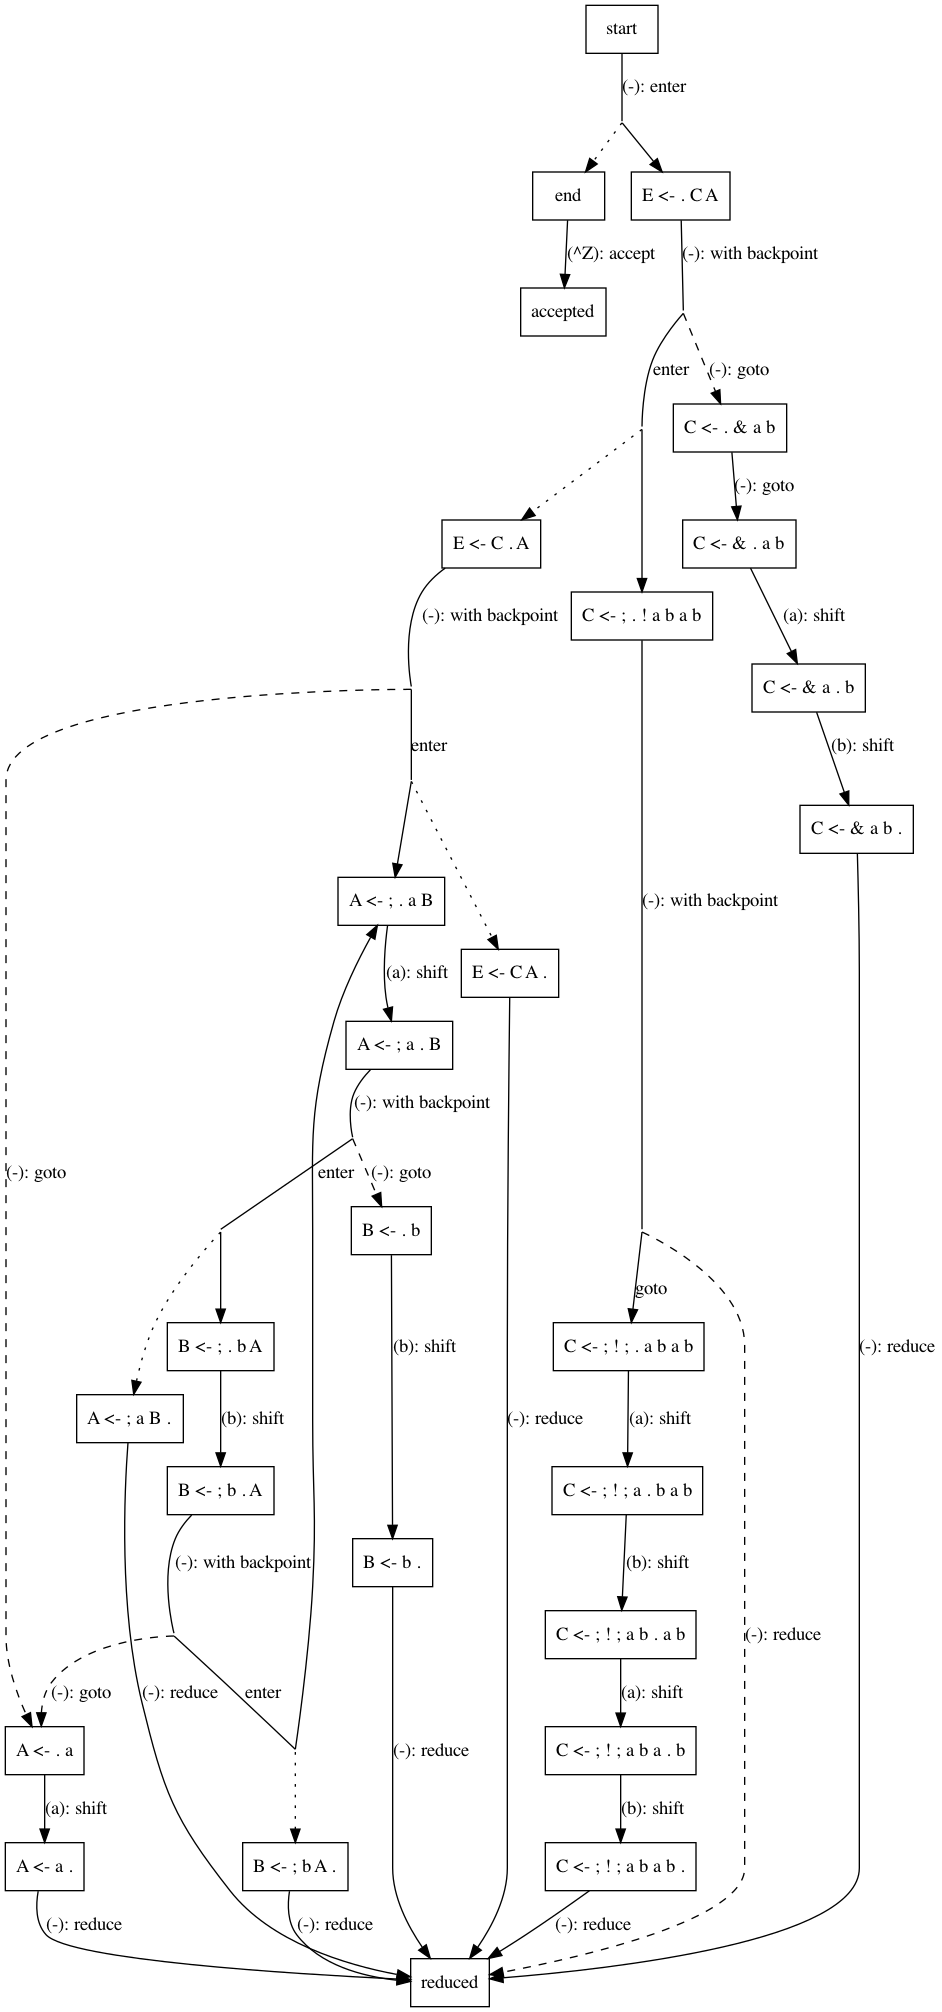
\includegraphics[height=0.9\textheight]{asset/implementation-note-of-peg-parser/sample-grammar.png}
  \caption{状態遷移図}
\end{figure}

\begin{figure}
  \centering
  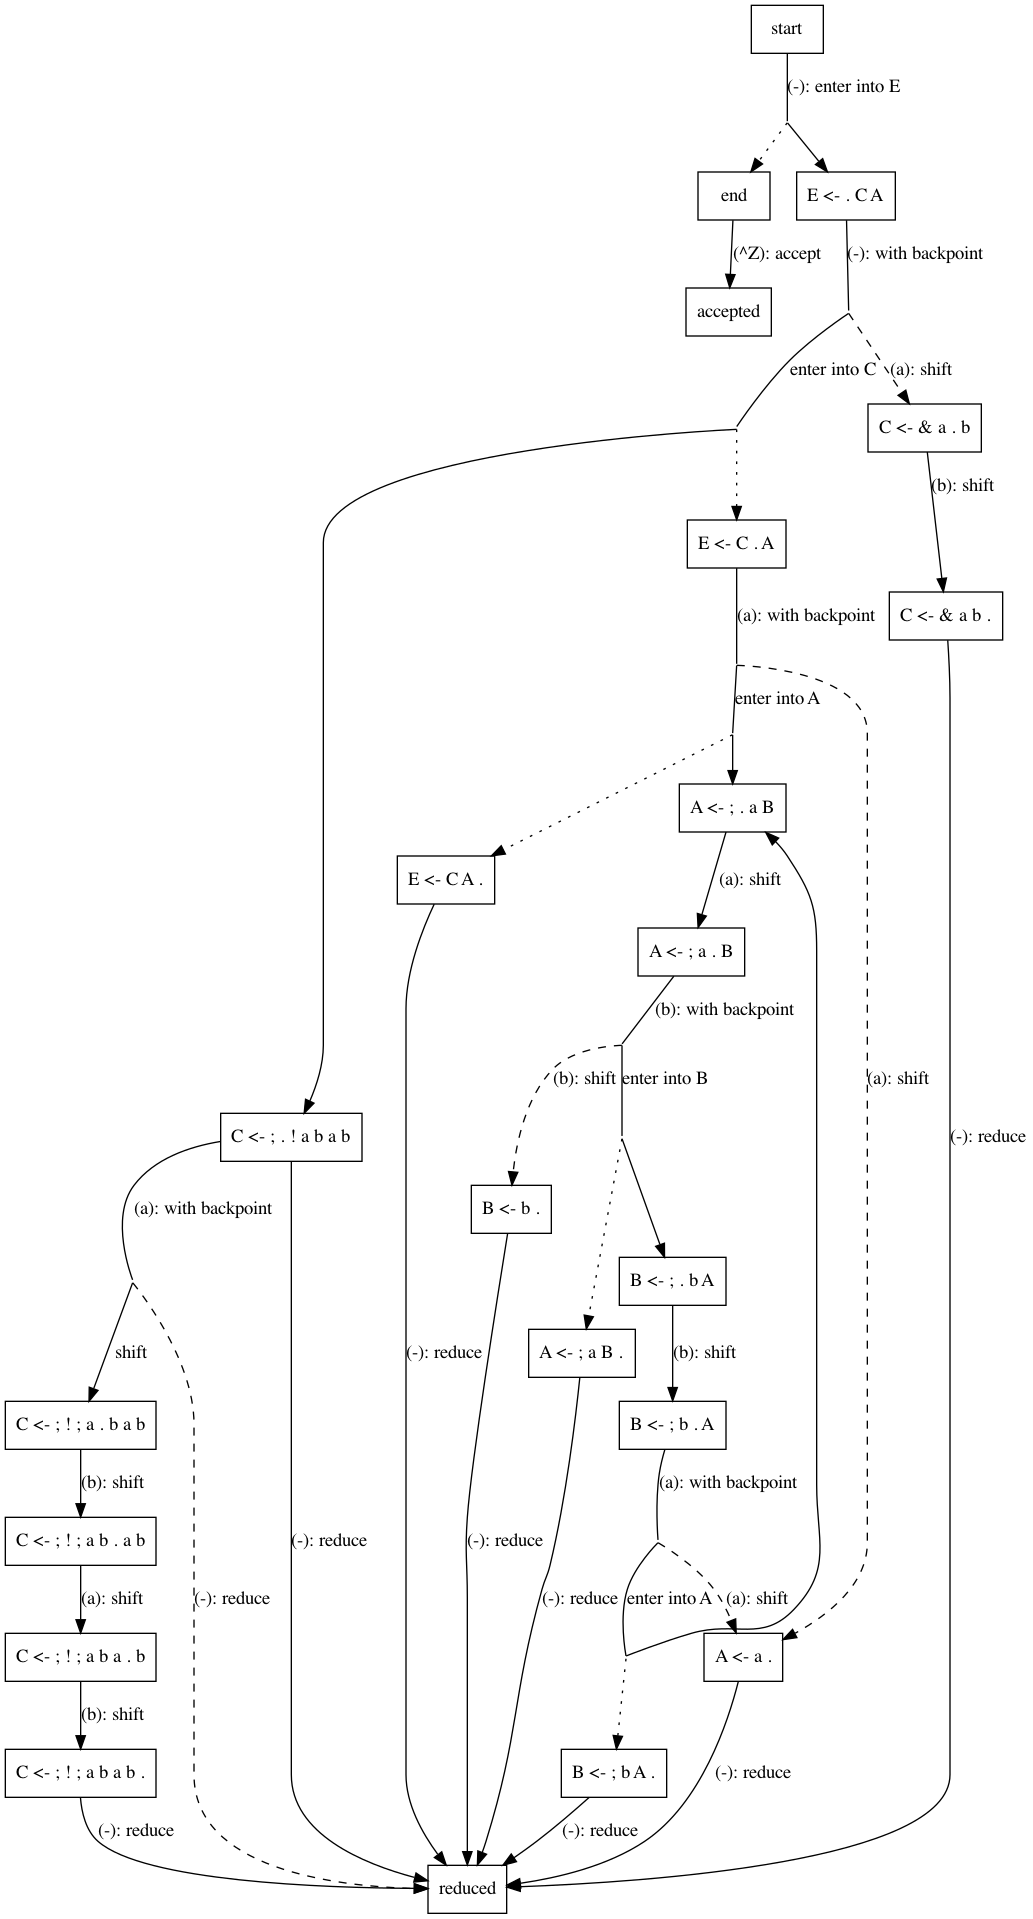
\includegraphics[height=0.9\textheight]{asset/implementation-note-of-peg-parser/sample-grammar-optimized.png}
  \caption{最適化された状態遷移図}
\end{figure}

\section{Quell Syntax and Identations}

\subsection{Syntax}

\section{Quell Modules}

\subsection{Syntax}

\begin{align*}
  \begin{array}{rcl}
  e
  & \Coloneq & \cdots \\
  & \mid & \symletrec \{B\} \symin e \\
  & \mid & P \\
  \tau
  & \Coloneq & \cdots \\
  & \mid & P \\
  P
  & \Coloneq & M \\
  M
  & \Coloneq & x \\
  & \mid & \{B\} \\
  & \mid & M.x \\
  & \mid & \symfun x: S\ldotp M \\
  & \mid & x\; x \\
  & \mid & x: S \\
  B
  & \Coloneq & x = e \\
  & \mid & \symtype t = T \\
  & \mid & \symmodule x = M \\
  & \mid & \symuse B \\
  & \mid & \epsilon \\
  & \mid & B; B \\
  T
  & \Coloneq & \lambda x\ldotp T \\
  & \mid & \tau \\
  S
  & \Coloneq & P \\
  & \mid & \{D\} \\
  & \mid & (x: S) \to S \\
  & \mid &
  \end{array}
\end{align*}


% foot contents
\bibliography{article/reference}

\appendix


\end{document}
